%\chapter{Spheroidal and Toroidal Oscillations}
\chapter{球型和环形振荡}
\label{chapter:sphericalearth}

自本章我们开始分析球对称、无自转地球模型的自由振荡。我们首先考虑具有各向同性应力-应变关系的地球模型,然后推广到横向各向同性地球模型。利用简正模式本征值问题的可分离性,可以将矢量和张量的控制方程转换为等价的径向标量方程系统,然后通过数值积分求解;这样基本上能够得到各向同性或横向各向同性地球模型的精确的本征频率~$\om$~和对应的本征函数~$\bs$。任何球对称、无自转地球模型都能够支持两种独立类型的自由振荡:对地球外部形状有改变的{\em 球型\/}振荡和没有改变的{\em 环型\/}振荡。我们将在第~11章和第12~章看到,简正模式的这两种类型的区别正是彼此独立传播的瑞利和勒夫面波以及~P-SV~和~SH~偏振的体波的驻波表现。}

\section{符号变更}
%\section{Change in Notation}

\begin{table}
\centering
\begin{tabular}{|l|c|c|} \hline
& & \\
变量名称或描述 & 旧符号 & 新符号 \\
& & \\ \hline
& & \\
初始密度 & $\rho^0$ & $\rho$ \\
\index{density}%
初始引力势函数 & $\phi^0$ & $\Phi$ \\
\index{gravitational potential}%
离心势函数 & $^{\dagger}$ & $\psi$ & $\psi$ \\
\index{centrifugal potential}%
& & \\
初始流体静力学压强 & $p^0$ & $p$ \\
\index{pressure!hydrostatic}%
\index{hydrostatic pressure}%
初始偏应力 & $\btau^0$ & $\btau$ \\
\index{stress!deviatoric}%
\index{deviatoric stress}%
负法向牵引力 & $\varpi^0$ & $\varpi$ \\
& & \\
等商不可压缩性$^{\dagger}$ & $\kappa$ & $\kappa$ \\
\index{incompressibility}%
\index{bulk modulus}%
\index{modulus!bulk}%
刚度$^{\dagger}$ & $\mu$ & $\mu$ \\
\index{rigidity}%
\index{shear modulus}%
\index{modulus!shear}%
压缩波速度$^{\dagger}$ & $\alpha$ & $\alpha$ \\
\index{compressional-wave speed}%
\index{P-wave speed}%
\index{speed!compressional-wave}%
剪切波速度$^{\dagger}$ & $\beta$ & $\beta$ \\
\index{shear-wave speed}%
\index{speed!shear-wave}%
\index{S-wave speed}%
&& \\
四阶弹性张量$^{\dagger}$ & $\bGamma$ & $\bGamma$ \\
\index{elastic tensor}%
\index{tensor!elastic}%
辅助弹性张量$^{\dagger}$ & $\bLambda$ & $\bLambda$ \\
各向异性弹性张量$^{\dagger}$ & $\bgamma$ & $\bgamma$ \\
& & \\
位移$^{\dagger}$ & $\bs$ & $\bs$ \\
\index{displacement}%
应变$^{\dagger}$ & $\beps$ & $\beps$ \\
\index{strain!deviatoric}%
\index{deviatoric strain}%
偏应变$^{\dagger}$ & $\bd$ & $\bd$ \\
& & \\
欧拉势函数微扰 & $\phi^{\rm E1}$ & $\phi$ \\
辅助引力矢量 & $\bxi^{\rm E1}$ & $\bxi$ \\
\index{gravity}%
& & \\
拉格朗日柯西应力增量 & $\bT^{\rm L1}$ & $\bT$ \\
\index{stress!Cauchy}%
\index{Cauchy stress}%
第一类$\rm Piola-Kirchhoff$应力增量 & $\bT^{\rm PK1}$ & $\widetilde{\bT}$ \\
\index{stress!first Piola-Kirchhoff}%
\index{Piola-Kirchhoff stress!first}%
辅助牵引力矢量 & $\bt^{\rm PK1}$ & $\tilde{\bt}$ \\
& & \\ \hline
\end{tabular}
\caption[newnotation]
{第~I~部分中所使用的符号与第~II、III~部分中使用的符号之间的对应关系。剑号所示无上角标变量的符号不变。我们之后将用~$-p\hspace{0.2 mm}{\bf I}+{\mbox{\boldmath $\bf \tau$}}$~表示总初始应力,用~$-{\mbox{\boldmath $\nabla$}}\cdot(\rho\hspace{0.2 mm}{\bf s})$~表示欧拉密度微扰,以免再为这些变量引入新的符号。}
\label{table:notation}
\end{table}

本书至此,我们一直用上角标~E~和~L~来小心地区分欧拉和拉格朗日动力学变量。
\index{Eulerian variable}%
\index{Lagrangian variable}%
此外,我们还一贯地用上角标~$0$~来标注平衡态地球模型中的参数,
\index{Earth model!equilibrium}%
\index{equilibrium Earth model}%
用上角标~$1$~来标注描述相对于平衡态构型(configurationxxx)的微扰的增量参数。既然已经建立了适用于一般地球模型的基本结果,摒弃这种虽然清楚但却凌乱的符号,而代之以一种不那么复杂的符号会更方便。表~\ref{table:notation}~概括列举了我们将在本书其余部分使用的这些新的“全无遮盖的”变量与第~Ⅰ~部分为清楚起见而使用的带上角标的变量之间的对应关系。表中所列的几个量,尤其是~$\btau$、$\varpi$、$\widetilde{\bT}$~和~$\tilde{\bt}$,在第Ⅱ部分关于球对称地球的讨论中并不会出现;但它们会在第Ⅲ部分对微弱非球对称地球的讨论中用到,因而被包含在此。需要说明的是,新的改进后的符号仍有不尽人意之处:我们用一个简单的~$\phi$~同时表示欧拉引力势函数微扰~$\phi^{\rm E1}$~和球极坐标系坐标~($r,\theta,\phi$)~中的经度。但是,我们相信这不会引起任何混肴,因为从上下文总能够明白它的含义。

%\section{SNREI Earth Model}
\section{SNREI~地球模型}
\index{SNREI Earth model|(}%
\index{Earth model!SNREI|(}%

SNREI~地球模型是一个球对称、无自转、完全弹性和各向同性的模型。最后一个形容词“各向同性”具有双重含义---初始应力是各向同性的,即偏应力为零,$\btau=\bzero$,以及四阶弹性张量~$\bGamma$~是各向同性的,其形式为:
\index{isotropic Earth model}%
\index{Earth model!isotropic}%
\eq \label{eq:8.firsteqn}
\Gamma_{ijkl}=(\kappa-\twothirds\mu)\delta_{ij}\delta_{kl}
+\mu(\delta_{ik}\delta_{jl}+\delta_{il}\delta_{jk}).
\en
一个一般的~SNREI~地球模型可通过给定其密度~$\rho$、等熵不可压缩性~$\kappa$~和刚度~$\mu$~作为距地心径向距离~$r$~的函数来完全描述。
\index{incompressibility}%
\index{bulk modulus}%
\index{modulus!bulk}%
\index{modulus!shear}%
\index{rigidity}%
\index{shear modulus}%
或者,我们也可以给定压缩波波速~$\alpha=[(\kappa+\fourthirds\mu)/\!\rho]^{1/2}$~和剪切波波速~$\beta=(\mu/\!\rho)^{1/2}$~的径向变化,来取代不可压缩性和刚度。图~\ref{fig:prem}~显示了各向同性的初步参考地球模型,以下简称~PREM~模型(Dziewonski \& Anderson \citeyear{dziewonski&anderson81}));
\index{Preliminary Reference Earth Model (PREM)}%
\index{shear-wave speed!PREM}%
\index{S-wave speed!PREM}%
\index{speed!shear-wave}%
\index{compressional-wave speed!PREM}%
\index{P-wave speed!PREM}%
\index{speed!compressional-wave}%
\index{density!PREM}%
其中,速度~$\alpha$~和~$\beta$~是由频率为~1 Hz~的~P~波或~S~波所“感受到的”。标准版的PREM~模型是横向各向同性且非弹性的;我们将在第~8.9~节和第~9.7~节中分别考虑这两种复杂性的影响。

\begin{figure}[!t]
\begin{center}
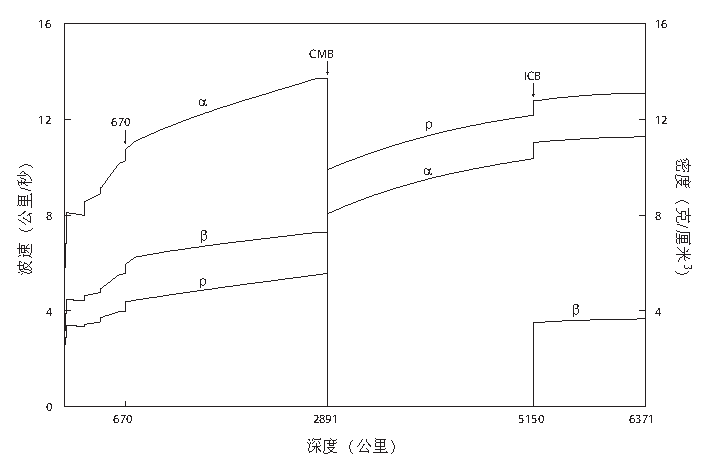
\includegraphics{../figures/chap08/fig01.eps}
\end{center}
\caption[PREM model]{\label{fig:prem}
“等效”各向同性初步参考地球模型(PREM)中的压缩波波速~$\alpha$、剪切波波速~$\beta$~和密度~$\rho$。图中标注了内核边界(ICB)和核幔边界(CMB)的位置。该模型顶部为一~3~公里厚的均匀海洋所覆盖。还有几个固—固界面,包括~24.4 km~深处的莫霍不连续面以及~220 km、400 km~和~670 km~深处的上地幔不连续面。
\index{boundary!interior}%
\index{interior boundary}%
最近的分析对全球性的~220 km~不连续面的存在提出了质疑,并改进了~400 km~和~670 km~不连续面的位置。}
\end{figure}
如同第Ⅰ部分,我们用~$\earth_{\rm S}$~表示地球所有固态区域的组合,用~$\earth_{\rm F}$~表示所有液态区域的组合,用~$\earth=\earth_{\rm S}\cup\earth_{\rm F}$~表示整个地球的体积。整个空间将仍用~$\allspace$~表示,因此~$\allspace -\earth$~表示地球外部的空间。对于如~PREM~一样的典型的~SNREI~地球模型,$\earth_{\rm S}$~的区域包含固态内核和地幔,而~$\earth_{\rm S}$~则包含液态的外核和海洋(我们在之后的讨论中将宽泛地用“地幔”一词表示地幔及上覆地壳)。
\index{boundary!solid-solid}%
\index{solid-solid boundary}%
\index{fluid-solid boundary}%
\index{boundary!fluid-solid}%
我们仍将继续用~$\Sigma_{\rm SS}$~表示所有内部的固-固不连续面的组合,用~$\Sigma_{\rm FS}$~表示所有固-液不连续面的组合,用~$\Sigma=\p\earth\cup\Sigma_{\rm SS}\cup\Sigma_{\rm FS}$~表示所有边界面包括外部自由表面的组合。球对称地球模型中界面~$\Sigma$~的向外的法向量~$\bnh$~是单位径向矢量~$\brh$;我们继续将~$\Sigma$~的外侧和内侧分别称为界面的~$+$~侧和~$-$~侧。

所有固-固不连续面的半径将统一用~$d_{\rm SS}$~表示,
\index{discontinuity!solid-solid}%
而所有固-液不连续面的半径将用~$d_{\rm FS}$~表示。
\index{discontinuity!fluid-solid}%
自由表面、核幔边界、内核边界和海底的半径分别用~$a$、$b$、$c$~和~$s$~表示。所有不连续面,包括外界面的半径的集合,将用~$d=a\cup d_{\rm SS}\cup d_{\rm FS}$~表示。在下文中为方便起见,我们定义~SNREI~地球模型的模型参数~$\rho$、$\kappa$、$\mu$、$\alpha$~和~$\beta$~在地球以外的~$r > a$~区域为零。我们将用任一仅依赖于半径的函数~$q$~上面的一点$\dot{q}$~来表示其导数~$dq /\hspace{-0.3 mm} dr$。
\index{derivative!radial}%
\index{radial derivative}%
\index{SNREI Earth model|)}%
\index{Earth model!SNREI|)}%

%\subsection{Gravity and hydrostatic pressure}
\subsection{重力和流体静力学压强}
\index{gravity|(}%
\index{pressure!hydrostatic|(}%
\index{hydrostatic pressure|(}%

SNREI~地球内部的重力场~$\bg=-\bdel\Phi$~是径向向下的:
\eq
\bg=-g\brh\quad\mbox{where}\quad g=\dot{\Phi}.
\label{eq:8.g}
\en
标量的重力加速度~$g=\|\bg\|$~满足一阶微分关系
\eq
\dg+2r^{-1}g=4\pi G\rho,
\label{eq:8.geq}
\en
其中$G$~为牛顿引力常数。可以很容易地将~(\ref{eq:8.geq})~式积分得到用密度分布~$\rho$~表示的~$g$~和对应的重力势函数~$\Phi$~的显式公式:
\eq
g(r)=\frac{4\pi G}{r^2}\int_0^r\rho'\,r^{\prime\hspace{0.3 mm}2}dr',
\qquad
\Phi(r)=-\frac{4\pi G}{r}\int_0^r\rho'\,r^{\prime\hspace{0.3 mm}2}dr',
\label{eq:8.gr}
\en
其中撇号表示在径向积分变量~$r'$~处取值。众所周知,一个球壳质量分布对其内部观察点的贡献为零,而一个球体对其外部观察点的引力与一个点质量等价。地球外部的重力加速度和势函数分别为~$g(r)=GM/r^2$~和~$\Phi(r)=-GM/r$,其中~$M=4\pi\int_0^a\rho\,r^2dr$~为地球的总质量。

SNREI地球模型的力学平衡由流体静力学平衡方程来保证:
\index{equilibrium!static}%
\index{static equilibrium}%
\eq
\dpp+\rho g=0,
\en
其中$p$~为初始流体静力学压强。对该方程也可以进行积分得到:
\eq
p(r)=\int_r^a\rho'g'\,dr',
\label{eq:8.pr}
\en
这里我们使用了自由表面边界条件~$p(a)=0$。PREM~模型中重力~$g$~和流体静力学压强~$p$~的径向变化如图~\ref{fig:premgrav&press}~所示。
%%%
\begin{figure}[!t]
\begin{center}
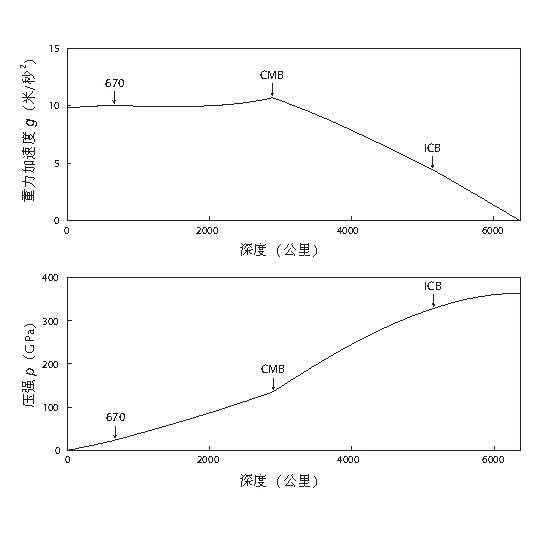
\includegraphics{../figures/chap08/fig02.eps}
\end{center}
\caption[PREM grav&stress]{\label{fig:premgrav&press}
初步参考地球模型中重力加速度~$g$~和流体静力学压强~$p$~随深度的变化。(上图)整个地幔中重力大致为常数~(9.8\hspace{0.2 mm}--10.1 m/${\rm s}^2$)。(下图)压强单调增加并在地心达到最大值~364 GPa。
\index{gravity!PREM}%
\index{pressure!PREM}%
}
\end{figure}

\index{gravity|)}%
\index{pressure!hydrostatic|)}%
\index{hydrostatic pressure|)}%

\renewcommand{\thesubsection}{$\!\!\!\raise1.3ex\hbox{$\star$}\!\!$
\arabic{chapter}.\arabic{section}.\arabic{subsection}}
%\subsection{Brunt-V\"{a}is\"{a}l\"{a} frequency}
\subsection{Brunt-V\"{a}is\"{a}l\"{a}~频率}
\index{Brunt-V\"{a}is\"{a}l\"{a} frequency|(}%
\index{frequency!Brunt-V\"{a}is\"{a}l\"{a}|(}%
\label{section:8.Brunt}
\renewcommand{\thesubsection}{\arabic{chapter}.\arabic{section}.\arabic{subsection}}

{\em Brunt-V\"{a}is\"{a}l\"{a}~频率\/}~$N(r)$一个值得关注的辅助参数,特别是在地球的液态区域~$\earth_{\rm FS}$内,其定义为:
\eq \label{8.Brunt}
N^2=-\frac{\drho g}{\rho}-\frac{\rho g^2}{\kappa}.
\en
这个量在物理上的重要性可通过考虑一小团流体的虚拟位移来理解(Eckart \citeyear{eckart60};Tolstoy \citeyear{tolstoy73})。为确定性起见,可以方便地将这团液体视为被松弛的薄膜所包覆,因而内部和外围环境压强始终相等,但又完全隔绝,因此在移动的流体内部其密度变化是绝热的。如果该团液体向上有一个无穷小移动~$\xi$,它将感受到一个压强变化~$\delta p=-\rho g\xi$,和一个绝热密度变化~$\delta\hspace{-0.2 mm}\rho_{\rm ad}
=\rho\kappa^{-1}\delta p=-\rho^2g\kappa^{-1}\xi$。
外围流体环境的密度变化却是不一样的~$\delta\hspace{-0.2 mm}\rho_{\rm am}=\dot{\rho}\hspace{0.2 mm}\xi$;因此,移动的这团流体受到单位体积上的浮力~$(\delta\hspace{-0.2 mm}\rho_{\rm am}
-\delta\hspace{-0.2 mm}\rho_{\rm ad})g=-\rho N^2\xi$的作用。令其与单位体积的惯性力相等,我们得到这一团绝热流体的运动方程:
\eq
\frac{d^2\xi}{dt^2}+N^2\xi=0.
\en
若~$N^2$~为正,这团流体将以角频率~$N$~在其初始平衡位置附近做正弦振荡;另一方面,若~$N^2$~为负,它将以指数形式远离其初始位置。流体中的密度分层在第一种情形中是重力稳定的,而在第二种情形中则是重力非稳定的;因此,$N$~有时被称为稳定性频率。
\index{stability frequency}%
\index{frequency!stability}%

对于密度梯度~$\drho$~偏离{\em Adams-Williamson\/}关系~$\drho=-\rho^2g/\kappa$~的程度有一个相关的度量是~\textcite{bullen63}~中的无量纲分层参数~$\eta_{\hspace{0.3 mm}\rm B}(r)$,
\index{Adams-Williamson relation}%
其定义为~$N^2=\rho g^2(\eta_{\hspace{0.3 mm}\rm B}-1)/\kappa$。
\index{Bullen stratification parameter}%
Bullen~的参数可以用不可压缩性参数对压强的导数重写为:
\eq
\eta_{\hspace{0.3 mm}\rm B}=\frac{d\kappa}{dp}+\frac{1}{g}\frac{d}{dr}
\!\left(\frac{\kappa}{\rho}\right).
\en
中性稳定的流体区域可以用两个等效的条件$N^2=0$和$\eta_{\hspace{0.3 mm}\rm B}=1$来描述。
\index{neutral stability}%
\index{stability!neutral}%

PREM~是通过用~$\rho$、$\alpha$~和~$\beta$~来拟合自由振荡和体波走时数据得到的,这种典型的~SNREI~地球模型的液态外核中有一些~$N^2>0$~和~$N^2<0$~交替变化的区域。但是,这些稳定与不稳定区域在物理上是不重要的,因为对~$N^2$~和~$\eta_{\hspace{0.3 mm}\rm B}$~都不能很好地约束;现有的地震学证据与液态外核处处呈中性分层的假设是一致的(Masters \citeyear{masters79})。严格来讲,PREM~中可压缩的、密度为常数的海水层也是不稳定的;这种情况就引起了一个现实问题---要分辨海水中实际的稳定分层结构将需要比任何全球地震学应用所要求的更精细的离散化。在第~8.8.2~节和~8.8.11~节中我们会看到,如果一个~SNREI~地球模型的~$\earth_{\rm F}$~区域中处处都有~$N^2=0$,那么计算所有可能存在的自由振荡的目录的工作会极大地简化。
\index{Brunt-V\"{a}is\"{a}l\"{a} frequency|)}%
\index{frequency!Brunt-V\"{a}is\"{a}l\"{a}|)}%

%\section{Equations of Motion}
\section{运动方程}
\index{equations of motion!SNREI Earth|(}%

SNREI~地球模型的自由振荡所满足的线性化运动方程及边界条件可以从第~3.11~节和第~4.3~节所讨论的无自转流体静力学地球模型的方程得到。用我们新的简化的符号,频率域动量方程~(\ref{4.nrhydromom})~可写为:
\eqa
\lefteqn{-\om^{2\!}\rho\hspace{0.2 mm}\bs-\bdel\cdot\bT
+(4\pi G\rho^2s_r)\brh+\rho\bdel_{\!}\phi} \nonumber \\
&&\mbox{}+\rho g[\bdel_{\!}s_r-(\bdel\cdot\bs+2r^{-1}s_r)\brh]
=\bzero,
\label{eq:8.smeq}
\ena
其中$s_r=\brh\cdot\bs$。我们利用了~(\ref{eq:8.geq})~式来消去~$\dg$~并将所有重力项整合起来。柯西应力增量~$\bT$~由各向同性本构关系给定:
\index{constitutive relation!isotropic}%
\eq
\bT=\kappa(\bdel\cdot\bs)\bI+2\mu\bd,
\label{eq:8.constitutive}
\en
其中~$\bd=\half[\bdel\bs+(\bdel\bs)^{\rm T}]
-\third(\bdel\cdot\bs)\bI$~为偏应变。利用运动学等式:
\eq
\brh\cdot\beps=\p_r\bs+\half\brh\times(\bdel\times\bs),
\label{eq:8.rde}
\en
我们可以仅用位移~$\bs$~和重力势函数增量~$\phi$~来将~(\ref{eq:8.smeq})~式写为
\eqa
\lefteqn{-\om^{2\!}\rho\hspace{0.2 mm}
\bs-(\kappa+\third\mu)\bdel(\bdel\cdot\bs)
-\mu\del^2\bs-(\dkappa-\twothirds\dmu)(\bdel\cdot\bs)\brh}
\label{eq:8.eqmot} \nonumber \\
&&\mbox{}-2\dmu[\p_r\bs
+\half\brh\times(\bdel\times\bs)]
+(4\pi G\rho^2s_r)\brh+\rho\bdel_{\!}\phi \nonumber \\
&&\mbox{}\qquad+\rho g[\bdel_{\!}s_r-(\bdel\cdot\bs+2r^{-1}s_r)\brh]
=\bzero.
\ena
矢量拉普拉斯算子的定义仍然是~$\del^2\bs=\bdel(\bdel\cdot\bs)
-\bdel\times(\bdel\times\bs)$。

运动学边界条件要求,除了固-液边界上允许切向滑动以外,位移要处处连续,
\index{boundary conditions!kinematic}%
即在~$\Sigma_{\rm SS}$~上有~$[\bs]_-^+=\bzero$和在$\Sigma_{\rm FS}$~上有~$[s_r]_-^+=0$。与~(\ref{4.hydrobc1})--(\ref{4.hydrobc3})~对应的动力学边界条件为
\eq
\brh\cdot\bT=\bzero\quad\mbox{在 $\p\earth$} 上,
\label{eq:8.df}
\en
\eq
[\brh\cdot\bT]_-^+=\bzero\quad\mbox{在 $\Sigma_{\rm SS}$ 上},
\label{eq:8.dss}
\en
\eq
[\brh\cdot\bT]_-^+=
\brh[\brh\cdot\bT\cdot\brh]^+_-=\bzero\quad\mbox{在 $\Sigma_{\rm FS}$ 上}.
\label{eq:8.dfs}
\en
(\ref{eq:8.rde})~式也可以用来得到任一球面上的牵引力增量的简单表达式,即
%%%
\eq
\brh\cdot\bT=(\kappa-\twothirds\mu)(\bdel\cdot\bs)\brh+2\mu(\p_r\bs)
+\mu\brh\times(\bdel\times\bs).
\label{eq:8.traction}
\en
在地球的液态区域,刚度~$\mu$~恒为零;因此,应力增量是流体静力学的,且相应的牵引力是纯径向的:$\bT=\kappa(\bdel\cdot\bs)\bI$~和~$\brh\cdot\bT=\kappa(\bdel\cdot\bs)\brh$。

重力势函数的欧拉微扰~$\phi$~由泊松方程的增量形式给定,在球对称地球中其形式为:
\index{Poisson's equation}%
\eq
\del^2\phi=-4\pi G(\rho\bdel\cdot\bs+\drho s_r).
\label{eq:8.poisson}
\en
势函数微扰必须处处连续,包括在所有边界~$\Sigma$~上,要有$[\phi]^+_-=0$。此外,我们还必须有:
\index{boundary conditions!gravitational}%
\eq
[\dphi+4\pi G\rho s_r]_-^+=0\quad\mbox{在 $\Sigma$上}.
\label{eq:8.ga}
\en
(\ref{eq:8.ga})~式的第二项源于与任一密度不连续面~$[\rho]^+_-$~的径向位移~$s_r$~相关的表观的面质量。若要得到~SNREI~地球模型的简正模式本征解~$\om$、$\bs$~和~$\phi$,我们必须在$\earth$中求得方程~(\ref{eq:8.eqmot})满足边界条件~(\ref{eq:8.df})--(\ref{eq:8.dfs})的解,并在$\allspace$中求得方程~(\ref{eq:8.poisson})
在~$\Sigma$~上满足边界条件~(\ref{eq:8.ga})的解。势函数增量~$\phi$~可由位移~$\bs$~以显式表示为
%%%
\eqa
\label{8.phiexpl}
\lefteqn{
\phi=G\int_{\subearth}\frac{(\rho'\bdel'\cdot\bs'+\drho's_r^{\prime})}
{\|\bx-\bx'\|}\,dV'+G\int_{\Sigma}\frac{[\rho']^+_-s_r^{\prime}}
{\|\bx-\bx'\|}\,d\/\Sigma'} \nonumber \\
&&\mbox{}=-G\int_{\subearth}\frac{\rho'\bs'\cdot(\bx-\bx')}
{\|\bx-\bx'\|^3}\,dV',
\ena
其中撇号表示在哑积分变量~$\bx'$~处取值,第二个等式来自高斯定理。
\index{equations of motion!SNREI Earth|)}%

%\section{Rayleigh's Principle}
\section{瑞利原理}
\index{Rayleigh's principle!SNREI Earth|(}%
\index{variational principle!SNREI Earth|(}%

SNREI~地球所满足的线性化弹性-重力运动方程和边界条件可由位移或位移-势函数形式的瑞利变分原理推导得到。前者的作用量是~(\ref{4.hydroact})~式的形式:
\index{action!SNREI Earth}%
\eq
\sI=\int_{\subearth}L(\bs,\bdel\bs)\,dV.
\label{eq:8.spaction}
\en
借助泊松方程~(\ref{eq:8.geq}),流体静力学拉格朗日量密度~(\ref{4.ZOOTME})~式可表示为
\index{Lagrangian density!SNREI Earth}%
\eqa
\lefteqn{L=\half[\om^{2\!}\rho\hspace{0.2 mm}
\bs\cdot\bs-\kappa(\bdel\cdot\bs)^2
-2\mu(\bd\!:\!\bd)-4\pi G\rho^2s_r^2}
\nonumber \\
&&\mbox{}-\rho\hspace{0.2 mm}\bs\cdot\bdel_{\!}\phi
-\rho g(\bs\cdot\bdel s_r-s_r\bdel\cdot\bs-2r^{-1}s_r^2)].
\label{eq:8.splagrangian}
\ena
(\ref{eq:8.splagrangian})~式中的势函数微扰~$\phi$~被视为位移~$\bs$~的已知泛函,由~(\ref{8.phiexpl})~式给定。对于任意可容许变化~$\bdelta\bs$,当且仅当~$\omega$~和~$\bs$~满足频率域动量方程~(\ref{eq:8.eqmot})~和动力学边界条件~(\ref{eq:8.df})--(\ref{eq:8.dfs})~时,变分~$\delta\sI$~为零。相应的修改后的作用量~(\ref{4.hydroact2})~为
\eq
\sI'=\int_{\subspace}
L'(\bs,\bdel\bs,\bdel_{\!}\phi)\,dV,
\label{eq:8.spaction2}
\en
其中
\eqa
\lefteqn{L'=\half[\om^{2\!}\rho\hspace{0.2 mm}
\bs\cdot\bs-\kappa(\bdel\cdot\bs)^2
-2\mu(\bd\!:\!\bd)-4\pi G\rho^2s_r^2}
\nonumber \\
&&\mbox{}-2\rho\hspace{0.2 mm}\bs\cdot\bdel_{\!}\phi
-\rho g(\bs\cdot\bdel s_r-s_r\bdel\cdot\bs-2r^{-1}s_r^2) \nonumber \\
&&\mbox{}\qquad-(4\pi G)^{-1}\bdel_{\!}\phi\cdot\bdel_{\!}\phi].
\label{eq:8.splagrang2}
\ena
对于任意且独立的可容许变化~$\bdelta\bs$~和~$\delta\phi$,当且仅当~$\phi$~和~$\bs$~由(\ref{eq:8.poisson})~和~(\ref{eq:8.ga})~相关联时,变分~$\delta\sI'$~为零。可容许位移变化~$\bdelta\bs$~在~$\Sigma_{\rm SS}$~上~$[\bdelta\bs]^+_-=\bzero$,且在~$\Sigma_{\rm FS}$~上满足~$[\delta s_r]^+_-=0$,
而可容许势函数变化~$\delta\phi$~在所有边界~$\Sigma$~上均满足~$[\delta\phi]^+_-=0$。对于所有本征解~$\om$、$\bs$、$\phi$,这两种作用量的稳定值为:
\eq
\label{8.actzero}
\sI=\sI'=0
\en
(\ref{8.actzero})这一结果可以通过用$\bs$与~(\ref{eq:8.smeq})式做点乘,以及用$(4\pi G)^{-1}\phi$与~(\ref{eq:8.poisson})式相乘,然后
分别在整个地球~$\earth$~和整个空间~$\allspace$~上积分来验证。
\index{Rayleigh's principle!SNREI Earth|)}%
\index{variational principle!SNREI Earth|)}%

\section{能量收支与稳定性}
%\section{Energy Budget and Stability}
\index{energy budget!SNREI Earth|(}%
\index{stability!SNREI Earth|(}%

在~SNREI~地球模型中,频率域能量密度~$E=\om\partial_\omega L-L$~由下式给定:
\eqa
\lefteqn{E=\half[\om^2\rho\hspace{0.2 mm}
\bs\cdot\bs+\kappa(\bdel\cdot\bs)^2
+2\mu(\bd\!:\!\bd)+4\pi G\rho^2s_r^2} \nonumber \\
&&\mbox{}+\rho\hspace{0.2 mm}\bs\cdot\bdel_{\!}\phi
+\rho g(\bs\cdot\bdel s_r-s_r\bdel\cdot\bs-2r^{-1}s_r^2)].
\ena
\index{energy!total}%
\index{total energy}%
\index{kinetic energy}%
\index{potential energy}%
\index{energy!kinetic}%
\index{energy!potential}%
振荡的一个简正模式的总积分能量是其动能与弹性-重力势能之和:
\eq
\sE=\half(\om^2\sT+\sV),
\en
其中
\eq
\sT=\int_{\subearth}\rho\hspace{0.2 mm}
\bs\cdot\bs\,dV. \label{eq:8.kineticenergy}
\en
(\ref{8.actzero})~式可以被解释为一个能量{\em 均分\/}关系,$\om^2\sT=\sV$,
\index{energy equipartition}%
\index{equipartition relation}%
因而一个振荡的总能量简单的就是其动能的两倍:$\sE=\om^2\sT$。势能可以进一步分解为不同的{\em 压缩弹性势能\/}、{\em 剪切弹性势能\/}和{\em 重力势能\/}:
\index{energy!compressional}%
\index{bulk energy}%
\index{shear energy}%
\index{compressional energy}%
\index{energy!bulk}%
\index{energy!shear}%
\index{energy!gravitational}%
\index{gravitational energy}%
\index{compressional energy}%
\eq \label{8.potener}
\sV=\sV_{\kappa}+\sV_{\mu}+\sV_{\rm g},
\en
其中
\eq
\sV_{\kappa}=\int_{\subearth}\kappa(\bdel\cdot\bs)^2\,dV,
\label{eq:8.bulkenergy}
\en
\eq
\sV_{\mu}=\int_{\subearth}2\mu(\bd\!:\!\bd)\,dV,
\label{eq:8.shearenergy}
\en
\vspace{-2.0 mm}
\eqa \label{eq:8.gravenergy}
\lefteqn{\sV_{\rm g}=\int_{\subearth}\rho\hspace{0.2 mm}[4\pi G\rho s_r^2
+\bs\cdot\bdel\phi} \nonumber \\
&&\mbox{}\qquad\qquad
+g(\bs\cdot\bdel s_r-s_r\bdel\cdot\bs-2r^{-1}s_r^2)]\,dV.
\ena
在第~\ref{sec:8.spherfigs}~节中我们将看到,一个球型简正模式如何将其势能在~$\sV_{\kappa}$、$\sV_{\mu}$~和~$\sV_{\rm g}$~中分配是它的主要识别标志之一。

在第~\ref{4.sec.stable}~节我们讨论过,对于在~$r=d_{\rm FS}$~处满足~$[s_r]^+_-=0$~的分段平滑位移~$\bs$,只有当势能泛函~(\ref{8.potener})~为非负,即~$\sV_{\kappa}+\sV_{\mu}+\sV_{\rm g}\geq 0$时,SNREI~地球模型才是动态稳定的。
\index{dynamical stability!SNREI Earth}%
\index{stability!dynamical!SNREI Earth}%
压缩能~$\sV_{\kappa}$~和剪切能~$\sV_{\mu}$~在本质上都是非负的;相反,重力能~$\sV_{\rm g}$~的可正可负,因而重力可能起到稳定或失稳的作用,取决于振荡的形状。应用高斯定理并重整各项,我们可以用~(\ref{8.Brunt})~式中定义的~Brunt-V\"{a}is\"{a}l\"{a}~频率~$N$~将势能写为
\eqa
\label{8.VBrunt}
\lefteqn{\sV=\int_{\subearth}[\kappa
(\bdel\cdot\bs-\kappa^{-1}\rho g s_r)^2+
2\mu(\bd\!:\!\bd)+\rho N^2 s_r^2]\,dV} \nonumber \\
&&\mbox{}-\frac{1}{4\pi G}\int_{\subspace}
\bdel_{\!}\phi\cdot\bdel_{\!}\phi\,dV
-\int_{\Sigma}[\rho]^+_-g s_r^2\,d\/\Sigma.
\ena
(\ref{8.VBrunt})~式显示,对于所有短波长形变(重力势函数微扰~$\phi$~可以忽略不计),只要在$0\leq r\leq a$范围内~$N^2\geq 0$,且在~$r=d$~时~$[\rho]^+_-\leq 0$,SNREI地球模型就是{\em 局部\/}稳定的。
\index{deformation!short-wavelength}%
\index{short-wavelength deformation}%
\index{stability!local}%
\index{local stability}%
事实上,可以证明这两个条件能够使一个模型对{\em 一切非径向的\/}微扰都是{\em 全局\/}稳定的。
\index{stability!global}%
\index{global stability}%
这一全局稳定性结果的证明过于冗长,这里不再赘述;它通过对含有~$\bdel\phi\cdot\bdel\phi$~一项做“巧妙的”变换,再与一些“标准的”不等式一起,来证明对于满足约束~$\int_{\Omega}\phi\,d\/\Omega=0$~的所有变形均有~$\sV\hspace{0.5mm}\geq\hspace{0.5mm}0$~(Aly \& P\'{e}rez \citeyear{aly&perez92})。\vspace{-0.4 mm}
对于一个液态球($\mu=0$),其物理上合理的条件~$N^2\geq 0$~和~$[\rho]^+_-\leq 0$~是非径向稳定性的充要条件;该结果在天体物理学中被称为~{\em Antonov-Lebovitz定理\/}~(Binney \& Tremaine \citeyear{binney&tremaine87})。
\index{Antonov-Lebovitz theorem}%

通过将引力常数~$G$、重力加速度~$g$~和势函数微扰~$\phi$~都设为零,本节和前两节中的所有关系式~(\ref{eq:8.smeq})--(\ref{8.VBrunt})~都可以做{\em 无重力极限\/}的简化。
\index{non-gravitating limit}%
所得到的结果就是经典的各向同性弹性体所满足的动量方程、边界条件和相应的拉格朗日量与能量密度。这样的弹性体本质上是稳定的,因为其势能全部是弹性的:$\sV=\sV_{\kappa}+\sV_{\mu}\geq 0$。
\index{energy budget!SNREI Earth|)}%
\index{stability!SNREI Earth|)}%

%\section{Radial Scalar Equations}
\section{径向标量方程}
\index{radial equations|(}%
\label{sec:8.radscaleqns}

为了计算~SNREI~地球模型的本征频率和本征函数,我们需要将线性化的运动方程和相应的边界条件转化为一组等价的耦合标量方程。我们将用三种不同的方法来完成这项重要的工作。第一种是用直接的暴力的做法,仅采用附录~B中所回顾的经典的标量场和矢量场的球谐函数表述。第二种方法在推导上不那么繁琐,但需要更多的理论基础;它是基于附录~C中所讨论的任意张量场的广义球谐函数表述。最后的第三种方法是利用瑞利原理;它的第一步是要得到作用量~$\sI$~和~$\sI'$~的等价的标量表达式。在继续下面的讨论之前,对普通或球谐函数的几何和代数性质不熟悉的读者,可能要先阅读一下附录~B~和附录~C。

%\subsection{Approach 1: Vector spherical harmonics}
\subsection{方法1:矢量球谐函数}
\label{section:8.ap1}

我们采用原点在~SNREI~地球球心的球极坐标系坐标~$r$, $\theta$, $\phi$,来寻求方程组~(\ref{eq:8.eqmot})--(\ref{eq:8.dfs})~和~(\ref{eq:8.poisson})--(\ref{eq:8.ga})~具有如下分离变量形式的本征解:
\eq
\bs=U\bP_{lm}+V\bB_{lm}+W\bC_{lm},\qquad\phi=P\ylm,
\label{eq:8.repr}
\en
其中的{\em 径向本征函数\/}~$U(r)$, $V(r)$, $W(r)$~和~$P(r)$~仅为半径的函数。
\index{eigenfunction!radial}%
\index{radial eigenfunction}%
次数为$0\leq l\leq\infty$,阶数为~$-l\leq m\leq l$~的实数的标量和矢量球谐函数~$\ylm$~和~$\bP_{lm}$, $\bB_{lm}$, $\bC_{lm}$~的定义为
\eqa \label{8.realYdef} \lefteqn{
\ylm(\theta,\phi)=\left(\frac{2l+1}{4\pi}\right)^{\!1/2}\frac{1}{2^ll!}
\left[\frac{(l-|m|)!}{(l+|m|)!}\right]^{1/2}} \nonumber \\
&&\qquad\mbox{}\times (\sin\theta)^{|m|}
\left(\frac{1}{\sin\theta}\frac{d}{d\theta}\right)^{l+|m|}
(\sin\theta)^{2l} \nonumber \\
&&\qquad\mbox{}\times\left\{\begin{array}{ll}
\sqrt{2}\cos m\phi
& \mbox{if $-l\leq m<0$} \\
\vspace{-5.5 mm} & \vspace{2.0 mm} \\
1 & \mbox{if $m=0$} \\
\vspace{-5.5 mm} & \vspace{2.0 mm} \\
\sqrt{2}\sin m\phi
& \mbox{if $0<m\leq l$}
\end{array}\right.
\ena
和
\begin{displaymath}
\bP_{lm}(\theta,\phi)=\brh\,\ylm(\theta,\phi),\qquad
\bB_{lm}(\theta,\phi)=\sqLinv \bdel_1\ylm(\theta,\phi),
\end{displaymath}
\eq \label{8.PBClm}
\qquad\qquad\bC_{lm}(\theta,\phi)=
-\sqLinv(\brh\times\bdel_1)\ylm(\theta,\phi).
\en
~(\ref{8.PBClm})~式中的无量纲切向矢量算子~$\bdel_1=\bthetah\p_{\theta}+\bphih(\sin\theta)^{-1}\p_{\phi}$和$\brh\times\bdel_1=-\bthetah(\sin\theta)^{-1}\p_{\phi}
+\bphih\p_{\theta}$~是单位球~$\Omega$~上的表面梯度和旋度,并且
\eq
\label{8.kdef}
\sqL=\sqrt{l(l+1)}.
\en
我们将在第~11~章和~12~章中看到,$k$~这个量是在~$l\rightarrow\infty$~极限下与振荡的简正模式相对应的体波或面波行波的渐近角{\em 波数\/}。
\index{wavenumber}%
但是,对于目前更普遍的情形,(\ref{8.kdef})~式只是一个适用于所有球谐函数角次数~$0\leq l\leq\infty$~的定义。

在附录~B.12~中证明了~$\bdel\cdot\bs$、$\bdel\times\bs$、$\bdel(\bdel\cdot\bs)$、$\bdel\times\bdel\times\bs$~和~$\nabla^2\bs=
\bdel(\bdel\cdot\bs)-\bdel\times(\bdel\times\bs)$~这些量可以用径向本征函数~$U$、$V$~和~$W$表示为:
%%%
\eq
\bdel\cdot\bs=[\dU+r^{-1}(2U-\sqL V)]\ylm,
\label{eq:8.diver}
\en
\eqa
\lefteqn{\bdel\times\bs=(\sqL r^{-1}W)\bP_{lm}
+(\dW+r^{-1}W)\bB_{lm}} \nonumber \\
&&\mbox{}-[\dV+r^{-1}(V-\sqL U)]\bC_{lm},
\label{eq:8.curl}
\ena
\eqa
\lefteqn{\bdel(\bdel\cdot\bs)=[\ddU+r^{-1}(2\dU-\sqL\dV)
-r^{-2}(2U-\sqL V)]\bP_{lm}} \nonumber \\
&&\mbox{}+\sqL r^{-1}[\dU+r^{-1}(2U-\sqL V)]\bB_{lm},
\ena
\eqa
\lefteqn{\bdel\times\bdel\times\bs=
-\sqL r^{-1}[\dV+r^{-1}(V-\sqL U)]\bP_{lm}} \nonumber \\
&&\mbox{}-(\ddV+2r^{-1}\dV-\sqL r^{-1}\dU)\bB_{lm} \nonumber \\
&&\mbox{}\qquad-(\ddW+2r^{-1}\dW-\sqL^2r^{-2}W)\bC_{lm},
\label{8.curl2}
\ena
\eqa
\lefteqn{\del^2\bs=[\ddU+2r^{-1}\dU-2r^{-2}U
+\sqL r^{-2}(2V-\sqL U)]\bP_{lm}} \nonumber \\
&&\mbox{}+[\ddV+2r^{-1}\dV+\sqL r^{-2}(2U-\sqL V)]\bB_{lm} \nonumber \\
&&\mbox{}\qquad+(\ddW+2r^{-1}\dW-\sqL^2r^{-2}W)\bC_{lm}.
\label{eq:8.Lapla}
\ena
将展开式~(\ref{eq:8.repr})~和~(\ref{eq:8.diver})--(\ref{eq:8.Lapla})~代入线性化运动方程~(\ref{eq:8.eqmot})~中,并将依赖于球谐函数~$\bP_{lm}$、$\bB_{lm}$、$\bC_{lm}$~的项整理在一起,我们得到三个二阶常微分方程:
\eqa
\lefteqn{r^{-2}\frac{d}{dr}[r^2(\kappa+\fourthirds\mu)\dU
+(\kappa-\twothirds\mu) r(2U-\sqL V)]}
\label{eq:8.U} \nonumber \\
&&\mbox{}+r^{-1}[(\kappa+\fourthirds\mu)\dU
+(\kappa-\twothirds\mu) r^{-1}(2U-\sqL V)] \nonumber \\
&&\mbox{}\qquad
-3\kappa r^{-1}(\dU+2r^{-1}U-\sqL r^{-1}V) \\
&&\mbox{}\qquad\qquad-\sqL\mu r^{-1}(\dV-r^{-1}V+\sqL r^{-1}U)+\om^{2\!}\rho U
\nonumber \\
&&\mbox{}\qquad\qquad\qquad-\rho[\dP
+(4\pi G\rho-4gr^{-1})U+\sqL gr^{-1}V]=0, \nonumber
\ena
\eqa
\lefteqn{r^{-2}\frac{d}{dr}[\mu r^2(\dV-r^{-1}V+\sqL r^{-1}U)]
+\mu r^{-1}(\dV-r^{-1}V+\sqL r^{-1}U)}
\label{eq:8.V} \nonumber \\
&&\mbox{}+\sqL(\kappa-\twothirds\mu)r^{-1}\dU
+\sqL(\kappa+\third\mu)r^{-2}(2U-\sqL V) \\
&&\mbox{}\qquad+[\om^{2\!}\rho-(\sqL^2-2)\mu r^{-2}]V
-\sqL\rho r^{-1}(P+gU)=0, \nonumber
\ena
\eqa
\lefteqn{r^{-2}\frac{d}{dr}[\mu r^2(\dW-r^{-1}W)]
+\mu r^{-1}(\dW-r^{-1}W)}
\label{eq:8.W} \nonumber \\
&&\mbox{}+[\om^{2\!}\rho-(\sqL^2-2)\mu r^{-2}]W=0.
\ena
用径向本征函数,固-固边界~$\Sigma_{\rm SS}$~和固-液边界~$\Sigma_{\rm FS}$~上的运动学连续性条件可以分别表示为:在~$\Sigma_{\rm FS}$~上,$[U]_-^+=[V]_-^+=[W]_-^+=0$;在~$r=d_{\rm FS}$~时,$[U]_-^+=0$。

作用在任一球面上的牵引力~(\ref{eq:8.traction})~可以用位移标量函数~$U$、$V$~和~$W$~表示为
\eq
\label{8.rdotT}
\brh\cdot\bT=R\bP_{lm}+S\bB_{lm}+T\bC_{lm},
\en
其中
\eq
\label{8.tract1}
R=(\kappa+\fourthirds\mu)\dU
+(\kappa-\twothirds\mu)r^{-1}(2U-\sqL V),
\en
\eq
S=\mu(\dV-r^{-1}V+\sqL r^{-1}U),
\en
\eq
\label{8.tract2}
T=\mu(\dW-r^{-1}W).
\en
表示在各种边界上牵引力连续性的动力学边界条件~(\ref{eq:8.df})--(\ref{eq:8.dfs})~意味着
\eq \label{8.bcneed}
R=S=T=0\quad\mbox{当 $r=a$时,}
\en
\eq
[R]^+_-=[S]^+_-=[T]^+_-=0\quad\mbox{当 $r=d_{\rm SS}$时,}
\en
\eq
[R]^+_-=S=T=0\quad\mbox{当 $r=d_{\rm FS}$时.}
\label{eq:8.dfsT}
\en
在液态区域~$\earth_{\rm F}$~内,由于刚度为零~$\mu=0$,故剪切牵引力~$S$~和~$T$~处处为零。
因此,$\dV-r^{-1}V+\sqL r^{-1}U$~和~$\dW-r^{-1}W$~这两个量在~$\dW-r^{-1}W$~的固态一侧也必须为零。

泊松方程~(\ref{eq:8.poisson})~等价于二阶常微分方程
\index{Poisson's equation}%
\eqa \label{eq:8.P} \lefteqn{
\ddP+2r^{-1}\dP-\sqL^2r^{-2}P} \nonumber \\
&&\mbox{}=-4\pi G\drho\hspace{0.2 mm}U
-4\pi G\rho[\dU+r^{-1}(2U-\sqL V)].
\ena
相应的重力边界条件为~$[P]^+_-=0$,以及
\eq
[\dP+4\pi G\rho\hspace{0.2 mm}U]_-^+=0
\quad\mbox{当 $r=d$时.}
\label{eq:8.ap}
\en
通过代入,很容易证明边值问题~(\ref{eq:8.P})--(\ref{eq:8.ap})~的解为
\eqa
\label{8.Pexplicit}
\lefteqn{P(r)=-\frac{4\pi G}{2l+1}\left\{r^{-l-1}\int_0^r
\rho'[lU'+\sqL V']r^{\prime\,l+1}\,dr'\right.} \nonumber \\
&&\mbox{}+\left.r^l\int_r^a\rho'[-(l+1)U'+\sqL V']
r^{\prime\,-l}\,dr'\right\} \nonumber \\
&&\mbox{}\qquad\qquad\qquad\qquad\mbox{在 $0\leq r\leq a$时},
\ena
\eqa
\label{8.Pexplicit2}
\lefteqn{P(r)=-\frac{4\pi G}{2l+1}\left\{r^{-l-1}\int_0^a
\rho'[lU'+\sqL V']r^{\prime\,l+1}\,dr'\right\}} \nonumber \\
&&\mbox{}\qquad\qquad\qquad\qquad\mbox{在 $a\leq r\leq\infty$时}.
\ena
(\ref{8.Pexplicit})和~(\ref{8.Pexplicit2})~两式以显式将欧拉势函数微扰~$P$用~$U$~和~$V$~表示,是与~(\ref{8.phiexpl})~式对应的标量形式。(\ref{eq:8.U})--(\ref{8.Pexplicit2})~这些结果是\textcite{pekeris&jarosch58}用上述暴力方式首次得到的。在这一经典工作中,由于作者对~(\ref{8.PBClm})~中的~$\bB_{lm}$~和~$\bC_{lm}$~所做的定义不同,因此他们的切向标量函数~$V$~和~$W$~要比我们所定义的小了一个因子~$\sqL$。另外一些开拓性的自由振荡研究,包括~Backus \& Gilbert (\citeyear{backus&gilbert67})~和~Woodhouse (\citeyear{woodhouse80}),也使用了这种不同的矢量球谐函数定义。

%\subsection{Decoupling and degeneracy}
\subsection{解耦与简并}
\index{degeneracy|(}%
\index{eigenfrequency degeneracy|(}%

对公式~(\ref{eq:8.U})--(\ref{8.Pexplicit2})加以检视,可以使我们得出两个重要的发现。首先,确定径向本征函数~$U$、$V$~和~$P$~与确定~$W$~的是完全解耦的。因此,SNREI~地球模型具有两种截然不同的简正模式类型:位移形式为~$U\bP_{lm}+V\bB_{lm}$~的{\em 球型\/}模式和位移形式为~$W\bC_{lm}$~的{\em 环型\/}模式。
\index{spheroidal mode}%
\index{mode!spheroidal}%
\index{toroidal mode}%
\index{mode!toroidal}%
球型振荡会改变地球的外部形状和内部密度;因此,它们是伴随有重力势函数微扰~$P\ylm$的。相反,环型振荡具有纯切向位移和零散度;因此,它们不会影响地球的形状和径向密度分布$\rho$。无论是否考虑地球的重力,其环型模式的径向方程和边界条件都是一样的。第二,我们注意到所有的径向本征函数~$U$、$V$、$P$~和~$W$~所遵循的标量方程都不依赖于方位角阶数~$m$。因此,每一个球型或环型本征频率~$\om$~都是{\em 简并的\/},
\index{degeneracy}%
具有一个由实的表面球谐函数~$\sY_{l\,-l},\ldots,
\sY_{l0},\ldots,\sY_{ll}$~所展布的~$(2l+1)$~维本征空间。这个~$(2l+1)$~重简并是模型的球对称性质所预期的数学结果。

每当需要区分~SNREI~地球的本征频率与本征函数时,我们会使用诸如~${}_n\om_l^{\rm S}$、${}_n\om_l^{\rm T}$~
和~${}_nU_l$、${}_nV_l$、${}_nW_l$~这样的角标符号。
预期到对于球谐函数次数~$l$~的每个给定值,都会有无穷多个球型和环型模式,它们的本振频率~${}_n\om_l^{\rm S}$~和~${}_n\om_l^{\rm T}$~在~$n\rightarrow\infty$~时也趋于无穷这一现象,我们引入了{\em 径向阶数\/}~这一前角标$n=0,1,2,\ldots$。
\index{overtone number}%
与给定本征频率~${}_n\om_l^{\rm S}$~或~${}_n\om_l^{\rm T}$~所对应的~$2l+1$~个振荡被称为{\em 多态模式\/},
\index{multiplet}%
分别用~${}_n{\rm S}_l$~和${}_n{\rm T}_l$~来表示球型模式和地幔的环型模式。
多态模式~${}_n{\rm S}_l$~中的每个球型本征函数~${}_nU_l\bP_{lm}+{}_nV_l\bB_{lm}$~和多态模式~${}_nW_l\bC_{lm}$~中的每个环型本征函数~${}_nW_l\bC_{lm}$~被称为{\em 单态模式\/}。
\index{singlet}%
对极轴($\theta=0$)和零子午线($\phi=0$)的每一种不同的选择会导致不同的球谐函数~$\sY_{l\,-l},\ldots,
\sY_{l0},\ldots,\sY_{ll}$,于是每个多态模式会有~$2l+1$~个不同的单态模式构成的基函数展布于其中。地球模型相对于球对称的任何偏离都会解除本征频率的简并,并导致多态模式~${}_n{\rm S}_l$~和~${}_n{\rm T}_l$~的分裂与耦合,相关内容将在第~13--14~章中讨论。作为一般的规则,只要能够保证意义明晰,我们将在本征频率~$\omega$~和本征函数~$U,V,W$~的符号上使用最少的辨识性的上角标~${\rm S},{\rm T}$~和下角标~$n,l,m$。通常情况下,我们会像在~(\ref{eq:8.repr})~式中那样,省略多态模式的标识,以避免符号上过于杂乱。
\index{degeneracy|)}%
\index{eigenfrequency degeneracy|)}%

\renewcommand{\thesubsection}{$\!\!\!\raise1.3ex\hbox{$\star$}\!\!$
\arabic{chapter}.\arabic{section}.\arabic{subsection}}
%\subsection{Approach 2: Generalized spherical harmonics}
\subsection{方法2:广义球谐函数}
\label{section:8.ap2}
\renewcommand{\thesubsection}{\arabic{chapter}.\arabic{section}.\arabic{subsection}}

在广义球谐函数表述中,矢量和张量不是用习惯上的实数基~$\brh$、$\bthetah$、$\bphih$,而是由以下所谓的{\em 正则基\/}来表示的:
\index{canonical basis}%
\index{basis!canonical}%
\eq \label{8.canbasis}
\beh_-=\textstyle{\frac{1}{\sqrt{2}}}(\bthetah-i\bphih),\qquad
\beh_0=\brh,\qquad
\beh_+=-\textstyle{\frac{1}{\sqrt{2}}}(\bthetah+i\bphih),
\en
在下文中,希腊字母角标~$\alpha,\beta,\gamma,\ldots$~用来表示相对于~(\ref{8.canbasis})~中的矢量的分量,取值范围为~$\{-,0,+\}$。此时,位移和重力势函数微扰~(\ref{eq:8.repr})~可写为如下形式
\eq \label{8.srepr}
\bs=s^-Y_{lm}^{-1}\beh_-
+s^0Y_{lm}^0\beh_0+s^+Y_{lm}^1\beh_+,\qquad
\phi=PY_{lm}^0,
\en
其中的正则分量~$s^{\alpha}$~仅依赖于半径。应变张量~$\beps$~可用类似的方式表示,即
\eqa
\lefteqn{\beps=\eps^{--}Y_{lm}^{-2}\beh_-\beh_-
+\eps^{0-}Y_{lm}^{-1}(\beh_0\beh_-+\beh_-\beh_0)} \nonumber \\
&&\mbox{}+(\eps^{00}+2\eps^{-+})Y_{lm}^0\beh_0\beh_0
+\eps^{0+}Y_{lm}^{1}(\beh_0\beh_++\beh_+\beh_0) \nonumber \\
&&\mbox{}\qquad+\eps^{++}Y_{lm}^{2}\beh_+\beh_+.
\label{eq:8.strain}
\ena
对称性~$\beps=\beps^{\rm T}$~保证了~$\eps^{\alpha\beta}=\eps^{\beta\alpha}$。$\bs$、$\phi$~和~$\beps$~的角度依赖性包含在次数为~$0\leq l\leq\infty$,阶数为~$-l\leq m\leq l$,和上角标为~$-l\leq N\leq l$~的复数{\em 广义球谐函数\/}~$Y_{lm}^N$~中,
\index{generalized spherical harmonics}%
\index{spherical harmonics!generalized}%
其定义为
\eqa
\lefteqn{Y_{lm}^N(\theta,\phi)=\left(\frac{2l+1}{4\pi}\right)^{1/2}
\left[\frac{1}{(l+N)!(l-N)!}\right]^{1/2}
\left[\frac{(l-m)!}{(l+m)!}\right]^{1/2}} \nonumber \\
&&\mbox{}\times2^{l+m}(\sin\half\theta)^{m-N}
(\cos\half\theta)^{m+N} \nonumber \\
&&\mbox{}\times\left(\frac{1}{\sin\theta}
\frac{d}{d\theta}\right)^{l+m}
\left[(\sin\half\theta)^{2l+2N}(\cos\half\theta)^{2l-2N}\right]
\nonumber \\
&&\mbox{}\times\exp(im\phi).
\ena
要注意,仅需要~$Y_{lm}^0$、$Y_{lm}^{\pm 1}$~和~$Y_{lm}^{\pm 2}$~来表示标量、向量和二阶张量场~(\ref{8.srepr})--(\ref{eq:8.strain})。

应变~$\eps^{\alpha\beta}$~的六个独立正则分量与位移的三个分量~$s^{\alpha}$~之间的关系为
\eq \label{8.strain1}
\eps^{00}=\ds^0,\qquad
\eps^{\pm\pm}=\Om_l^2r^{-1}s^\pm,
\en
\eq
\eps^{0\pm}=\eps^{\pm 0}=\half[\ds^\pm
-r^{-1}(s^\pm-\Om_l^0s^0)],
\en
\eq \label{8.strain2}
\eps^{\pm\mp}=\half\Om_l^0r^{-1}
(s^-+s^+)-r^{-1}s^0,
\en
其中
\eq
\Omega_l^0=\sqrt{\half l(l+1)},\qquad
\Omega_l^2=\sqrt{\half (l-1)(l+2)}.
\en
应变张量的迹,或者说是位移的散度,可表示为
\eq
\label{8.divers}
\bdel\cdot\bs
=[\ds^0+2r^{-1}s^0-\Om_l^0r^{-1}(s^-+s^+)]Y_{lm}^0.
\en
势函数微扰的梯度为
\eq
\bdel_{\!}\phi=\Om_l^0r^{-1}PY_{lm}^{-1}\beh_-
+\dP Y_{lm}^0\beh_0+\Om_l^0r^{-1}PY_{lm}^1\beh_+.
\en
将~(\ref{eq:8.strain})、(\ref{8.strain1})--(\ref{8.strain2})~和~(\ref{8.divers})代入各向同性弹性本构关系~(\ref{eq:8.constitutive})~中,我们得到用广义球谐函数表示的应力增量:
\eqa
\lefteqn{\bT=T^{--}Y_{lm}^{-2}\beh_-\beh_-
+T^{0-}Y_{lm}^{-1}(\beh_0\beh_-+\beh_-\beh_0)} \nonumber \\
&&\mbox{}+(T^{00}+2T^{-+})Y_{lm}^0\beh_0\beh_0
+T^{0+}Y_{lm}^{1}(\beh_0\beh_++\beh_+\beh_0) \nonumber \\
&&\mbox{}\qquad+T^{++}Y_{lm}^{2}\beh_+\beh_+,
\ena
其中
\eq
T^{00}=(\kappa+\fourthirds\mu)\ds^{0}
+(\kappa-\twothirds\mu)r^{-1}[2s^{0}-\Om_l^0(s^-+s^+)],
\en
\eq
T^{\pm\pm}=2\Om_l^2\mu r^{-1}s^\pm,
\en
\eq
T^{0\pm}=T^{\pm 0}=\mu[\ds^\pm-r^{-1}(s^\pm-\Om_l^0s^0)],
\en
\eq
T^{\pm\mp}=-(\kappa-\twothirds\mu)\ds^{0}
-(\kappa+\third\mu)r^{-1}[2s^{0}-\Om_l^0(s^-+s^+)].
\en
牵引力矢量和应力张量的散度可以用正则分量~$T^{\alpha\beta}=T^{\beta\alpha}$~表示为
\eq
\brh\cdot\bT=T^{0-}Y_{lm}^{-1}\beh_-
+T^{00}Y_{lm}^0\beh_0+T^{0+}Y_{lm}^1\beh_+,
\en
\vspace{-3.5 mm}
\eqa
\lefteqn{\bdel\cdot\bT=
[\dT^{\raise-0.6ex\hbox{$\scriptstyle{0-}$}}
+r^{-1}(3T^{0-}
-\Om_l^0T^{-+}-\Om_l^2T^{--})]Y_{lm}^{-1}\beh_-} \nonumber \\
&&\mbox{}+[\dT^{\raise-0.6ex\hbox{$\scriptstyle{00}$}}
+2r^{-1}(T^{00}+T^{-+})
-\Om_l^0r^{-1}(T^{0-}+T^{0+})]Y_{lm}^0\beh_0 \nonumber \\
&&\mbox{}+[\dT^{\raise-0.6ex\hbox{$\scriptstyle{0+}$}}
+r^{-1}(3T^{0+}
-\Om_l^0T^{-+}-\Om_l^2T^{++})]Y_{lm}^1\beh_+.
\ena

综合以上结果,我们发现运动方程~(\ref{eq:8.smeq})~等价于三个标量方程:
\eqa
\label{eq:8.gs1}
\lefteqn{-\om^{2\!}\rho s^0-
\dT^{\raise-0.6ex\hbox{$\scriptstyle{00}$}}
-2r^{-1}T^{00}-2r^{-1}T^{-+}
+\Om_l^0r^{-1}(T^{0-}+T^{0+})} \nonumber \\
&&\mbox{}+\rho[\dP+(4\pi G\rho-4r^{-1}g)s^0+\Om_l^0gr^{-1}(s^-+s^+)]=0,
\ena
\eqa \label{eq:8.gs2}
\lefteqn{-\om^{2\!}\rho s^\pm-
\dT^{\raise-0.6ex\hbox{$\scriptstyle{0\pm}$}}-3r^{-1}T^{0\pm}
+r^{-1}(\Om_l^0T^{-+}+\Om_l^2T^{\pm\pm})} \nonumber \\
&&\mbox{}+\Om_l^0\rho r^{-1}(P+gs^0)=0.
\ena
运动学连续性条件可以用正则分量~$s^0$~和~$s^{\pm}$~表示为$[s^0]_-^+=[s^\pm]_-^+=0$($r=d_{\rm SS}$)~及~$[s^0]_-^+=[s^\pm]_-^+=0$($r=d_{\rm FS}$)。动力学边界条件~(\ref{eq:8.df})--(\ref{eq:8.dfs})~的形式为在~$r=a$~处~$T^{00}=T^{0\pm}=0$、在~$r=d_{\rm SS}$~处~$[T^{00}]_-^+=[T^{0\pm}]_-^+=0$~及在~$r=d_{\rm FS}$~处~$[T^{00}]_-^+=T^{0\pm}=0$。泊松方程~(\ref{eq:8.poisson})~等价于如下正则关系
\eqa \label{eq:8.gs3}
\lefteqn{\ddP+2r^{-1}\dP-l(l+1)r^{-2}P} \nonumber \\
&&\mbox{}=-4\pi G\drho s^0-4\pi G\rho[\ds^0
+2r^{-1}s^0-\Om_l^0r^{-1}(s^-+s^+)].
\ena
上式必须在当~$r=d$~时~$[P]^+_-=0$~及~$[\dP+4\pi G\rho s^0]_-^+=0$~这一边界条件下求解。

将方程~(\ref{eq:8.gs2})~的两个形式相加和相减,我们发现相加~$s^-+s^+$~和相减~$s^--s^+$~的结果是
\eqa
\lefteqn{-\om^{2\!}\rho (s^-+s^+)-
(\dT^{\raise-0.6ex\hbox{$\scriptstyle{0-}$}}+
\dT^{\raise-0.6ex\hbox{$\scriptstyle{0+}$}})
-3r^{-1}(T^{0-}+T^{0+})} \label{eq:8.sum} \nonumber \\
&&\mbox{}+r^{-1}[2\Om_l^0T^{-+}+\Om_l^2(T^{--}+T^{++})] \nonumber \\
&&\mbox{}\qquad+2\Om_l^0\rho r^{-1}(P+gs^0)=0,
\ena
\eqa
\lefteqn{-\om^{2\!}\rho (s^--s^+)-
(\dT^{\raise-0.6ex\hbox{$\scriptstyle{0-}$}}-
\dT^{\raise-0.6ex\hbox{$\scriptstyle{0+}$}})
-3r^{-1}(T^{0-}-T^{0+})} \label{eq:8.diff} \nonumber \\
&&\mbox{}+\Om_l^2r^{-1}(T^{--}-T^{++})=0,
\ena
其中
\eq
T^{0-}+T^{0+}=\mu[(\ds^-+\ds^+)
-r^{-1}(s^-+s^+)-2\Om_l^0r^{-1}s^0],
\en
\eq
T^{--}+T^{++}=2\Om_l^2\mu r^{-1}(s^-+s^+),
\en
\eq
T^{0-}-T^{0+}=\mu[(\ds^--\ds^+)-r^{-1}(s^--s^+)],
\en
\eq
\label{eq:8.Tsum}
T^{--}-T^{++}=2\Om_l^2\mu r^{-1}(s^--s^+).
\en
在本方法中,球型和环型自由振荡的独立存在是由确定~$s^0$、$s^-+s^+$~和~$P$~与确定~$s^--s^+$~的关系之间的解耦而体现的。事实上,由于变换关系
\eq \label{8.rels1}
U=s^0,\qquad V=\textstyle{\frac{1}{\sqrt{2}}}(s^-+s^+),
\qquad W=\textstyle{\frac{i}{\sqrt{2}}}(s^--s^+),
\en
\eq \label{8.rels2}
R=T^{00},\quad S=\textstyle{\frac{1}{\sqrt{2}}}(T^{0-}+T^{0+}),
\quad T=\textstyle{\frac{i}{\sqrt{2}}}(T^{0-}-T^{0+}).
\en
方程~(\ref{eq:8.gs1})~和~(\ref{eq:8.gs3})--(\ref{eq:8.diff})~与方程~(\ref{eq:8.U})--(\ref{eq:8.W})~和~(\ref{eq:8.P})~完全相同。
一般来说,实数展开系数~$U,V,W,R,S,T$~和正则展开系数~$s^0,s^{\pm},T^{00},T^{0\pm}$~之间的关系要比~(\ref{8.rels1})--(\ref{8.rels2})~更为复杂;这里的简单性是由于完全不依赖于阶数~$m$。

广义球谐函数表述的优点是它减轻了球坐标系中矢量、特别是更高阶张量的推导工作。在本书的剩余部分,出于教学目的,我们将采用更为熟悉的位移~$\bs$~和牵引力~$\brh\cdot\bT$~的矢量球谐函数表述~(\ref{eq:8.repr})~和~(\ref{8.rdotT}),只有在繁杂的运算中有必要时才会诉诸广义球谐函数。

%\subsection{Approach 3: Rayleigh's principle}
\subsection{方法3:瑞利原理}
\label{section:8.ap3}

我们最后一种推导~SNREI~地球模型的自由振荡所满足的径向标量方程和边界条件的方法是基于瑞利变分原理。我们将位移~$\bs$~的经典表达式~(\ref{eq:8.repr})~代入三维作用量积分~(\ref{eq:8.spaction})~中,并在单位球~$\Om$~上做积分;该积分仅包含实数表面球谐函数~$\ylm$~及其切向导数。利用标量和矢量的正交归一化关系:
\eqa
\label{8.harm}
\lefteqn{\int_{\Omega}\bP_{lm}\cdot\bP_{l'm'}\,d\Om=
\int_{\Omega}\bB_{lm}\cdot\bB_{l'm'}\,d\Om} \nonumber \\
&&\mbox{}=\int_{\Omega}\bC_{lm}\cdot\bC_{l'm'}\,d\Om
=\int_{\Omega}\ylm{\cal Y}_{l'm'}\,d\Om=\delta_{ll'}\delta_{mm'},
\ena
并结合表~B.3~中编列的张量积分关系,我们发现~$\sI$~自然分解为独立的球型和环型径向作用量积分:
\index{action!spheroidal modes}%
\index{action!toroidal modes}%
\eq
\sI=\sI_{\rm S}+\sI_{\rm T},
\en
其中
\eq
\label{8.spheract}
\sI_{\rm S}=\int_0^a L_{\rm S}(U,\dU,V,\dV)\,r^2dr,
\en
\eq
\label{8.spheractor}
\sI_{\rm T}=\int_0^a L_{\rm T}(W,\dW)\,r^2dr.
\en
{\em 球型径向拉格朗日量密度\/}~$L_{\rm S}$~和{\em 环型径向拉格朗日量密度\/}~$L_{\rm T}$~为
\index{Lagrangian density!toroidal modes}%
\index{Lagrangian density!spheroidal modes}%
\index{Lagrangian density!radial}%
\index{radial Lagrangian density}%
\eqa
\lefteqn{L_{\rm S}=\half[\om^{2\!}\rho(U^2+V^2)
-\kappa(\dU+2r^{-1}U-\sqL r^{-1}V)^2} \label{eq:8.spherl}
\nonumber \\
&&\mbox{}-\third\mu(2\dU-2r^{-1}U+\sqL r^{-1}V)^2
-\mu(\dV-r^{-1}V+\sqL r^{-1}U)^2 \nonumber \\
&&\mbox{}\qquad-(\sqL^2-2)\mu r^{-2}V^2
-\rho(U\dP+\sqL r^{-1}VP) \nonumber \\
&&\mbox{}\qquad\qquad
-4\pi G\rho^2U^2+2\rho gr^{-1}U(2U-\sqL V)],
\ena
\eq
L_{\rm T}=\half[\om^{2\!}\rho W^2
-\mu(\dW-r^{-1}W)^2-(\sqL^2-2)\mu r^{-2}W^2].
\label{eq:8.torl}
\en
(\ref{eq:8.spherl})~式中的势函数本征函数~$P$~被视为球型位移本征函数~$U$~和~$V$~的已知泛函,由径向积分~(\ref{8.Pexplicit})~给定。

精确到~$\delta U$、$\delta V$、$\delta W$~的一阶,球型和环型作用量的变分可以表示为
\eqa
\lefteqn{\delta\sI_{\rm S}=\int_0^a\delta U\left[\p_UL_{\rm S}-
r^{-2}\frac{d}{dr}(r^2\p_{\dot{U}}L_{\rm S})\right]r^2dr} \nonumber \\
&&\mbox{}+\int_0^a\delta V\left[\p_VL_{\rm S}-
r^{-2}\frac{d}{dr}(r^2\p_{\dot{V}}L_{\rm S})\right]r^2dr \nonumber \\
&&\mbox{}\qquad-\sum_dd^2\left[\delta U(\p_{\dot{U}}L_{\rm S})
+\delta V(\p_{\dot{V}}L_{\rm S})\right]^+_-,
\ena
\eqa
\lefteqn{\delta\sI_{\rm T}=\int_0^a\delta W\left[\p_WL_{\rm T}-
r^{-2}\frac{d}{dr}(r^2\p_{\dot{W}}L_{\rm T})\right]r^2dr} \nonumber \\
&&\mbox{}\qquad-\sum_dd^2\left[\delta W(\p_{\dot{W}}L_{\rm T})\right]^+_-,
\ena
其中的求和是对所有不连续面,包括外部自由表面。瑞利原理规定,对于任意独立变化~$\delta U$、$\delta V$和$\delta W$,当它们满足可容许性约束条件时,即在$r=d_{\rm SS}$处~$[\delta U]^+_-=[\delta V]^+_-=[\delta W]^+_-=0$~及在$r=d_{\rm FS}$处~$[\delta U]^+_-=0$,则有~$\delta\sI_{\rm S}=0$~和~$\delta\sI_{\rm T}=0$。在地球模型中,该情形成立的条件是位移标量~$U$、$V$~和~$W$~必须满足{\em 径向欧拉-拉格朗日方程\/}
\index{Euler-Lagrange equations!radial}%
\index{Euler-Lagrange equations!toroidal modes}%
\index{Euler-Lagrange equations!spheroidal modes}%
\index{radial Euler-Lagrange equations}%
\eq
\label{8.Euler1}
\p_UL_{\rm S}-
r^{-2}\frac{d}{dr}(r^2\p_{\dot{U}}L_{\rm S})=0,
\en
\eq \label{8.EULERV}
\p_VL_{\rm S}-
r^{-2}\frac{d}{dr}(r^2\p_{\dot{V}}L_{\rm S})=0,
\en
\eq \label{8.EULERW}
\p_WL_{\rm T}-
r^{-2}\frac{d}{dr}(r^2\p_{\dot{W}}L_{\rm T})=0
\en
以及相应的边界条件
\eq
\p_{\dot{U}}L_{\rm S}=\p_{\dot{V}}L_{\rm S}=\p_{\dot{W}}L_{\rm T}=0
\quad\mbox{当 $r=a$时},
\en
\eq
[\p_{\dot{U}}L_{\rm S}]^+_-=[\p_{\dot{V}}L_{\rm S}]^+_-=
[\p_{\dot{W}}L_{\rm T}]^+_-=0
\quad\mbox{当 $r=d_{\rm SS}$时},
\en
\eq
\label{8.Euler2}
[\p_{\dot{U}}L_{\rm S}]^+_-=
\p_{\dot{V}}L_{\rm S}=\p_{\dot{W}}L_{\rm T}=0
\quad\mbox{当 $r=d_{\rm FS}$时}.
\en
相对于~$\dU$、$\dV$~和~$\dW$~这三个量的偏导数恰好是~(\ref{8.tract1})--(\ref{8.tract2})~这三个牵引力标量加负号:
\eq
\p_{\dot{U}}L_{\rm S}=-R,\qquad\p_{\dot{V}}L_{\rm S}=-S,\qquad
\p_{\dot{W}}L_{\rm S}=-T.
\en
利用上述结果以及球型振荡拉格朗日量密度~(\ref{eq:8.spherl})~中含有~$P$~和~$\dP$~项的平方特性,可以很容易证明~(\ref{8.Euler1})--(\ref{8.Euler2})~与~(\ref{eq:8.U})--(\ref{eq:8.W})~和~(\ref{8.bcneed})--(\ref{eq:8.dfsT})~是等价的。

我们也可以换一种做法,将~(\ref{eq:8.repr})~表示的~$\bs$~和~$\phi$~带入~(\ref{eq:8.spaction2})~中,从而得到{\em 修改后的球型振荡作用量积分\/}:
\index{action!modified}%
\index{modified action}%
\eq \label{8.Iprime}
\sI^{\prime}_{\rm S}=\int_0^\infty
L^{\prime}_{\rm S}(U,\dU,V,\dV,P,\dP)\,r^2dr
\en
其中
\eqa
\lefteqn{L_{\rm S}^{\prime}=\half[\om^{2\!}\rho(U^2+V^2)
-\kappa(\dU+2r^{-1}U-\sqL r^{-1}V)^2} \nonumber \\ \label{eq:8.spherl2}
&&\mbox{}-\third\mu(2\dU-2r^{-1}U+\sqL r^{-1}V)^2
-\mu(\dV-r^{-1}V+\sqL r^{-1}U)^2 \nonumber \\
&&\mbox{}\qquad-(\sqL^2-2)\mu r^{-2}V^2
-2\rho(U\dP+\sqL r^{-1}VP) \nonumber \\
&&\mbox{}\qquad\qquad
-4\pi G\rho^2U^2+2\rho gr^{-1}U(2U-\sqL V) \nonumber \\
&&\mbox{}\qquad\qquad\qquad
-(4\pi G)^{-1}(\dP^{\raisebox{-0.7ex}{$\scriptstyle 2$}}
+\sqL^2r^{-2}P^2)].
\ena
对于环型模式,没有必要区分作用量和修改后的作用量,因为它们并不伴随有重力势函数微扰~$P$。(\ref{8.Iprime})~式中的积分上限为无穷;然而,当~$a\leq r\leq\infty$~时,只有包含~$\dP^{\raisebox{-0.7ex}{$\scriptstyle 2$}}
+\sqL^2r^{-2}P^2$~的最后一项是非零的。如果将~$P$~视为自变量,修改后的作用量~$\sI^{\prime}_{\rm S}$~相对于~$U$~和~$V$~的变分引出与前面得到的相同的球型振荡动量方程~(\ref{eq:8.U})--(\ref{eq:8.V})~以及~$R$~和~$S$~所满足的动力学边界条件,而相对于~$P$~的变分则导出泊松方程~(\ref{eq:8.P})~和相应的边界条件~(\ref{eq:8.ap}),其形式为:
\eq \label{8.dPLprime}
\p_PL_{\rm S}^{\prime}-
r^{-2}\frac{d}{dr}(r^2\p_{\dot{P}}L_{\rm S}^{\prime})=0,
\en
\eq
[\p_{\dot{P}}L_{\rm S}^{\prime}]^+_-=0
\quad\mbox{on $r=d$.}
\en
可以很容易证明当~$0\leq r\leq\infty$~时,$\p_{\dot{P}}L_{\rm S}^{\prime}=
-(4\pi G)^{-1}\dot{P}-\rho\hspace{0.2 mm}U$。对于所有本征函数~$U$、$V$、$P$~或~$W$,球型和环型振荡的作用量的稳定值均为
\eq
\label{8.radIzip}
\sI_{\rm S}=\sI^{\prime}_{\rm S}=0,\qquad\sI_{\rm T}=0,
\en
源自~(\ref{8.actzero})~的~(\ref{8.radIzip})~这一结果也可以通过将~$U$、$V$、$W$~与~(\ref{eq:8.U})--(\ref{eq:8.W})~相乘、将~$P$~与~(\ref{eq:8.P})~相乘,并分别在~$0\leq r\leq a$~和~$0\leq r\leq\infty$~上积分而得到。
对于任意两组满足~(\ref{eq:8.P})--(\ref{eq:8.ap})~的球型振荡位移场和重力势函数增量~$U,V,P$~和~$U',V',P'$,与三维等式~(\ref{3.twoints})~相对应的标量形式为
\eqa \label{8.twoints} \lefteqn{
\half\int_0^a\rho(U\dot{P}'+k'r^{-1}VP'+U'\dot{P}
+kr^{-1}V'P)\,r^2dr} \nonumber \\
&&\mbox{}+\frac{1}{4\pi G}\int_0^{\infty}
(\dot{P}\dot{P}'+kk'r^{-2}PP')\,r^2dr=0,
\ena

%\subsection{Orthonormality}
\subsection{正交归一性}
\index{orthonormality!SNREI Earth|(}

SNREI~地球模型的位移本征函数必须满足普遍的正交归一性关系
\eq
\label{8.orthnorm}
\int_{\subearth}\rho\,\bs_k\cdot\bs_{k'}\,dV=\delta_{kk'},
\en
其中$k$~是四元标识符~$\{n,l,m;\mbox{S 或 T}\}$~的代号。我们所使用的归一化由~$k=k'$~的结果给定。利用球谐函数关系~(\ref{8.harm})可以很容易证明,不同次数或阶数的球型和环型本征函数之间,以及球型-环型本征函数之间都是正交的。具有{\em 相同次数\/}~$l$~的球型和环型径向本征函数一定是正交的,其含义是
\index{normalization condition!SNREI Earth}%
\index{orthogonality!SNREI Earth}%
\eq
\label{8.sphort}
\int_0^a\rho({}_{n\hspace{-0.2 mm}}U_l
\hspace{0.9 mm}{}_{n'\hspace{-0.3 mm}}U_l+
{}_{n\hspace{-0.3 mm}}V_l\hspace{0.9 mm}{}_{n'\!}V_l)\,r^2dr
=\delta_{nn'},
\en
\eq
\label{8.totort}
\int_0^a\rho({}_{n\hspace{-0.3 mm}}W_l\hspace{0.9 mm}
{}_{n'\!}W_l)\,r^2dr=\delta_{nn'}.
\en
标量正交归一关系式~(\ref{8.sphort})--(\ref{8.totort})~作为~(\ref{8.orthnorm})~的立即后果,也可以直接从满足的径向方程和边界条件~(\ref{eq:8.U})--(\ref{eq:8.ap})~得到。我们接下来在第~\ref{section:8.toroidaloscillations}~节和第~\ref{section:8.spheroidaloscillations}~节分别讨论两类独立的自由振荡,将注意力首先集中在较为简单的环型模式。
\index{orthonormality!SNREI Earth|)}
\index{radial equations|)}%

%\section{Toroidal Oscillations}
\section{环形振荡}
\index{mode!toroidal|(}%
\index{toroidal mode|(}%
\label{section:8.toroidaloscillations}

SNREI~地球模型的环型振荡的切向位移和牵引力矢量为
\index{eigenfunction!toroidal}%
\eq \label{eq:8.tordis}
\bs=W\bC_{lm},\qquad\brh\cdot\bT=T\bC_{lm},
\en
其中$T=\mu(\dW-r^{-1}W)$,$\bC_{lm}=k^{-1}[\bthetah(\sin\theta)^{-1}\p_{\phi}
-\bphih_{\,}\p_{\theta}]\ylm$。本征频率~$\om$~和相应的径向本征函数~$W$和$T$~依赖于径向阶数~$n$~和球谐函数次数~$l$,而与方位角级数~$m$~无关。由于~$\bC_{00}=\bzero$,所以并不存在角次数~$l=0$~的环型模式。

%\subsection{Toroidal energy}
\subsection{环型能量}
\index{energy!toroidal mode|(}%
\index{toroidal mode energy|(}%
\label{section:toroidalenergy}

一个环型振荡的动能加势能可以写为径向积分的求和:
\eq \label{8.TOTOREN}
\sE=\half(\om^2\sT+\sV_{\mu}),
\en
其中
\index{energy!kinetic}%
\index{kinetic energy}%
\eq \label{8.Wnorm}
\sT=\int_0^a\rho W^2\,r^2dr,
\en
\index{energy!potential}%
\index{potential energy}%
\eq \label{8.torenergy}
\sV_{\mu}=\int_0^a\mu
[(\dW-r^{-1}W)^2+(k^2-2)r^{-2}W^2]\,r^2dr.
\en
(\ref{8.Wnorm})--(\ref{8.torenergy})~两式是将环型位移~(\ref{eq:8.tordis})~带入~(\ref{eq:8.kineticenergy})~和~(\ref{eq:8.bulkenergy})--(\ref{eq:8.gravenergy})~三个体积分表达式的结果;或者,我们也可以用径向环型拉格朗日量密度~$L_{\rm T}$~来定义~$\sE$
\eq \label{8.torEL}
\sE=\int_0^a(\omega\p_\omega L-L)\,r^2dr.
\en
环型模式的势能完全以弹性剪切的形式储存;
\index{energy!shear}%
\index{shear energy}%
不存在压缩能或重力势能,即~$\sV_{\kappa}=\sV_{\rm g}=0$。对~$0\leq r\leq a$~上任意分段连续的位移~$W$,由于剪切能~$\sV_{\mu}$~总是非负的,因此$\om^2=\sT^{-1}\sV_{\mu}\geq 0$,故环型振荡绝不会是不稳定的。
\index{Rayleigh quotient!toroidal}%
\index{energy!toroidal mode|)}%
\index{toroidal mode energy|)}%

\renewcommand{\thesubsection}{$\!\!\!\raise1.3ex\hbox{$\star$}\!\!$
\arabic{chapter}.\arabic{section}.\arabic{subsection}}
%\subsection{Trivial modes}
\subsection{平凡模式}
\index{mode!trivial|(}%
\index{trivial mode!toroidal|(}%
\label{sec:8.finrot}
\renewcommand{\thesubsection}{\arabic{chapter}.\arabic{section}.\arabic{subsection}}

我们首先来考虑平凡环型“模式”,该模式有~$\omega=0$,且相应的位移~$\bs$~不会改变地球的弹性剪切势能~$\sV_{\mu}$。第一类平凡模式由地转模式组成,
\index{geostrophic mode}%
\index{mode!geostrophic}%
在固态的内核和地幔~$\earth_{\rm S}$~中~其$W=0$,而在液态的内核和海洋~$\earth_{\rm F}$~中~其$W$~为半径的任意函数。由于在~$\earth_{\rm F}$~中~$\mu=0$,在整个地球模型~$0\leq r\leq a$~中,这些模式的牵引力均为零,即~$T=0$。在不影响弹性引力能的情况下,这些零频模式所构成的无限维本征空间能够容许液态外核和海洋在球壳内部所有可能的重新分布,而不会影响弹性-重力能。

地球的固态区域也支持零频的~$l=1$~次平凡模式,对应于刚体旋转。
\index{mode!rigid-body}%
\index{rigid-body mode!toroidal}%
这种模式的非归一化径向本征函数在内核或地幔中的形式为~$W=r$,而在其它区域为~$W=0$;相应的牵引力~$T$~在~$0\leq r\leq a$~上仍然处处为零。零级一次的环型矢量球谐函数为~$\bC_{10}=
(3/8\pi)^{1/2}\sin\theta\,\bphih$,因而~$m=0$~单态模式的非归一化位移为~$\bs_{10}=W\bC_{10}=(3/8\pi)^{1/2}r\sin\theta\,\bphih$。经检视可知,它所表示的是固态内核或地幔绕~$\bzh$~轴的刚性旋转。同样地,很容易证明$\bs_{1\,-1}=W\bC_{1\,-1}$~和~$\bs_{11}=W\bC_{11}$~这两个矢量分别对应于绕~$\bxh$~轴和~$\byh$~轴的刚性旋转。
\index{mode!trivial|)}%
\index{trivial mode!toroidal|)}%

%\subsection{First-order radial equations}
\subsection{一阶径向方程组}
\index{radial equations!toroidal mode|(}%

环型振荡所满足的二阶微分方程~(\ref{eq:8.W})~可以被改写为如下形式的关于~$W$~和~$T$~的耦合的一阶方程组:
\eq
\dW=r^{-1}W+\mu^{-1}T,
\label{eq:8.tor1}
\en
\eq
\dT=[-\om^{2\!}\rho
+(\sqL^2-2)\mu r^{-2}]W-3r^{-1}T.
\label{eq:8.tor2}
\en
在任一固-固不连续面两侧,位移和牵引力均必须保持连续:即当~$r=d_{\rm SS}$~时,$[W]_-^+=0$,$[T]_-^+=0$。在固-液边界上,容许切向滑动,但牵引力必须在固-液边界以及外部自由表面上为零:
\index{boundary conditions!toroidal}%
\eq
T=0\quad\mbox{当 $r=d_{\rm FS}$ 或 $r=a$时.}
\label{eq:8.btor2}
\en
值得注意的是,(\ref{eq:8.tor1})--(\ref{eq:8.btor2})~只包含模型参数~$\mu$~和~$\rho$,而不包含它们的径向导数~$\dmu$~和~$\drho$;这使得该方程组非常适合于数值积分,尤其是对于在~$0\leq r\leq a$~范围内有限数目的节点上给定的网格模型。由于环型形变的纯剪切性质,因此这里并不依赖于不可压缩性~$\kappa$。
\index{radial equations!toroidal mode|)}%

\renewcommand{\thesubsection}{$\!\!\!\raise1.3ex\hbox{$\star$}\!\!$
\arabic{chapter}.\arabic{section}.\arabic{subsection}}
%\subsection{Homogeneous sphere}
\subsection{均匀球体}
\index{homogeneous sphere!toroidal modes|(}%
\renewcommand{\thesubsection}{\arabic{chapter}.\arabic{section}.\arabic{subsection}}

能够表现环型自由振荡的~SNREI~地球模型最简单的例子是半径为~$a$,剪切波波速为~$\beta=(\mu/\!\rho)^{1/2}$的均匀固态球。这种玻璃球或金属滚珠的振荡所满足的二阶微分方程~(\ref{eq:8.W})~可简化为
\eq
\ddW+2r^{-1}\dW+[\om^2\beta^{-2}-l(l+1)r^{-2}]W=0.
\label{eq:8.spbes}
\en
方程~(\ref{eq:8.spbes})~在原点~$r=0$~处的确定解是~$l$~次的{\em 球贝塞尔函数\/}:
\index{spherical Bessel function}%
\index{Bessel function}%
\eq
W=j_l(\om r\hspace{-0.3 mm}/\!\beta)=
\frac{(\om r\hspace{-0.3 mm}/\!\beta)^l}
{2^{l+1}\,l!}\int_0^{\pi}(\sin\zeta)^{2l+1}
\cos[(\om r\hspace{-0.3 mm}/\!\beta)
\cos\zeta]\,d\/\zeta. \label{eq:8.Whomsph}
\en
与位移~(\ref{eq:8.Whomsph})~相应的牵引力~$T=\mu(\dW-r^{-1}W)$~为:
\eq \label{eq:8.Thomsph}
T=\mu r^{-1}[(l-1)j_l(\om r\hspace{-0.3 mm}/\!\beta)
-(\om r\hspace{-0.3 mm}/\!\beta)
j_{l+1}(\om r\hspace{-0.3 mm}/\!\beta)],
\en
因而自由表面边界条件~$T(a)=0$~成为
\eq
\label{eq:8.function}
(l-1)j_l(\om a/\!\beta)-(\om a/\!\beta)j_{l+1}(\om a/\!\beta)=0.
\en
第~$n$~个径向高阶模式的本征频率~${}_n\om_l$~对应于方程~(\ref{eq:8.function})~的第~$n$~个根。

为展示上述结果,我们来估算一下地球固态内核的角次数~$l=1$~的三个最低的环型模式的本征频率。
\index{toroidal mode!inner-core}%
从~(\ref{eq:8.function})~我们推出本征频率~${}_n\om_1$~是由如下三角关系给定的
\eq
\tan(\om a/\!\beta)=\frac{3(\om a/\!\beta)}{3-(\om a/\!\beta)^2}.
\label{eq:8.root}
\en
(\ref{eq:8.root})~式的第一个根为~${}_0\om_1=0$,对应于第~8.7.2~节中讨论的刚体旋转三重模式。接下来的三个非平凡根为~${}_1\om_1=5.76(\beta/a)$、${}_2\om_1=9.10(\beta/a)$~和~${}_3\om_1=12.32(\beta/a)$,分别对应于基阶和前两个径向高阶模式。地球的内核半径为~$a=1221$ km,剪切波波速为相对均匀的~$\beta\approx3.5$~km/s;具有这些性质的均匀球的频率为~${}_1\om_1=16.5\times10^{-3}$~rad/s、${}_2\om_1=26.1\times10^{-3}$~rad/s~和~${}_3\om_1=35.3\times10^{-3}$~rad/s,对应的周期分别为~380、241~和~178~秒。对于各向同性~PREM~模型,用数值积分所
计算的精确的周期分别为~379.4、239.1~和~176.1~秒,与用均匀近似得到的结果非常接近。
\index{homogeneous sphere!toroidal modes|)}%

%\subsection{Numerical integration}
\subsection{数值积分}
\index{numerical integration!toroidal modes|(}%

若要确定具真实性径向变化的密度~$\rho$~和刚度~$\mu$~的地球模型的非平凡本征频率~$\om$~与相应的本征函数~$W$、$T$~则需要进行数值积分。固态的内核与地幔具有相互独立的环型振荡,两者因液态外核的存在而解耦。为计算地幔模式的本征解,我们从核幔边界~$r=b$~处的非齐次初值解~$W(b)=1$、$T(b)=0$~出发,将一阶方程组~(\ref{eq:8.tor1})--(\ref{eq:8.tor2})~积分至海底面~$r=s$。值得注意的是,两个自变量~$W$~和~$T$~在~$b\leq r\leq s$~上处处连续,包括跨越任何固-固不连续面~$r=d_{\rm SS}$。一般来说,对于给定的尝试本征频率~$\om$,在海底面的牵引力~$T(s)$~的值是非零的;对于每个固定的角次数~$l$,需要一个寻根过程来确定本征频率~$\om$~和相关的本征函数~$W$、$T$。如果模型中没有海水层,则~$s=a$,且积分将延续到自由表面。$W(b)$~的初值选择中所隐含的任意性通过归一化条件~(\ref{8.totort})~确定。

习惯上用~${}_n{\rm T}_l$~表示{\em 地幔的\/}环型模式;径向阶数~$n=0,1,\ldots,\infty$~指定本征频率的次序:
\eq \label{8.eiforder}
{}_0\om_l<{}_1\om_l<\cdots<{}_{\infty}\om_l=\infty.
\en
由相同径向阶数数~$n$~构成的一组模式~${}_n{\rm T}_0$、${}_n{\rm T}_1,\ldots,{}_n{\rm T}_{\infty}$~称做一个{\em 频散分支\/}。
\index{dispersion branch}%
根据定义,所有次数为~$l$~中频率最低的多重模式~${}_0{\rm T}_l$~为{\em 基阶模式\/},
\index{mode!fundamental}%
\index{fundamental mode}%
下一个多重模式~${}_1{\rm T}_l$~是一阶{\em 高阶模式\/},依此类推。
\index{overtone}%
一阶方程组~(\ref{eq:8.tor1})--(\ref{eq:8.tor2})~和边界条件~(\ref{eq:8.btor2})~是一个经典的~Sturm-Liouville~本征值问题。
\index{Sturm-Liouville equation}%
\begin{figure}[!b]
\begin{center}
\scalebox{0.95}{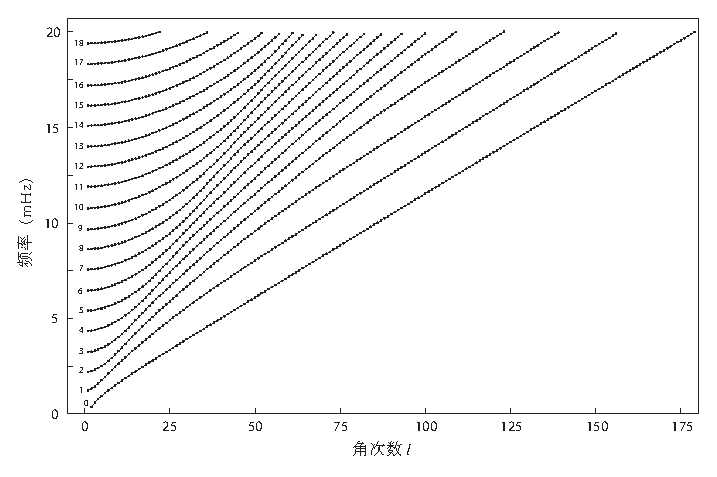
\includegraphics{../figures/chap08/fig03.eps}}
\end{center}
\caption[tormodefreqs]{\label{fig:tormodefreqs}
各向同性~PREM~模型的地幔环型振荡~${}_n{\rm T}_l$~的频散图。图中绘出了低于~20 mHz~的可观测的本征频率~${}_n\omega_l^{\rm T}\hspace{-0.2 mm}/2\pi$~随球谐函数次数~$l$~的变化。径向阶数~$n$~相同的模式由直线相连。
}
\end{figure}
这种方程组的一个基本性质就是本征函数~$\Wnl$~的径向节点数目与径向阶数~$n$相等;这在专业术语上叫做~Sturm~振荡定理。
\index{Sturm's theorem}%
由于这个原因,基阶分支上的所有环型模式在地幔~$b\leq r\leq s$~中均没有节点,而第~$n$~个径向高阶分支的所有模式均有~$n$~个节点。对于~$l=1$,刚体地幔的三重模式在习惯上标记为~${}_0{\rm T}_1$,因而频率最低的非平凡模式是一阶径向高阶模式~${}_1{\rm T}_1$,它有一个径向节点。

对于固体内核的环型模式,下方的边界条件被径向本征函数~$W$、 $T$~在原点~$r=0$~处必须是确定的所取代。在实践中,可以视地球在~$0\leq r\leq\varepsilon$~范围内的一个小部分为均匀球,并利用均匀球的解析解~(\ref{eq:8.Whomsph})--(\ref{eq:8.Thomsph})~作为球心附近的初始值~$W(\varepsilon)$、 $T(\varepsilon)$。积分到内核边界~$r=c$,在那里检视牵引力~$T(c)$~来确定本征频率~$\om$。SNREI~地球的内核环型振荡本质上没有意义,因为它们既不能被地壳或上地幔中的地震所激发,也不会被地表的地震仪观测到。事实上,这些模式一般被认为如此的模糊不清,以致于地震学家们还没有一个都能接受的类似于~${}_n{\rm T}_l$~的符号来表示它们。我们将其表示为~${}_n{\rm C}_l$,其中~$n=0,1,2,\ldots$~是径向阶数。一阶方程组~(\ref{eq:8.tor1})--(\ref{eq:8.tor2})~沿半径增加方向的积分是一个数值上稳定的过程,可以用标准算法来完成。由~Freeman Gilbert、Guy Masters~和~John Woodhouse~
合作开发的广为应用的~{\tt MINEOS\/}~和~{\tt OBANI\/}~程序中,
\index{OBANI@\texttt{OBANI}}%
\index{MINEOS@\texttt{MINEOS}}%
利用了可变阶数、可变步长的~Runge-Kutta~方法来控制积分的精度。对于许多模式,径向本征函数~$W$~和~$T$~在等价的~SH~体波折返点以下呈准指数衰减;在这些情形下,可以使用第~\ref{12.sec.asytor}~节中所讨论的瞬逝型~JWKB~表达式在半径更大的地方开始积分,从而节省时间。Sturm~定理使得能够通过计数测试本征函数~$W$~的径向节点数目来计算~$\om$~的两个测试值之间的本征频率个数。这使得~$T(s)$~或~$T(c)$~的所有的根都能够用上下限括住;一旦上下限建立起来,就能够基于二分法万无一失地收敛到本征频率。能量均分关系~$\om^2\sT=\sV_{\mu}$~可以用来检验最终的计算精度。
\index{numerical integration!toroidal modes|)}%

%\subsection{Toroidal-mode menagerie}
\subsection{环型模式展示}
\label{sec:8.torfigs}

\begin{figure}[!b]
\begin{center}
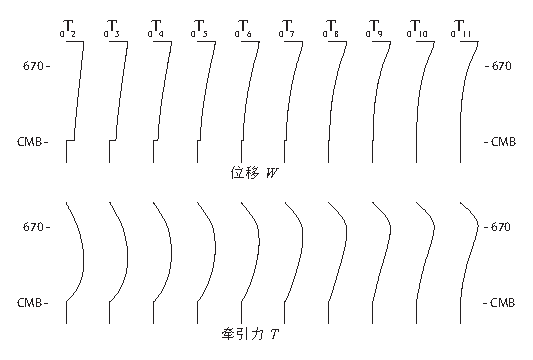
\includegraphics{../figures/chap08/fig04.eps}
\end{center}
\caption[Lovemodes]{\label{fig:Lovemodes}
前~10~个基阶环型模式的位移~${}_0W_l$ ({\em 上\/})~和相应的牵引力${}_0T_l$ ({\em 下\/})。纵轴是地表以下的深度;图中标明了~670 km~不连续面和核幔边界(CMB)的位置。
}
\end{figure}
在本节的最后,我们将对地球环型振荡的主要特征简要地做一个定性的观察。图~\ref{fig:tormodefreqs}~显示了各向同性初步参考地球模型的可观测的地幔环型模式的本征频率~${}_n\omega_l$~随角次数~$l$~的变化。图中每个频散分支~$n=0,1,2,\ldots$~上的模式用直线相连;这种形式的图称为{\em 频散图\/}。
\index{dispersion diagram!toroidal}%
\begin{figure}[!t]
\begin{center}
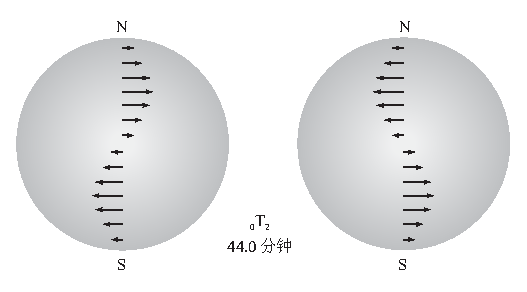
\includegraphics{../figures/chap08/fig05.eps}
\end{center}
\caption[0T2displacements]{\label{fig:0T2}
环型模式~${}_0{\rm T}_2$~的地表位移图像。图中显示了~$m=0$~的单重模式振荡周期的两个极端情形。北极($\theta=0$)和南极($\theta=\pi$)分别用~N~和~S~表示。
}
\end{figure}
\begin{figure}[!b]
\begin{center}
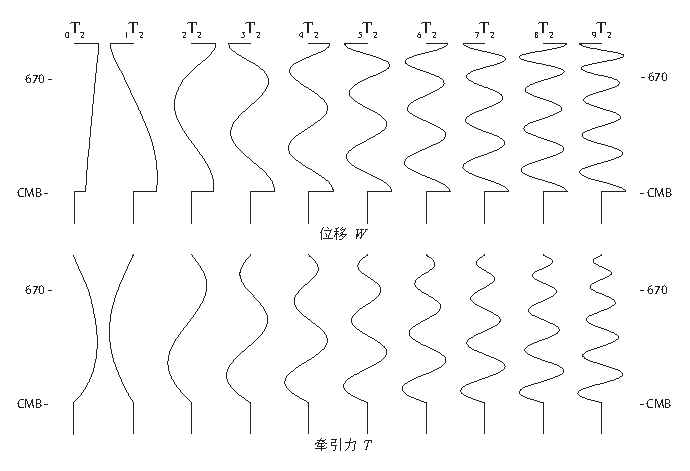
\includegraphics{../figures/chap08/fig06.eps}
\end{center}
\caption[deg2modes]{\label{fig:deg2modes}
前~10~个二次环型模式的位移~${}_nW_2$ ({\em 上图\/})~和相应的牵引力~${}_nT_2$ ({\em 下图\/})。纵轴是地表以下的深度;图中标明了~670 km~不连续面和核幔边界(CMB)的位置。
}
\end{figure}
以图中所示的分辨度,通过拟合~1975~年以后的自由振荡和走时数据所得到的任何~SNREI~地球模型,其频散图都会与~PREM~的难以区分。模型的鉴别是根据以~$\mu$Hz~而非~mHz~为单位的观测频率残差。

\begin{figure}[!t]
\begin{center}
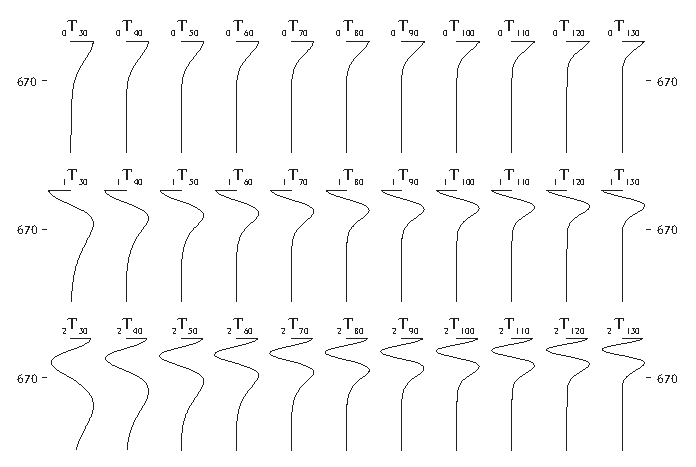
\includegraphics{../figures/chap08/fig07.eps}
\end{center}
\caption[Lovemodes2]{\label{fig:Lovemodes2}
与勒夫波等价的基阶(上排),径向一阶(中排)和径向二阶(下排)分支的本征函数~${}_0W_l$,${}_1W_l$~和~${}_2W_l$。纵轴从地表延伸到~1500 km~深度;图中标明了~670 km~不连续面的位置。
}
\end{figure}

基阶模式位移本征函数~${}_0W_2,\ldots,{}_0W_{11}$~和相应的牵引力~${}_0T_2,\ldots,{}_0T_{11}$~的径向变化如图~\ref{fig:Lovemodes}~所示。最低频的环型模式为~${}_0{\rm T}_2$~五重模式,其简并周期为~44.0~分钟。
\index{fundamental mode!toroidal}%
该振荡直到~1989~年的~Macquarie Rise~走滑大地震~($M_0=2\times10^{21}~{\rm N}\,{\rm m}$)~才首次被明确地探测到~(Widmer, Z\"{u}rn \& Masters 1992)。 \nocite{widmer&zurn92a}。
\index{Macquarie Rise 1989 earthquake}%
如图~\ref{fig:0T2}~所示,$m=0$~的单重模式有一个相应的矢量位移,其形式为~$\bs=-(15/8\pi)^{1/2}
W(r)\sin\theta\cos\theta\,\bphih$,对应于地球的剪切或扭转,即当南半球逆时针移动时,北半球顺时针移动,反之亦然。图~\ref{fig:deg2modes}~显示了次数~($l=2$)~的基阶及其后的九个径向高阶模式的位移~${}_0W_2,\ldots,{}_9W_2$~和牵引力~${}_0T_2,\ldots,{}_9T_2$。很明显${}_nW_2$~在地幔中有~$n$~个径向节点,与~Sturm~定理一致,且~${}_nT_2$~在核幔边界~$r=b$~和海底面~$r=s$~处均为零;这是地幔环型本征解的决定属性。

\begin{figure}[!t]
\begin{center}
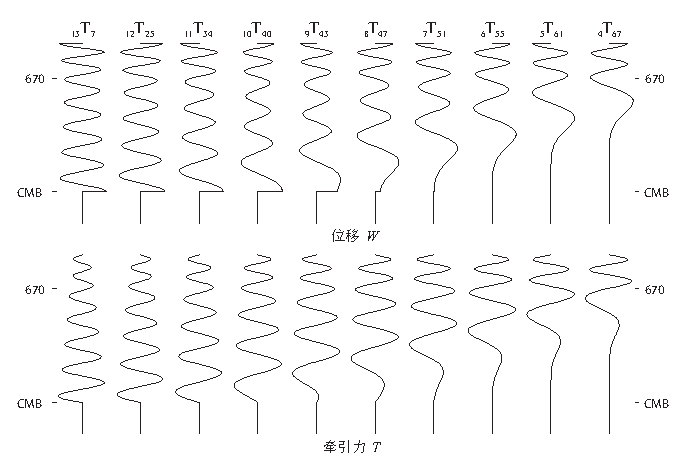
\includegraphics{../figures/chap08/fig08.eps}
\end{center}
\caption[S&ScSmodes]{\label{fig:S&ScSmodes}
沿频率为常数~${}_n\omega_l/2\pi\approx 14$ mHz~的一条直线上的模式的位移~${}_nW_l$~({\em 上排\/})~和相应牵引力~${}_nT_l$~({\em 下排\/}),显示了在~$n\approx l/4$~时~${\rm ScS}_{\rm SH}$-波的等价模式与~SH-波的等价模式之间的过渡。纵轴是地表以下的深度;图中标明了~670 km~不连续面和核幔边界(CMB)的位置。
}
\end{figure}
图~\ref{fig:Lovemodes2}~显示了基阶和前两个径向高阶分支的几个频率较高的环型模式的本征函数~${}_0W_l$、${}_1W_l$~和~${}_2W_l$。沿每一个径向阶数~$n$~不变的分支,随着角次数~$l$~和频率~${}_n\omega_l$~的增加,位移~${}_nW_l$~穿透地幔的深度越来越小。由于下地幔几乎不参与振荡,其性质显然不会对本征频率有很强的影响;在第~9~章中我们会对这种深度“敏感性”做一个更定量的检视。在~$l\gg 1$~的极限下,像${}_0{\rm T}_l,~{}_1{\rm T}_l,~{}_2{\rm T}_l$~这些模式对应于基阶和高阶{\em 勒夫面波\/},
\index{Love wave}%
\index{surface wave!Love}%
\index{mode!surface-wave equivalent}%
或者相当于在上地幔中折返并在海底面反射的~SH~体波的相长干涉。

图~\ref{fig:S&ScSmodes}~展示了有近似相同本征频率~${}_n\omega_l/2\pi\approx 14$ mHz~的一些模式的~$\Wnl$~和~$\Tnl$~的径向变化。其中径向阶数最高的模式,它们的本征频率在频散图中接近纵轴,其振荡位移在整个地幔中振幅大致是均匀的,且对应于在核幔边界和海底面均反射多次的~${\rm ScS}_{\rm SH}$~体波。$l\approx 1$~的相邻环型模式的本征频率间距~${}_{n+1}\om_l-{}_n\om_l$~约等于~$2\pi/\hspace{0.2 mm}T_{\rm ScS}$,其中~$T_{\rm ScS}$~为垂直传播的~${\rm ScS}_{\rm SH}$~波的往返走时。${\rm ScS}_{\rm SH}$~等价频散曲线的斜率或渐近群速度~$d\om/dk\approx{}_n\om_{l+1}
-{}_n\om_l$~在纵坐标附近趋于零。反射波~${\rm ScS}_{\rm SH}$~的等价模式与折返波~SH~的等价模式之间的过渡沿~$\omega/k\approx 2\times 10^{-3}$~rad/s~或相当于~$n\approx l/4$~的斜线发生,每条频散曲线在此均有单一拐点。$n\gg l/4$~的环型模式~${}_n{\rm T}_l$有$d^2\om/dk^2>0$,是~${\rm ScS}_{\rm SH}$~等价模式,而~$n\ll l/4$~的环型模式则有~$d^2\om/dk^2<0$,是~SH~等价模式。在第~12~章中,我们将对高频的地幔环型振荡与传播的~${\rm ScS}_{\rm SH}$~和~SH~体波之间的渐近对应关系做更系统的~JWKB~分析。
\index{mode!toroidal|)}%
\index{toroidal mode|)}%

%\section{Spheroidal Oscillations}
\section{球型振荡}
\index{mode!spheroidal|(}%
\index{spheroidal mode|(}%
\label{section:8.spheroidaloscillations}

SNREI~地球模型的球型振荡有如下形式的相应本征函数
\index{eigenfunction!spheroidal}%
\eq \label{eq:8.spherdis}
\bs=U\bP_{lm}+V\bB_{lm},\qquad\brh\cdot\bT=
R\bP_{lm}+S\bB_{lm},
\en
其中~$\bP_{lm}=\brh\ylm$,$\bB_{lm}=k^{-1}[\bthetah\p_{\theta}
+\bphih(\sin\theta)^{-1}\p_{\phi}]\ylm$。径向和切向牵引标量~$R$和$S$~与相应的位移标量~$U$和$V$~之间的关系为\vspace{-0.6 mm}
$R=(\kappa+\fourthirds\mu)\dU
+(\kappa-\twothirds\mu)r^{-1}(2U-\sqL V)$,
$S=\mu(\dV-r^{-1}V+\sqL r^{-1}U)$。相应的重力势函数微扰为~$\phi=P\ylm$,其中~$P$~通过~(\ref{8.Pexplicit})~式用~$U$~和~$V$~以显式给定。为方便起见,我们定义一个辅助函数
\eq
B=\dP+4\pi G\rho\hspace{0.2 mm}U+(l+1)r^{-1}P,
\label{eq:8.K}
\en
根据边界条件~(\ref{eq:8.ap}),该函数在地球表面~$r=a$~处为零。本征频率~$\om$~和六个径向标量~$U$、$V$、$R$、$S$、$P$和$B$~依赖于径向阶数~$n$~和角次数~$l$,但与方位角级数~$m$~无关。角次数~$l=0$~的球型振荡具有纯径向的位移和牵引力矢量,因为切向的矢量球谐函数~$\bB_{00}$~为零;这些模式被称为{\em 径向模式\/}。
\index{mode!radial}%
\index{radial mode}%


%\subsection{Spheroidal energy}
\subsection{球型能量}
\index{energy!spheroidal mode|(}%
\index{spheroidal mode energy|(}%
\label{section:spheroidalenergy}

将表达式~(\ref{eq:8.spherdis})~代入~(\ref{eq:8.kineticenergy})~和~(\ref{eq:8.bulkenergy})--(\ref{eq:8.gravenergy})~中,可以得到球型振荡的动能与弹性-重力势能之和
\eq \label{8.TOTSPHEN}
\sE=\half(\om^2\sT+\sV_{\kappa}+\sV_{\mu}+\sV_{\rm g}),
\en
其中
\index{energy!kinetic}%
\index{kinetic energy}%
\index{potential energy}%
\index{energy!potential}%
\eq
\sT=\int_0^a\rho(U^2+V^2)\,r^2dr,
\label{eq:8.sTs}
\en
\index{energy!bulk}%
\index{bulk energy}%
\eq
\sV_{\kappa}=\int_0^a\kappa(\dU+2r^{-1}U-\sqL r^{-1}V)^2\,r^2dr,
\label{eq:8.Vbulk}
\en
\index{shear energy}%
\index{energy!shear}%
\eqa
\lefteqn{\sV_{\mu}=\int_0^a\mu\hspace{0.3 mm}[\third(2\dU
-2r^{-1}U+\sqL r^{-1}V)^2} \nonumber \\
&&\mbox{}+(\dV-r^{-1}V+\sqL r^{-1}U)^2
+(\sqL^2-2)r^{-2}V^2]\,r^2dr,
\ena
\index{energy!gravitational}%
\index{gravitational energy}%
\eqa \label{eq:8.Vgrav}
\lefteqn{\sV_{\rm g}=
\int_0^a\rho\hspace{0.3 mm}[U\dP+\sqL r^{-1}VP
+4\pi G\rho\hspace{0.2 mm}U^2} \nonumber \\
&&\mbox{}\qquad\qquad-2gr^{-1}U(2U-\sqL V)]\,r^2dr.
\ena
能量~$\sE$~也可以用球型拉格朗日量密度~$L_{\rm S}$~表示成~(\ref{8.torEL})~的形式。球型模式的瑞利商为
\index{Rayleigh quotient!spheroidal}%
\eq \label{8.spherRayquo}
\om^2=\frac{\sV_{\kappa}+\sV_{\mu}+\sV_{\rm g}}{\sT}.
\en
根据我们所采用的归一化,$\sT=1$,能量均分关系~(\ref{8.spherRayquo})~成为
\index{energy equipartition}%
\index{equipartition relation}%
\eq \label{8.fracpot}
f_{\kappa}+f_{\mu}+f_{\rm g}=1,
\en
这里我们定义了三个无量纲量
\eq
f_{\kappa}=\om^{-2}\sV_{\kappa},\qquad f_{\mu}
=\om^{-2}\sV_{\mu},\qquad f_{\rm g}=\om^{-2}\sV_{\rm g}.
\en
显然,可以将$f_{\kappa}$、$f_{\mu}$~和~$f_{\rm g}$~解释为一个本征频率为~$\om \not= 0$~的非平凡模式的{\em 压缩,剪切\/} 和 {\em 重力\/}的部分能量。
\index{fractional energy}%
\index{energy!fractional}%
由于重力势能~$\sV_{\rm g}$~的符号正负均有可能,所以“部分”一词在这里的必须以更广泛的含义来理解。环型模式没有压缩和重力势能;其所有的能量都在剪切势能中,故~$f_{\mu}=1$。
\index{energy!spheroidal mode|)}%
\index{spheroidal mode energy|)}%


\renewcommand{\thesubsection}{$\!\!\!\raise1.3ex\hbox{$\star$}\!\!$
\arabic{chapter}.\arabic{section}.\arabic{subsection}}
%\subsection{Trivial modes}
\subsection{平凡模式}
\index{mode!trivial|(}%
\index{trivial mode!spheroidal|(}%
\renewcommand{\thesubsection}{\arabic{chapter}.\arabic{section}.\arabic{subsection}}

在第~8.7.2~节中,我们已经看到平凡环型多重模式~${}_0{\rm T}_1$~对应于内核和地幔的刚体旋转。同样有一个平凡球型多重模式~${}_0{\rm S}_1$,它提供了刚体平动的三个自由度。
\index{mode!rigid-body}%
\index{rigid-body mode!spheroidal}%
这个~$l=1$~的零频“模式”的未归一化位移本征函数为~$U=1$~和~$V=\sqrt{2}$;相应的牵引力为零,即~$R=0$~和~$S=0$,且重力势函数微扰是纯平流的:$P=-g$,因而~$B=0$。$m=0$~的单态模式的未归一化矢量位移~${}_0\bs_{10}=\bP_{10}+\sqrt{2}\,\bB_{10}$~为
\eq
{}_0\bs_{10}=(3/4\pi)^{1/2}(\brh\cos\theta
-\bthetah\sin\theta)=(3/4\pi)^{1/2}\bzh,
\en
该式表示的是地球沿~$\bzh$~轴的刚性平动。类似地,${}_0\bs_{1\,-1}=\bP_{1\,-1}+\sqrt{2}\,\bB_{1\,-1}$~和~${}_0\bs_{11}=\bP_{11}+\sqrt{2}\,\bB_{11}$~这两个矢量分别对应于沿~$\bxh$~轴和~$\byh$~轴的平动。需要注意的是,地球的某一部分,比如固态内核,是不可能完全独立于其余部分而平动的。

地转球型模式是不存在的,除非平方~Brunt-V\"{a}is\"{a}l\"{a}~频率在液态外核和海洋~$\earth_{\rm F}$~的整体或一部分中为零时,即~$N^2=0$。
\index{geostrophic mode}%
\index{mode!geostrophic}%
在那种情况下,会有绝热位移局限于中性分层液态区域内部的零频模式存在。
\index{neutral stability}%
\index{stability!neutral}%
任何~$N^2=0$~的地方,满足~$\bdel\cdot(\rho\hspace{0.3 mm}\bs)=0$,或等效地满足
\eq \label{8.Nsqrel}
V=(k\rho r)^{-1}\frac{d}{dr}(\rho r^2 U),
\en
的任何位移都是地转球型模式的本征函数,对应的本征频率为~$\om=0$。(\ref{8.Nsqrel})~式中的径向位移~$U$~在中性分层区域外~$U=0$~的约束下可以任意选择;如果在~$\earth_{\rm F}$~中处处都有~$N^2=0$,那么~$U$~必须在固-液边界~$r=d_{\rm FS}$~上为零。相应的牵引力为纯重力的,即~$R=\rho gU$~和~$S=0$,且势函数微扰为零:即$P=0$,因而~$B=4\pi G\rho\hspace{0.2 mm}U$。对所有角次数~$l>0$,都有一个包含无穷多个这种地转球型模式的家族;这些模式的存在归因于一个事实:即可以将~$\earth_{\rm F}$~中任何中性分层区域翻转而并不改变地球的弹性-重力势能。
\index{mode!trivial|)}%
\index{trivial mode!spheroidal|)}%

%\subsection{First-order radial equations}
\subsection{一阶径向方程}
\index{radial equations!spheroidal mode|(}%

球型模式所满足的三个二阶微分方程~(\ref{eq:8.U})--(\ref{eq:8.V})~和~(\ref{eq:8.P})~可以写成关于~$U$、$V$、$P$、$R$、$S$~和~$B$~的六个耦合一阶方程组的形式:
\eqa \label{eq:8.foU}
\lefteqn{\dU=-2(\kappa+\fourthirds\mu)^{-1}(\kappa-\twothirds\mu)r^{-1}U}
\nonumber \\
&&\mbox{}+\sqL(\kappa+\fourthirds\mu)^{-1}(\kappa-\twothirds\mu)r^{-1}V
+(\kappa+\fourthirds\mu)^{-1}R,
\ena
\eq
\dV=-\sqL r^{-1}U+r^{-1}V+\mu^{-1}S, \label{eq:8.foV}
\en
\eq
\dP=-4\pi G\rho\hspace{0.2 mm}U-(l+1)r^{-1\!}P+B, \label{eq:8.foP}
\en
\eqa \label{eq:8.foR}
\lefteqn{\dR=[-\om^{2\!}\rho-4\rho gr^{-1}+12\kappa\mu
(\kappa+\fourthirds\mu)^{-1}r^{-2}]U} \nonumber \\
&&\mbox{}+[\sqL\rho gr^{-1}
-6\sqL\kappa\mu(\kappa+\fourthirds\mu)^{-1}r^{-2}]V \nonumber \\
&&\mbox{}\qquad-4\mu(\kappa+\fourthirds\mu)^{-1}r^{-1}R
+\sqL r^{-1}S \nonumber \\
&&\mbox{}\qquad\qquad-(l+1)\rho r^{-1}P+\rho B,
\ena
\eqa \label{eq:8.foS}
\lefteqn{\dS=[\sqL\rho g r^{-1}
-6\sqL\kappa\mu(\kappa+\fourthirds\mu)^{-1} r^{-2}]U} \nonumber \\
&&\mbox{}-[\om^{2\!}\rho+2\mu r^{-2}
-4\sqL^2\mu(\kappa+\third\mu)
(\kappa+\fourthirds\mu)^{-1}r^{-2}]V \nonumber \\
&&\mbox{}\qquad-\sqL(\kappa-\twothirds\mu)
(\kappa+\fourthirds\mu)^{-1}r^{-1}R 
-3r^{-1}S
+\sqL\rho r^{-1}P,
\ena
\eq
\dot{B}=-4\pi G(l+1)\rho r^{-1}U+4\pi G\sqL\rho r^{-1}V+(l-1)r^{-1}B.
\label{eq:8.foK}
\en
(\ref{eq:8.foU})--(\ref{eq:8.foK})~中所有的因变量在~$0\leq r\leq a$~上处处连续,只有切向位移~$V$~在固-液边界可以有不连续跃变:即在$r=d_{\rm SS}$~上$[V]^+_-=0$;在~$r=d_{\rm SS}$~和~$r=d_{\rm FS}$~上~$[U]^+_-=0$,$[P]^+_-=0$,$[R]^+_-=0$,$[S]^+_-=0$,和$[B]^+_-=0$。
\index{boundary conditions!spheroidal}%
(\ref{eq:8.K})~式中特意引入的~$B$~是要使在地球表面有齐次边界条件:
\eq \label{eq:8.bfoa}
R=S=0\quad\mbox{and}\quad B=0\quad\mbox{当 $r=a$时.}
\en
另外,剪切牵引力在滑动界面上必须为零:
\eq \label{8.Fried}
S=0\quad\mbox{当 $r=d_{\rm FS}$时.}
\en
方程组~(\ref{eq:8.foU})--(\ref{eq:8.foK})~不依赖于模型参数的径向导数~$\dot{\kappa}$、$\dot{\mu}$~和~$\dot{\rho}$;这使其适宜于数值积分。

%\subsection{Fluid regions}
\subsection{液态区域}
\index{radial equations!fluid regions|(}%

在地球的液态区域内刚度~$\mu$~为零,因此剪切牵引力及其径向导数为零:即在~$\earth_{\rm F}$~中~$S=0$,$\dS=0$。此时,(\ref{eq:8.foS})~可以写成一个用~$U$、$P$和$R$~来表示切向位移~$V$~的代数方程:
\eq
V=\frac{\sqL r^{-1}(\rho gU+\rho P-R)}{\om^{2\!}\rho}. \label{eq:8.Vfl}
\en
利用该结果我们可以在剩下四个径向本征函数~$U$、$P$、$R$~和~$B$~所满足的方程中消去~$V$:
\eqa \label{eq:8.Ufl}
\lefteqn{\dU=(\om^{-2}\sqL^2gr^{-2}-2r^{-1})U
+(\kappa^{-1}-\om^{-2}\sqL^2\rho^{-1}r^{-2})R} \nonumber \\
&&\mbox{}+\om^{-2}\sqL^2r^{-2}P,
\ena
\eq
\dP=-4\pi G\rho\hspace{0.2 mm}U-(l+1)r^{-1\!}P+B,
\en
\eqa
\lefteqn{\dR=(-\om^{2\!}\rho-4\rho g r^{-1}+\om^{-2}\sqL^2\rho g^2r^{-2})U
-\om^{-2}\sqL^2gr^{-2}R} \nonumber \\
&&\mbox{}+[\om^{-2}\sqL^2\rho gr^{-2}-(l+1)\rho r^{-1}]P+\rho B,
\ena
\eqa
\lefteqn{\dot{B}=4\pi G\rho[\om^{-2}\sqL^2gr^{-2}-(l+1)r^{-1}]U
-4\pi G\om^{-2}\sqL^2r^{-2}R} \nonumber \\
&&\mbox{}+4\pi G\om^{-2}\sqL^2\rho r^{-2}P+(l-1)r^{-1}B.
\label{eq:8.Kfl}
\ena
方程组~(\ref{eq:8.Vfl})--(\ref{eq:8.Kfl})~对~$\dot{\kappa}$~和~$\dot{\rho}$没有任何依赖性,这使其成为地球的简正模式地震学中首选的线性化流体动力学方程组。研究太阳和其他恒星的绝热振荡的天体物理学家和太阳地震学家们通常要求解一个等价的四元方程组,
\index{star}%
\index{Sun}%
\index{helioseismology}%
而欧拉压强微扰~$p^{\rm E1}=-R+\rho g\hspace{0.2 mm}U$~是其中使用的因变量之一,且模型是用密度~$\rho$、声速~$\alpha=(\kappa/\hspace{-0.3 mm}\rho)^{1/2}$和~Brunt-V\"{a}is\"{a}l\"{a}~或浮力频率~$N$~给定的(Cox \citeyear{cox80}; Unno, Osaki, Ando, Saio \& Shibahashi \citeyear{unno&al89})。
\index{radial equations!fluid regions|)}%

%\subsection{Radial oscillations}
\subsection{径向振荡}
\index{radial equations!radial mode|(}%
\index{radial mode|(}%
\index{mode!radial|(}%

径向模式有~$V=0$~和~$S=0$,需要单独考虑。相关的重力势函数微扰~$P$~可以用径向位移~$U$~表示为
\eq
\label{8.radP}
P(r)=\left\{
\begin{array}{ll}
\displaystyle{4\pi G\int_r^a\rho'U'\,dr'} &
\quad\mbox{若 $0\leq r\leq a$} \\
0 & \quad\mbox{若 $r\geq a$.}
\end{array}\right.
\en
这是方程~(\ref{8.Pexplicit})--(\ref{8.Pexplicit2})~的一个特例。因为地球模型仍为球对称,且总质量保持不变,所以外部势函数微扰为零。利用显式表达式~(\ref{8.radP}),我们可以将$U$、$R$、$P$~和~$B$~所满足的四个一阶方程简化为径向位移~$U$~和牵引力~$R$~的两个一阶方程:
\eq
\dU=-2(\kappa+\fourthirds\mu)^{-1}(\kappa-\twothirds\mu)r^{-1}U
+(\kappa+\fourthirds\mu)^{-1}R,
\label{eq:8.Urad}
\en
\vspace{-3.0 mm}
\eqa
\lefteqn{\dR=[-\om^{2\!}\rho-4\rho g r^{-1}+12\kappa\mu
(\kappa+\fourthirds\mu)^{-1}r^{-2}]U} \nonumber \\
&&\mbox{}-4\mu(\kappa+\fourthirds\mu)^{-1}r^{-1}R.
\label{eq:8.Rrad}
\ena
方程~(\ref{eq:8.Urad})--(\ref{eq:8.Rrad})~与相应的运动学和动力学边界条件:即在$r=d$时~$[U]^+_-=0$,$[R]^+_-=0$以及
\index{boundary conditions!radial}%
\eq \label{8.radbc}
R=0\quad\mbox{当 $r=a$时,}
\en
一起构成一个~Sturm--Liouville~本征值问题。
\index{Sturm-Liouville problem}%
因此,位移本征函数~${}_nU_0$~的径向节点数与径向阶数~$n$相等。

径向模式的作用量~(\ref{8.spheract})~式简化为
\index{action!radial modes}%
\index{action}%
\eq \label{8.RADACT}
\sI_{\rm R}=\int_0^aL_{\rm R}(U,\dU)\,r^2dr,
\en
其中
\index{Lagrangian density!radial modes}%
\eqa \label{8.radI}
\lefteqn{
L_{\rm R}=\half[\om^{2\!}\rho\hspace{0.2 mm}
U^2-\kappa(\dU+2r^{-1}U)^2} \nonumber \\
&&\mbox{}\qquad\qquad-\fourthirds\mu(\dU-r^{-1}U)^2+4\rho gr^{-1}U^2].
\ena
瑞利原理表明,对于任一可容许变量~$\delta U$,当且仅当~$U$~是本征频率为~$\omega$~的径向模式的本征函数时,$\delta\sI_{\rm R}=0$。欧拉-拉格朗日方程
\index{Euler-Lagrange equations!radial modes}%
\eq \label{8.RADEL}
\p_UL_{\rm R}-
r^{-2}\frac{d}{dr}(r^2\p_{\dot{U}}L_{\rm R})=0
\en
以及相应的变分边界条件:即当$r=d$时,$[\p_{\dot{U}}L_{\rm R}]^+_-=0$和当$r=a$时,~$\p_{\dot{U}}L_{\rm R}=0$,与~Sturm--Liouville~本征值问题~(\ref{eq:8.Urad})--(\ref{8.radbc})是等价的。

径向模式的压缩、剪切和重力势能~(\ref{eq:8.Vbulk})--(\ref{eq:8.Vgrav})~亦可简化为
\index{energy!bulk}%
\index{bulk energy}%
\eq \label{8.radbulk}
\sV_{\kappa}=\int_0^a\kappa(\dU+2r^{-1}U)^2\,r^2dr,
\en
\index{energy!shear}%
\index{shear energy}%
\eq
\sV_{\mu}=\fourthirds\int_0^a
\mu(\dU-r^{-1}U)^2\,r^2dr,
\en
\index{gravitational energy}%
\index{energy!gravitational}%
\eq
\label{8.radgrav}
\sV_{\rm g}=-4\int_0^a\rho(gr^{-1}U^2)\,r^2dr.
\en
重力势能~$\sV_{\rm g}$~的负值表明对径向模式的{\em 自重力失稳效应\/}。
\index{stability!gravitational}%
\index{gravitational stability}%
其物理原因是显而易见的:任何向球心移动的球壳都会感受到加大的重力作用。如果不可压缩性和刚性所提供的恢复力不足,使得~$\sV_{\kappa}+\sV_{\mu}+
\sV_{\rm g}\leq 0$,那么整个构形会产生{\em 重力坍缩\/}。
\index{gravitational collapse}%
\index{radial mode|)}%
\index{mode!radial|)}%
\index{radial equations!radial mode|)}%

\renewcommand{\thesubsection}{$\!\!\!\raise1.3ex\hbox{$\star$}\!\!$
\arabic{chapter}.\arabic{section}.\arabic{subsection}}
%\subsection{Neglect of self-gravitation}
\subsection{自重力的忽略}
\index{self-gravitation!neglect of|(}%
\index{radial equations!non-gravitating|(}%
\renewcommand{\thesubsection}{\arabic{chapter}.\arabic{section}.\arabic{subsection}}

对于周期小于约~30~秒的振荡,地球的自重力与其弹性不可压缩性和刚性相比,在恢复力上所起的作用可以忽略不计。因而可以令引力常数~$G$、重力加速度~$g$以及方程~(\ref{eq:8.foU})--(\ref{eq:8.foK})~中的重力势函数微扰~$P$~和~$B$~为零,使地球的固态区域~$\earth_{\rm S}$~所满足的六个一阶微分方程被一组四个方程代替:
\eqa \label{eq:8.igU}
\lefteqn{\dU=-2(\kappa+\fourthirds\mu)^{-1}(\kappa-\twothirds\mu)
r^{-1}U} \nonumber \\
&&\mbox{}+\sqL(\kappa+\fourthirds\mu)^{-1}(\kappa-\twothirds\mu)
r^{-1}V
+(\kappa+\fourthirds\mu)^{-1}R,
\ena
\eq
\dV=-\sqL r^{-1}U+r^{-1}V+\mu^{-1}S, \label{eq:8.igV}
\en
\eqa \label{eq:8.igR}
\lefteqn{\dR=[-\om^{2\!}\rho+12\kappa\mu
(\kappa+\fourthirds\mu)^{-1}r^{-2}]U} \nonumber \\
&&\mbox{}-6\sqL \kappa\mu(\kappa+\fourthirds\mu)^{-1}r^{-2}V \nonumber \\
&&\mbox{}\qquad-4\mu(\kappa+\fourthirds\mu)^{-1}r^{-1}R
+\sqL r^{-1}S,
\ena
\eqa \label{eq:8.igS}
\lefteqn{\dS=-6\sqL \kappa\mu(\kappa+\fourthirds\mu)^{-1}
r^{-2}U} \nonumber \\
&&\mbox{}-[\om^{2\!}\rho+2\mu r^{-2}-4\sqL^2\mu(\kappa+\third\mu)
(\kappa+\fourthirds\mu)^{-1}r^{-2}]V \nonumber \\
&&\mbox{}\qquad-\sqL (\kappa-\twothirds\mu)
(\kappa+\fourthirds\mu)^{-1}r^{-1}R-3r^{-1}S.
\ena
在地球的液态区域~$\earth_{\rm F}$,切向位移~(\ref{eq:8.Vfl})~由~$V=-(\sqL r^{-1}R)/(\om^{2\!}\rho)$~给定,同时我们得到径向位移~$U$~和牵引力~$R$~的一阶微分方程租:
\eq \label{eq:8.igfU}
\dU=-2r^{-1}U
+(\kappa^{-1}-\om^{-2}\sqL^2\rho^{-1}r^{-2})R,
\en
\eq
\dR=-\om^{2\!}\rho\hspace{0.2 mm}U.
\label{eq:8.igfR}
\en
方程组~(\ref{eq:8.igU})--(\ref{eq:8.igS})~和~(\ref{eq:8.igfU})--(\ref{eq:8.igfR})~必须在当$r=a$时~$R=S=0$的边界条件下来求解。这种无重力近似在数值应用中已经很少使用了,因为在~$\earth_{\rm S}$~中仅需对一组四个而非六个方程积分,以及在~$\earth_{\rm F}$~中只需要对一组两个而非四个方程积分的优势,已经被现代计算机的能力所抵消。在第~\ref{12.sec.JWKBS}~节中,我们将利用这些结果来得到~$\om\rightarrow\infty$~极限下的半解析的~JWKB~本征频率和本征函数。

因重力而存在的振荡,例如我们将在第~8.8.11~节要讨论的,已经从方程组~(\ref{eq:8.igU})--(\ref{eq:8.igS})~和~(\ref{eq:8.igfU})--(\ref{eq:8.igfR})~中消除了。短波长由重力主导的模式可以用一个限制性较弱的近似来研究,其中忽略~$P$、$B$~和~$G$,但保留初始重力加速度~$g$。由此得到稍微复杂一些的方程组,包含在~$\earth_{\rm S}$~中~$U$、$V$、$R$~和~$S$~所满足的四个方程和在~$\earth_{\rm F}$~中~$U$~和~$R$~所满足的两个方程。在这一{\em Cowling近似\/}近似中,方程组~(\ref{eq:8.igfU})--(\ref{eq:8.igfR})~推展为
\index{Cowling approximation}%
\eq \label{8.Cowling1}
\dU=(\om^{-2}\sqL^2gr^{-2}-2r^{-1})U
+(\kappa^{-1}-\om^{-2}\sqL^2\rho^{-1}r^{-2})R,
\en
\eq \label{8.Cowling2}
\dR=(-\om^{2\!}\rho-4\rho g r^{-1}+\om^{-2}\sqL^2\rho g^2r^{-2})U
-\om^{-2}\sqL^2gr^{-2}R.
\en
\index{radial equations!Cowling approximation}%
正如我们在~4.3.5~节中指出的,方程组~(\ref{8.Cowling1})--(\ref{8.Cowling2})~在计算时代到来之前被用来研究太阳和其他恒星的由引力主导~($f_{\rm g}\gg f_{\kappa}$)~和声学主导~($f_{\kappa}\gg f_{\rm g}$)~的振荡。
\index{Sun}%
\index{star}%
\index{self-gravitation!neglect of|)}%
\index{radial equations!spheroidal mode|)}%
\index{radial equations!non-gravitating|)}%

\renewcommand{\thesubsection}{$\!\!\!\raise1.3ex\hbox{$\star$}\!\!$
\arabic{chapter}.\arabic{section}.\arabic{subsection}}
%\subsection{Homogeneous sphere: radial oscillations}
\subsection{均匀球体:径向振荡}
\index{homogeneous sphere!radial modes|(}%
\renewcommand{\thesubsection}{\arabic{chapter}.\arabic{section}.\arabic{subsection}}

一个半径为~$a$、并具有均匀的密度~$\rho$、压缩波波速\vspace{-0.3 mm}
$\alpha=[(\kappa+\fourthirds\mu)/\hspace{-0.3 mm}\rho]^{1/2}$,和剪切波波速~$\beta=(\mu/\hspace{-0.3 mm}\rho)^{1/2}$~的自重力固体球的径向振荡是很容易计算的。这种均匀球内的重力加速度随半径线性变化:即在~$0\leq r\leq a$~内,$g=\fourthirds\pi G\rho r$。联立方程~(\ref{eq:8.Urad})~和~(\ref{eq:8.Rrad})~得到二阶常微分方程:
\eq \label{8.homradeqn}
\ddU+2r^{-1}\dU+(\gamma^2-2r^{-2})U=0,
\en
其中$\gamma^2=(\om^2+\sixteenthirds\pi G\rho)\alpha^{-2}$。我们发现~(\ref{8.homradeqn})~为~$l=1$~次的球贝塞尔方程,其解为:
\eq \label{8.radstart1}
U=j_1(\gamma r).
\en
与位移~(\ref{8.radstart1})~相应的径向牵引力~$R=(\kappa+\fourthirds\mu)
(\dU+2r^{-1}U)-4\mu r^{-1}U$~为
\eq \label{8.radstart2}
R=(\kappa+\fourthirds\mu)\gamma\,j_0(\gamma r)
-4\mu r^{-1}j_1(\gamma r).
\en
自由表面边界条件~$R(a)=0$~意味着
\eq
\cot(\gamma a)=(\gamma a )^{-1}
-\fourth\mu^{-1}(\kappa+\fourthirds\mu)
\gamma a.
\label{eq:8.radroot}
\en
均匀球的径向模式本征频率~${}_n\om_0$~由方程~(\ref{eq:8.radroot})~的根~${}_{\raise-.35ex\hbox{\scriptsize\it n}\!}
\gamma_{\raise-.35ex\hbox{\scriptsize\rm 0}}$~来确定:
\eq \label{eq:8.radroot2}
\om^2=\gamma^2\alpha^2-\sixteenthirds\pi G \rho.
\en
对于液态($\mu=0$)球,这些根直接就是~${}_{\raise-.35ex\hbox{\scriptsize\it n}\!}
\gamma_{\raise-.35ex\hbox{\scriptsize\rm 0}}
=(n+1)\pi\hspace{-0.3 mm}/\hspace{-0.3 mm}a$。对于泊松固体($\kappa=\fivethirds\mu$),
\index{Poisson solid}%
这些根略小一些:${}_{\raise-.35ex\hbox{\scriptsize\rm 0}\!}
\gamma_{\raise-.35ex\hbox{\scriptsize\rm 0}}
=0.82\,\pi\hspace{-0.3 mm}/\hspace{-0.3 mm}a$~和~${}_{\raise-.35ex\hbox{\scriptsize\rm 1}\!}
\gamma_{\raise-.35ex\hbox{\scriptsize\rm 0}}
=1.98\,\pi\hspace{-0.3 mm}/\hspace{-0.3 mm}a$。一个{\em 无自重力\/}($G=0$)的泊松固体球的本征频率满足
\eq \label{8.POISSON}
\cot(\om a/\alpha)=(\om a/\alpha)^{-1}
-\threefourths(\om a/\alpha).
\en
(\ref{8.POISSON})这一结果非常著名——如我们在第一章中指出的, \textcite{poisson29}对它的推导标志着地球自由振荡的理论分析的开端。

自重力的失稳效应表现在~(\ref{eq:8.radroot2})~式中负值的最后一项~$-\sixteenthirds\pi G \rho$~。最不稳定的振荡是基阶模式~${}_0{\rm S}_0$,当不可压缩性和刚度足够小或者密度和半径足够大,以至于
\eq
\alpha<\alpha_{\rm crit}
={}_{\raise-.35ex\hbox{\scriptsize\rm 0}\!}\gamma_0^{-1}
(\sixteenthirds\pi G\rho)^{1/2}
\en
时,其本征频率平方~${}_{\raise-.2ex\hbox{\scriptsize\rm 0}}\om^2_0$~是负的。
对于一个与太阳具有相同半径~($a=696,000$~km)~和平均密度~($\rho=1408$~kg/m${}^3$)~的均匀液态球体,
\index{Sun}%
避免其引力坍缩所需的临界声波速度为~$\alpha_{\rm crit}=278$~km/s。
\index{gravitational collapse}%
对于一个与地球具有相同半径($a=6371$ km)和平均密度~($\rho=5514$~kg/m${}^3$)~的均匀泊松固态球体,其临界波速为~$\alpha_{\rm crit}=\sqrt{3}\,\beta_{\rm crit}=6.18$~km/s。太阳内部实际的声波速度从表面的几乎为零增加到日心的大约~500~km/s,
\index{helioseismology}%
而地球的地幔中实际的压缩波速度从莫霍不连续面下的~8.1~km/s~增加到核幔边界上的~13.7~km/s。在这两个球体内部$\alpha$、$\beta$~和~$\rho$~的分层结构使它们与上述简化的例子相比更能够在径向形变下保持稳定。
\index{homogeneous sphere!radial modes|)}%

\renewcommand{\thesubsection}{$\!\!\!\raise1.3ex\hbox{$\star$}\!\!$
\arabic{chapter}.\arabic{section}.\arabic{subsection}}
%\subsection{Homogeneous sphere: non-radial oscillations}
\subsection{均匀球体:非径向振荡}
\index{homogeneous sphere!spheroidal modes|(}%
\renewcommand{\thesubsection}{\arabic{chapter}.\arabic{section}.\arabic{subsection}}

\textcite{love11},\textcite{pekeris&jarosch58}~以及~\textcite{takeuchi&saito72}~详细地讨论了一个自重力均匀固体球的非径向自由振荡;我们在此仅直接引用他们的结果。径向本征函数方程组~(\ref{eq:8.foU})--(\ref{eq:8.foK})~的三个线性独立的规则解中有两个可以用~$l$~和~$l+1$~次的球贝塞尔函数表示为:
\eq
U=l\xi r^{-1}j_l(\gamma r)-
\zeta\gamma\,j_{l+1}(\gamma r), \label{eq:8.shom1.1}
\en
\eq
V=\sqL\xi r^{-1}j_l(\gamma r)+\sqL \gamma\,j_{l+1}(\gamma r),
\en
\eq
P=-4\pi G\rho\zeta\,j_l(\gamma r),
\en
\eqa
\lefteqn{R=-[(\kappa+\fourthirds\mu)\zeta\gamma^2
+2l(l-1)\mu\xi r^{-2}]j_l(\gamma r)}\nonumber \\
&&\mbox{}-2\mu(2\zeta+\sqL^2)
\gamma r^{-1}j_{l+1}(\gamma r),
\ena
\eqa \lefteqn{
S=\sqL\mu[\gamma^2+2(l-1)\xi r^{-2}]j_l(\gamma r)} \nonumber \\
&&\mbox{}-2\sqL\mu(\zeta+1)\gamma r^{-1}j_{l+1}(\gamma r),
\ena
\eq
B=-4\pi G\rho r^{-1}[\sqL^2-(l+1)\zeta]j_l(\gamma r), \label{eq:8.shom1.6}
\en
其中
\eqa
\lefteqn{\gamma^2=\frac{\om^2}{2\beta^2}
+\frac{\om^2+\sixteenthirds\pi G\rho}{2\alpha^2}} \nonumber \\
&&\mbox{}\pm\frac{1}{2}\left[\left(\frac{\om^2}{\beta^2}
-\frac{\om^2+\sixteenthirds\pi G\rho}{\alpha^2}\right)^{\!2}
+\left(\frac{8\pi G\sqL\rho}{3\alpha\beta}\right)^{\!2}\right]^{1/2},
\label{eq:8.kpm}
\ena
\eq
\zeta=\threefourths(\pi G\rho)^{-1}\beta^2(\gamma^2-\om^2\!/\!\beta^2),
\qquad \xi=\zeta-(l+1).
\en
要注意的是,由于定义式~(\ref{eq:8.kpm})~中的~$\pm$~号,(\ref{eq:8.shom1.1})--(\ref{eq:8.shom1.6})~中包含两个解。第三个线性独立的正则解由下面的代数表达式给定
\eq
U=lr^{l-1},
\qquad V=\sqL r^{l-1},
\qquad P=(\om^2-\fourthirds\pi G\rho l)r^l,
\label{eq:8.shom3.1}
\en
\eq
R=2l(l-1)\mu r^{l-2},
\qquad S=2\sqL(l-1)\mu r^{l-2},
\en
\eq
B=[(2l+1)\om^2-\eightthirds\pi Gl(l-1)\rho]r^{l-1}. \label{eq:8.shom3.6}
\en
(\ref{eq:8.shom3.1})--(\ref{eq:8.shom3.6})~式是第~8.8.2~节中讨论的刚体本征解的推广;在~$l=1$、$\om=0$~时只有这个解才满足边界条件~$R=0$、$S=0$、$B=0$。均匀固体球的非平凡本征频率~$\om\not= 0$~由如下行列式方程的根决定
\eq
{\rm det}\left|\begin{array}{ccc}
R_1(a) & R_2(a) & R_3(a) \\
S_1(a) & S_2(a) & S_3(a) \\
B_1(a) & B_2(a) & B_3(a)
\end{array}\right|=0,
\label{eq:8.det}
\en
其中下角标~1、2~和~3~表示三个线性独立解。以上分析假定~(\ref{eq:8.kpm})~的两个根~$\gamma^2$~都是正的;任何重力稳定的泊松固体~($\kappa=\fivethirds\mu$)~球都是满足这个条件的。可以进一步证明,这种球体在径向形变下的重力稳定性也可确保其在非径向形变下的完全稳定性。

一个稳定均匀球最低频的自由振荡是{\em 橄榄球模式\/}~${}_0{\rm S}_2$,
\index{mode!football}%
\index{football mode}%
\index{fundamental mode!spheroidal}%
这样称呼是因为其形状变化介于一个美式橄榄球(或者柠檬,如果你喜欢的话)和一个南瓜之间。对于一个质量和大小与地球相同、且“刚度与钢材一样”(\textcite{love11}~给的数值是~$\mu=8.19\times10^{10}$~Pa)的泊松固体球,这一基阶模式的周期“几乎恰好是~60~分钟”。 数值积分得到的各向同性~PREM~模型~${}_0{\rm S}_2$~模式对应的周期为~53.9~分钟。

对于均匀液态球体,并不像~(\ref{eq:8.kpm})~中定义的两个值,而是只有单一的径向波数~$\gamma$:
\eq \label{8.lastRWneed}
\gamma^2=\frac{\om^2+\sixteenthirds\pi G\rho}{\alpha^2}
-\left(\frac{4\pi G\sqL\rho}{3\om\alpha}\right)^2,
\en
\eq
\zeta=-\threefourths(\pi G\rho)^{-1}\om^2,
\qquad \xi=\zeta-(l+1).
\en
因此,有两个而不是三个线性独立解;二乘二的行列式方程
\eq
{\rm det}\left|\begin{array}{cc}
R_1(a) & R_2(a) \\
B_1(a) & B_2(a)
\end{array}\right|=0
\label{eq:8.detfl}
\en
可简化为~$j_l(\gamma a)=0$。通过二次关系式~(\ref{8.lastRWneed}),该球贝塞尔函数的每一个根~${}_{\raise-.35ex\hbox{\scriptsize\it n}\!}
\gamma_{\raise-.35ex\hbox{\scriptsize\rm l}}a$~既可以确定一个纯实数的本征频率~(${}_n\om_l^2>0$),也可以确定一个纯虚数的本征频率~(${}_n\om_l^2<0$)。实数的本征频率对应于稳定的、声波主导的地震学关注的模式;而虚数的本征频率则反映了均匀可压缩液态球体固有的重力不稳定性,其内部处处均有~$N^2=-\rho g^2\!/\hspace{-0.3 mm}\kappa<0$。不存在~$l=0$~次的这种不稳定的重力模式;均匀液态球体仅有的径向振荡是受重力调节的声波模式,其本征频率由~(\ref{eq:8.radroot})~式给定。

唯一的稳定均匀液态球体是{\em 不可压缩的\/},其~$\kappa=\infty$。
\index{incompressible material}%
这样的球体没有径向模式,也没有高阶模式;对所有次数~$l\geq 1$,只有一个基阶振荡,其本征频率由~Kelvin~爵士的经典公式给定(Thomson \citeyear{kelvin63b}):
\eq
\label{8.Kelvin}
\om^2=\frac{\eightthirds\pi l(l-1)G\rho}{2l+1}.
\en
$l=1$~的特例对应于刚体平动三重模式,其~$\om=0$。最低频的非平凡振荡是橄榄球模式~${}_0{\rm S}_2$,当球体的平均密度与太阳或地球相同时,其周期分别为~47.7~分钟或~94.3~分钟。
\index{Sun}%
\index{homogeneous sphere!spheroidal modes|)}%

%\subsection{Numerical integration}
\subsection{数值积分}
\index{numerical integration!spheroidal modes|(}%
\label{sec:8.arbmodel}

包含固态内核、液态外核、固态地幔和地壳以及液态海洋的接近实际的~SNREI~地球模型的球型模式需要通过数值积分来计算。确定非径向振荡的本征频率~$\om$~以及相应的本征函数~$U$、$V$、$P$、$R$、$S$~和~$B$可以从地球模型的球心以外一点开始积分,以均匀球体的精确解~(\ref{eq:8.shom1.1})--(\ref{eq:8.shom1.6})~和~(\ref{eq:8.shom3.1})--(\ref{eq:8.shom3.6})~作为初始值。由于有三个线性独立的正则初始解,我们必须从起始半径~$r=\varepsilon$~到内核边界~$r=c$~将六个一阶方程~(\ref{eq:8.foU})--(\ref{eq:8.foK})~积分三次。在边界处,这些解会有两个线性独立的组合满足边界条件~$S(c)=0$。与这两个线性组合相对应的连续的量~$U(c)$、$R(c)$、$P(c)$~和~$B(c)$~成为液态外核中的四个一阶方程~(\ref{eq:8.Ufl})--(\ref{eq:8.Kfl})~积分到核幔边界~$r=b$~的初始值。$U(b)$、$R(b)$、$P(b)$~和~$B(b)$~的值与初始值~$V(b)=0$和$S(b)=0$~组成地幔底部的两个线性独立解;第三个容许核幔边界有切向滑动可能性的解是~$U(b)=0$、$V(b)=1$、$P(b)=0$、$R(b)=0$、$S(b)=0$、$B(b)=0$。利用方程组~(\ref{eq:8.foU})--(\ref{eq:8.foK})~将这三个解在地幔和地壳中积分;在积分中的任何固-固界面$r=d_{\rm SS}$处,施加连续性条件~$[U]^+_-=0$、$[V]^+_-=0$、$[P]^+_-=0$、$[R]^+_-=0$、$[S]^+_-=0$~以及~$[B]^+_-=0$。如果地球模型没有海
水层,在自由表面~$r=a$处~将会有三个线性独立解,我们用下角标~1、2~和~3~标记。本征频率~$\omnl$~则为非久期行列式方程~(\ref{eq:8.det})~的根;一旦确定了某个特定的~$\omnl$~值,很容易就能得到与其径向本征函数~$\Unl$、$\Vnl$、$\Pnl$、$\Rnl$、$\Snl$~和~${}_nB_l$~相对应的唯一线性组合。如果存在海水层,那么会有两个线性独立的解满足海底的边界条件~$S(s)=0$。利用方程组~(\ref{eq:8.Ufl})--(\ref{eq:8.Kfl})~将这些解进行积分至自由表面$r=a$,然后用~(\ref{eq:8.detfl})~确定本征频率~$\omnl$。对角次数~$l$~的每一个取值都要分别进行积分和行列式的寻根搜索。本征频率按数值大小排序,从最低频开始,依序赋予径向阶数~$n=0,1,2,\ldots$。与环型模式一样,从距地心更远处开始积分,常常可以节省时间,只要注意积分起始点位于等价的~P-SV~体波射线折返点下方足够远处。径向模式的计算单独进行,从~$r=\varepsilon$~处的均匀球解析解~(\ref{8.radstart1})--(\ref{8.radstart2})~开始,将两个一阶方程~(\ref{eq:8.Urad})--(\ref{eq:8.Rrad})积分,然后寻找~$R(a)$~的根~${}_n\om_0$。
\begin{sidewaysfigure}
\centering
\rotatebox{270}
{
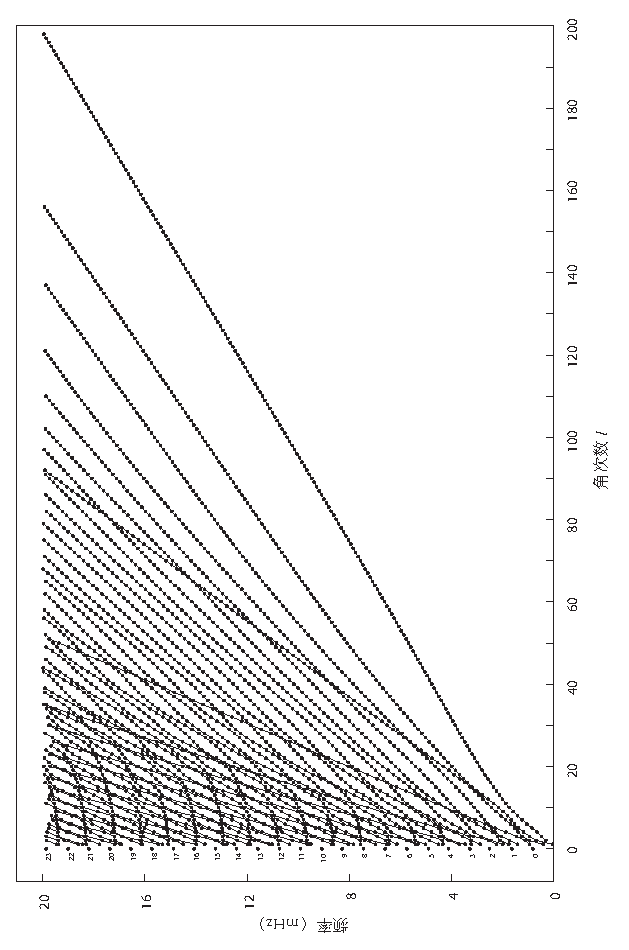
\includegraphics{../figures/chap08/fig09.eps}
}
\caption[sphmodefreqs]{
各向同性~PREM~模型的球型振荡频散图。图中显示了~20 mHz~以下所有以弹性主导的本征频率~${}_n\omega_l^{\rm S}/2\pi$~与球谐函数次数~$l$~的关系。左侧小号的整数标注了径向模式~($l=0$)~本征频率的阶数$n$。更多的细节见图~\ref{fig:sphmodefreqs2}~。
}
\label{fig:sphmodefreqs}
\end{sidewaysfigure}

实用的数值积分算法,如~MINEOS~和~OBANI~中所使用的,
\index{OBANI@\texttt{OBANI}}%
\index{MINEOS@\texttt{MINEOS}}%
在两个重要方面与前面的描述有差别。首先,线性微分方程组~(\ref{eq:8.foU})--(\ref{eq:8.foK})~和~(\ref{eq:8.Ufl})--(\ref{eq:8.Kfl})~是刚性的,
\index{stiff equations}%
因而直接积分即使在中高频率也会导致结果非常不稳定。在~$r=\varepsilon$~处线性独立的初始解随着半径的增大而变得越来越不独立,因而在精度有限的计算机上,它们在数值上变得与一组线性相关的解毫无分别。此时行列式~(\ref{eq:8.det})~和~(\ref{eq:8.detfl})~作为尝试本征频率~$\om$~的函数表现极差。这个困难可以通过分别求解液态区域中~$2\times 4$~解矩阵的~$2\times 2$~子式和固态区域中~$3\times 6$~解矩阵的~$3\times 3$~子式来克服;
\index{minor matrices}%
由此在液态和固态区域中分别得到的~6~维和~20~维子式矢量,除了一个常数系数外,唯一地确定了线性独立解的空间,且不依赖于初始基。Gilbert \& Backus (\citeyear{gilbert&backus66}; \citeyear{gilbert&backus69})~和~\textcite{woodhouse88}~推导并讨论了这些矢量在~$\earth_{\rm S}$和$\earth_{\rm F}$~区域中所满足的一阶常微分方程组,以及相应的固-液边界~$r=d_{\rm FS}$~的连续性条件和自由表面~$r=a$~的边界条件。最后这篇文献还描述了如何用子式矢量重构原来的本征函数~$U$、$V$、$P$、$R$、$S$~和~$B$。对于环型和径向模式,需要将~$W$~和~$T$~或~$U$~和~$R$~的单一的~$1\times 2$~解矢量积分,其子式形式是
退化的。

第二个问题是要确保能够找到所有的本征频率和本征函数。这一问题对于非径向球型模式尤其严重,因为其频谱有许多位置邻近且间隔不规则的本征频率,如我们将在~\ref{sec:8.spherfigs}~节中看到的。直接的穷举搜索需要用极小的频率步长才能保证找到久期行列式所有的根;此外,也无法预先指定合适的频率步长。为了克服这一困难,\textcite{woodhouse88}~推广了~Sturm~定理,只需两次积分便可以通过计数子式矢量的标量积的过零次数来确定~$\om_{\rm min}$~和~$\om_{\rm max}$~两个值之间的本征频率数目。
\index{Sturm's theorem}%
这一惊人的结果使得所有球型模式的本征频率能够被有效地分段限定,然后再用二分法来加以完善,而不必担心有任何遗漏。

%\subsection{Spheroidal-mode menagerie}
\subsection{球型模式展示}
\label{sec:8.spherfigs}

图~\ref{fig:sphmodefreqs}~显示了各向同性~PREM~地球模型弹性为主导的球型振荡的频散图。
\index{dispersion diagram!spheroidal}%
如前所述,本征频率之间的间隔非常不规则;由于这种不规则形,连接每个径向分支~${}_n\om_0\!-\!{}_n\om_1\!-\!{}_n\om_2\cdots$的实线展现出一种“阶梯”的特征。图~\ref{fig:sphmodefreqs2}~以放大的形式展示了球型模式频散图靠近原点的区域;水平比例尺被放大(并在~$l=60$~截断),因而分支之间的密切接触能够看得更清楚。
\begin{sidewaysfigure}
\rotatebox{270}
{
\centering
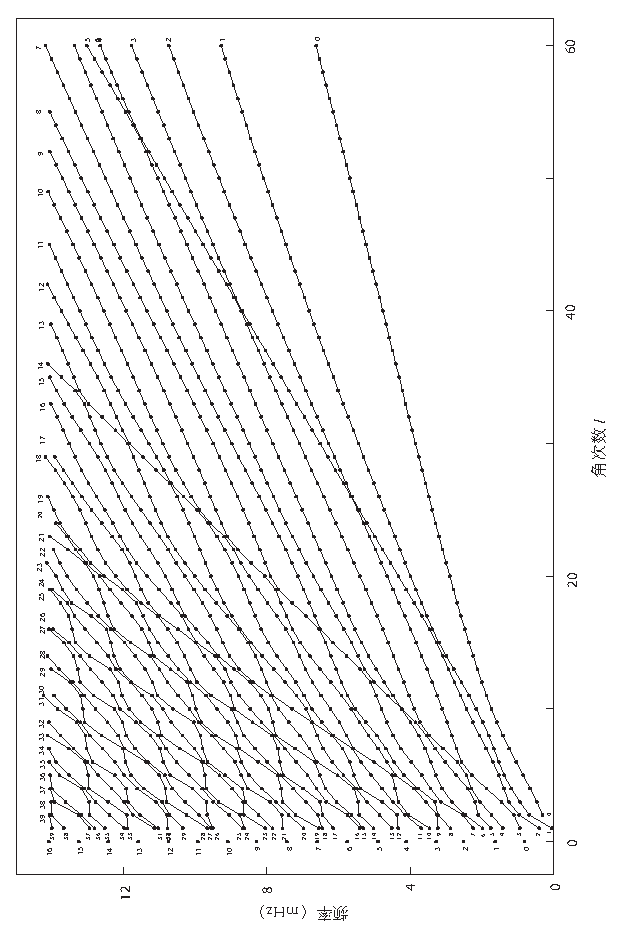
\includegraphics{../figures/chap08/fig10.eps}
}
\caption[sphmodefreqs2]{
图~\ref{fig:sphmodefreqs}中左下角区域的球型模式频散细部图像。最左边的整数~0~至~16~标注了径向模式($l=0$)的本征频率的阶数$n$;重复的整数~0~至~39~在各径向分支的低频端和高频端标注了径向阶数$n$。
}
\label{fig:sphmodefreqs2}
\end{sidewaysfigure}
频散图中左上角部分的高频、径向高阶模式的阶梯特征最为明显。

在图~\ref{fig:sphmodefreqs}~中右侧具有规则间隔的模式~${}_0{\rm S}_l$、${}_1{\rm S}_l$、${}_2{\rm S}_l$~等在~$l\gg 1$~极限下对应于基阶和高阶{\em 瑞利面波\/},或等价于在上地幔中相长干涉的多次反射的~P~和~SV~体波。
\index{Rayleigh wave}%
\index{surface wave!Rayleigh}%
\index{mode!fundamental}%
\index{fundamental mode}%
\index{mode!surface-wave equivalent}%
图~{\ref{fig:fundsphmodes}~展示了几个这种瑞利波等价模式的~${}_0U_l$、${}_1U_l$、${}_2U_l$~和~${}_0V_l$、${}_1V_l$、${}_2V_l$~的径向变化。沿基阶和任一高阶分支,某一模式~${}_0{\rm S}_l$、${}_1{\rm S}_l$ 、${}_2{\rm S}_l$~能够穿透或“感觉到”的地幔的深度随着角次数~$l$~的增加而减小,正如第~\ref{sec:8.torfigs}~节中所讨论的类似的与勒夫波等价的环型模式~${}_0{\rm T}_l$、${}_1{\rm T}_l$、${}_2{\rm T}_l$。基阶瑞利波等价模式的径向位移~${}_0U_l$~没有径向节点,而切向位移~${}_0V_l$~有一个径向节点。在第~11.4~节我们会看到,在地球表面~$r=a$~处,${}_0U_l$~和~${}_0V_l$~的符号
差别暗示了基阶瑞利波{\em 顺进质点运动\/}的特点。
\index{particle motion!Rayleigh-wave}%
\index{prograde particle motion}%

阶数与频率较高且间隔不规则的模式对应于传播路径较陡的、与固态内核和液态外核边界相互作用的~P~和~SV~体波。这些模式有三个截然不同的家族,每一个都表现出较为规则的本征频率~${}_n\om_l$的分布图像;固定~$n$~的频散曲线的阶梯形状源于这三类模式的“规避交叉”现象。
\begin{figure}[!t]
\begin{center}
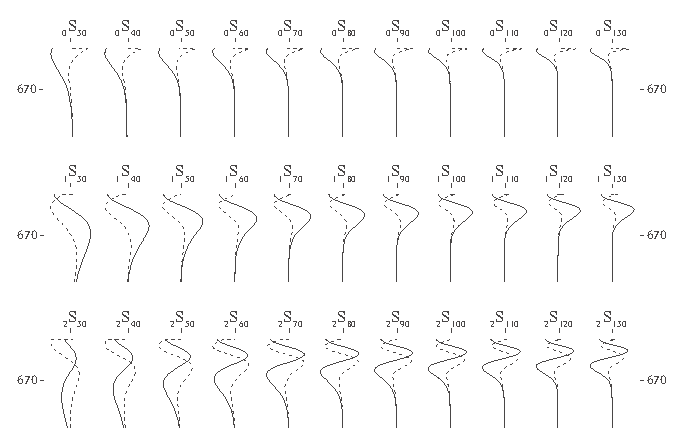
\includegraphics{../figures/chap08/fig11.eps}
\end{center}
\caption[fundsphmodes]{\label{fig:fundsphmodes}
与瑞利波等价的基阶(上排),径向一阶(中排)和径向二阶(下排)分支的本征函数~${}_0U_l$、${}_1U_l$、${}_2U_l$~({\em 实线\/})~和~${}_0V_l$、${}_1V_l$、${}_2V_l$~({\em 点线\/})。纵轴从地表延伸到~1200 km~深度;图中标明了~670 km~不连续面的位置。
}
\end{figure}
将观察者的眼睛贴近图~\ref{fig:sphmodefreqs}~的平面,以近乎平行的视角可以更明显地看清这三类曲线;为清楚起见,我们在图~\ref{fig:threemodes}~中将这三类本征频率分别画出。
\begin{sidewaysfigure}
\centering
\rotatebox{270}
{
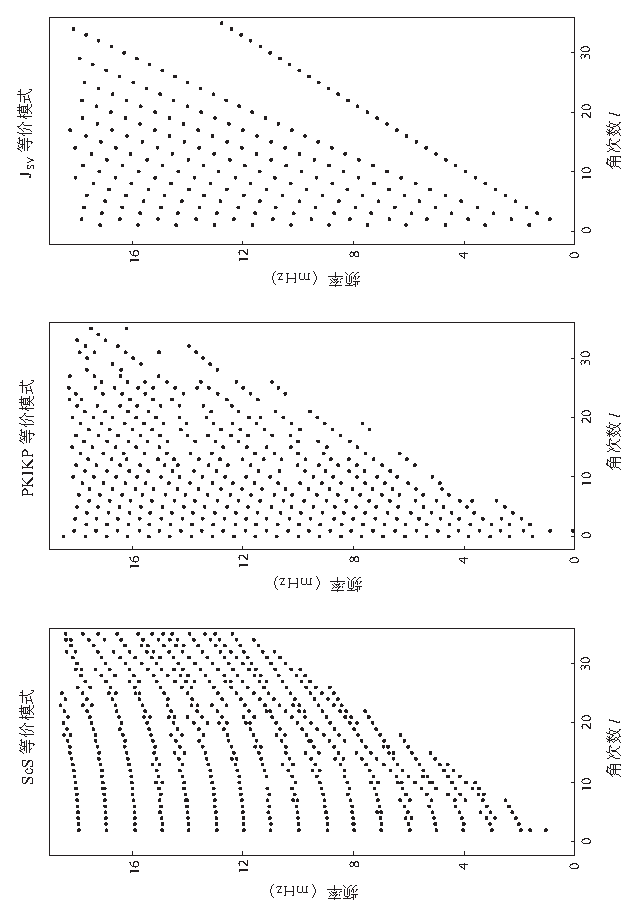
\includegraphics{../figures/chap08/fig12.eps}
}
\caption[threemodes]{
将阶数与频率较高的球型振荡划分为地幔~${\rm ScS}_{\rm SV}$~模式~({\em 左图\/})、PKIKP~模式~({\em 中图\/})~和内核~${\rm J}_{\rm SV}$~模式~({\em 右图\/})。${\rm ScS}_{\rm SV}$~模式有~$f_{\mu}>0.5$~和~$f_{\mu,\mbox{\scriptsize\,inner core}}\ll f_{\mu,\mbox{\scriptsize\,mantle}}$;PKIKP模式有~$f_{\kappa}>0.5$;${\rm J}_{\rm SV}$~模式有~$f_{\mu}>0.5$~和~$f_{\mu,\mbox{\scriptsize\,inner core}}\gg f_{\mu,\mbox{\scriptsize\,mantle}}$。
}
\label{fig:threemodes}
\end{sidewaysfigure}
第一类模式在接近纵轴时渐近群速度为~$d\om\hspace{-0.2 mm}/\hspace{-0.3 mm}dk\approx 0$,对应于地幔中相长干涉的~ScS${}_{\rm SV}$~体波;
\index{ScS-equivalent mode}%
\index{mode!ScS-equivalent}%
第二类具有中等群速度~$d\om\hspace{-0.2 mm}/\hspace{-0.3 mm}dk$,对应于整个地球内部的相长干涉的~PKIKP~波;
\index{PKIKP-equivalent mode}%
\index{mode!PKIKP-equivalent}%
最后的第三类具有最大的群速度~$d\om\hspace{-0.2 mm}/\hspace{-0.3 mm}dk$,对应于局限在固态内核中的相长干涉的~J${}_{\rm SV}$波;
\index{J-equivalent mode}%
\index{mode!J-equivalent}%
与ScS${}_{\rm SV}$~等价和与~J${}_{\rm SV}$~等价的模式分别是与~ScS${}_{\rm SH}$等价的地幔环型模式和与~J${}_{\rm SH}$~等价的内核环型模式~${}_n{\rm T}_l$~类似的球型振荡。对比图~\ref{fig:tormodefreqs}~和~\ref{fig:threemodes}~可知,ScS${}_{\rm SV}$~和~ScS${}_{\rm SH}$~的频散曲线近乎重叠;两者中~$l\approx 1$~的相邻本征频率之间的间隔约等于~$2\pi/\hspace{0.2 mm}T_{\rm ScS}$,其中~T${}_{\rm ScS}$~是垂直传播的剪切波往返走时。J${}_{\rm SV}$~和~J${}_{\rm SH}$~模式有相同的渐近群速度~$d\om\hspace{-0.2 mm}/\hspace{-0.3 mm}dk$~并在~$l\approx 1$~有相同的间距,即~$2\pi/\hspace{0.2 mm}T_{\rm J}$,其中~$T_{\rm J}$~是剪切波~J${}_{\rm SV}$~
或~J${}_{\rm SH}$~在内核传播所需要的时间;但与~ScS${}_{\rm SV}$~和~ScS${}_{\rm SH}$~模式不同,它们是相互交替的,如图~\ref{fig:incoremodes}~所示。
\begin{figure}
\begin{center}
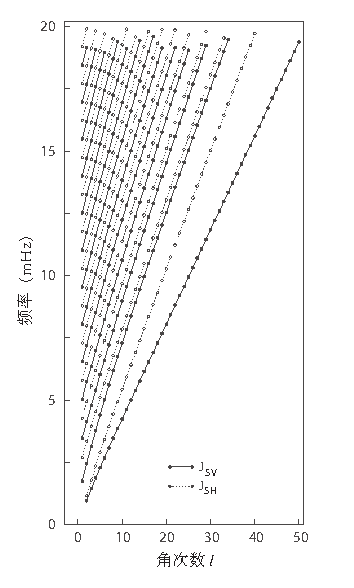
\includegraphics{../figures/chap08/fig13.eps}
\end{center}
\caption[innercoremodes]{\label{fig:incoremodes}
内核模式${\rm J}_{\rm SV}$~和~${\rm J}_{\rm SH}$~的本征频率。
\index{mode!inner-core}%
\index{inner-core mode}%
这两组频散曲线之间的相互交错可以归因于在接近地心折返时,${\rm J}_{\rm SV}$~波的水平分量符号发生反转,而~${\rm J}_{\rm SH}$~波则不变。
}
\end{figure}
每条~PKIKP~等价模式的频散曲线在角次数为零时以径向模式~${}_n{\rm S}_0$~终止。相邻径向模式本征频率之间的间距~${}_{n+1\hspace{-0.01in}}\om_0
-{}_n\om_0$~近似等于~$2\pi/\hspace{0.2 mm}T_{\rm PKIKP}$,其中~$T_{\rm PKIKP}$~是穿过地心的~PKIKP~波的走时。对阶数较高的高频球型模式划分为近似独立的~ScS${}_{\rm SV}$、J${}_{\rm SV}$~和~PKIKP~家族可以借助第~12~章中的模式-射线二象性的~JWKB~分析来理解。

从某种意义上说,图~\ref{fig:tormodefreqs}~中看似规则的环型模式频散图是一种假象:如果把地幔模式~${}_n{\rm T}_l$~和内核模式~${}_n{\rm C}_l$放在一起显示,并相应地重新赋予径向阶数~$n$,则“整个地球”的环型模式频散曲线将像球型模式频散曲线一样呈现出阶梯和紧密接触的特征。地幔和内核环型振荡由于中间存在的液态外核而完全解耦;因此,它们可以被独立考虑。相反,阶数较高的高频球型模式的三种类型之间只是近似独立的;行列式~(\ref{eq:8.det})~和~(\ref{eq:8.detfl})~不加区别地展现出所有三种类型的根;为此,它们{\em 必须\/}在同一个球型频散图中显示。

图~\ref{fig:ScS&J&PKIKP}~显示了几个二次球型模式~${}_n{\rm S}_2$~的径向和切向位移本征函数~$U$~和~$V$。
\begin{figure}
\begin{center}
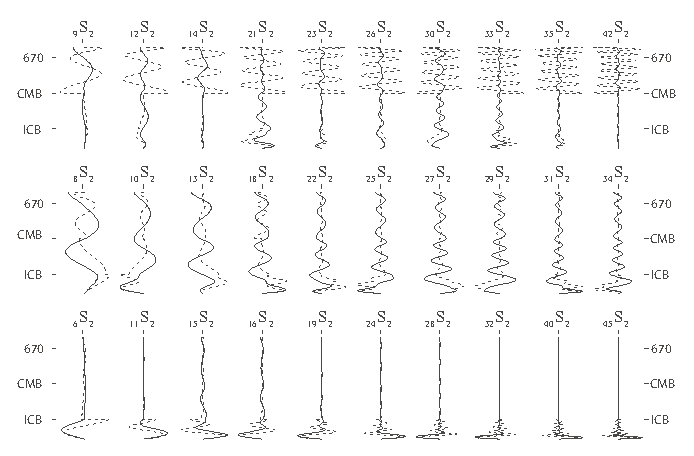
\includegraphics{../figures/chap08/fig14.eps}
\end{center}
\caption[ScS&J&PKIKP]{\label{fig:ScS&J&PKIKP}
\index{toroidal mode!inner-core}%
\index{mode!inner-core}%
\index{inner-core mode}%
按类型排列的几个~$l=2$~阶球型模式的本征函数~${}_nU_2$~({\em 实线\/})~和~${}_nV_2$~({\em 虚线\/}):${\rm ScS}_{\rm SV}$~模式~({\em 最上行\/}),PKIKP~模式~({\em 中间行\/})~和~${\rm J}_{\rm SV}$~模式~({\em 最下行\/})。径向阶数~$n$~和频率~${}_n\om_l$~向右逐渐增加。纵轴从自由表面延伸到地心;图中标明了~670~km~不连续面、核幔边界(CMB)和内核边界(ICB)的位置。
}
\end{figure}
ScS${}_{\rm SV}$~等价模式在地幔中有较大的、主要在切向的位移;
\index{ScS-equivalent mode}%
\index{mode!ScS-equivalent}%
PKIKP~等价模式在整个地球中有显著的、主要在径向的位移,
\index{PKIKP-equivalent mode}%
\index{mode!PKIKP-equivalent}%
J${}_{\rm SV}$~等价模式在固体内核外部的位移可以忽略不计;
\index{J-equivalent mode}%
\index{mode!J-equivalent}%
J${}_{\rm SV}$~模式仅在地心$r=0$附近才有显著径的向位移。
所有这些特征在图中右侧较高阶数的高频模式~${}_{42}{\rm S}_2$、${}_{34}{\rm S}_2$~和~${}_{45}{\rm S}_2$~中表现得最为明显。
一些低频模式是不太单纯的{\em 混合\/}模式;
\index{hybrid mode}%
\index{mode!hybrid}%
例如~${}_{21}{\rm S}_2$、${}_{30}{\rm S}_2$~和~${}_{33}{\rm S}_2$~这三个~${\rm ScS}_{\rm SV}$~模式以及~${}_{15}{\rm S}_2$~和~${}_{16}{\rm S}_2$~这两个~J${}_{\rm SV}$~模式均表现出次要的~PKIKP~特征(在整个地球中不可忽略的径向位移)。
解耦的~ScS${}_{\rm SH}$~和~J${}_{\rm SH}$~模式的环型位移本征函数~$W$~分别在地幔以外和内核以外完全为零;而高频~ScS${}_{\rm SV}$~和~J${}_{\rm SV}$~的本征函数虽然分别主要局限于地幔和内核,但处处都不为零。

图~\ref{fig:sphmodefreqs}~中,沿两条斜率约为~0.2 mHz/$l$~和~0.4 mHz/$l$~的明显的直线上的本征频率~$\omnl$~分别对应于附着在核幔边界和内核边界上的所谓的{\em 斯通利模式\/}。
\index{Stoneley mode}%
\index{mode!Stoneley}%
在固-液界面上的经典的斯通利波是无频散的(Stoneley \citeyear{stoneley24}; Scholte \citeyear{scholte47});这便是那些本征频率排列如此整齐原因。
\begin{figure}
\begin{center}
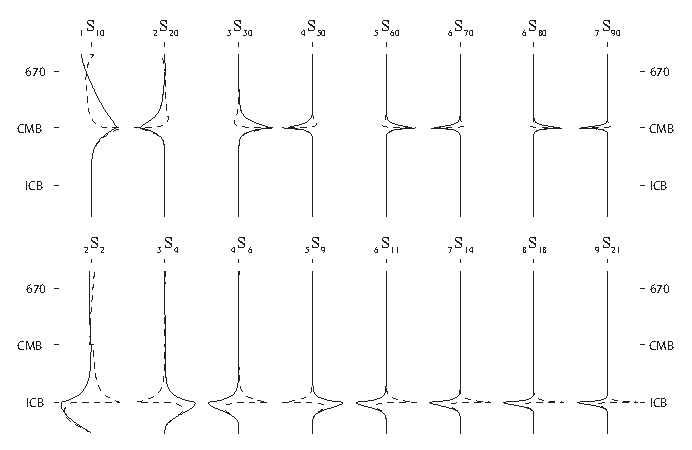
\includegraphics{../figures/chap08/fig15.eps}
\end{center}
\caption[Stoneley]{\label{fig:stoneley}
几个核幔边界(CMB)斯通利模式~({\em 上行\/})~与内核边界(ICB)斯通利模式~({\em 下行\/})~的本征函数~${}_nU_l$~({\em 实线\/})~和~${}_nV_l$~({\em 虚线\/})。纵轴从自由表面延伸到地心。
}
\end{figure}
图~\ref{fig:stoneley}~显示了几个核幔边界和内核边界斯通利模式的径向本函数~$\Unl$~和~$\Vnl$。径向位移表现出从边界处的最大值随着离开边界的距离以近似指数的形式减小,而切向位移在固态区域内有一个节点;随着频率的增加,位移越来越局限在边界附近。第一、第二和第三条J${}_{\rm SV}$等价模式的频散分支的本征函数与内核边界斯通利模式的本征函数有相似的特征,只是径向位移~$\Unl$~在内核中分别有一、二和三个节点。
实际上,内核斯通利模式构成了~J${}_{\rm SV}$~的“基阶”分支,而第一、第二和第三J${}_{\rm SV}$~分支则是~ICB~斯通利模式的“高阶模式”。内核振荡J${}_{\rm SV}$~和高频斯通利振荡都没有什么实际意义,因为他们不能被地壳或上地幔中的地震有效激发,也不能被位于地表的地震仪观测到。

\enlargethispage{-0.5mm}
图~\ref{fig:radeifs}~显示了前十个径向振荡的位移本征函数~${}_0U_0,\ldots,{}_9U_0$~和相应的牵引力~${}_0R_0,\ldots,{}_9R_0$;
\index{mode!radial}%
\index{radial mode}%
根据~Sturm~定理,径向位移节点数等于径向阶数~$n$。
\begin{figure}
\begin{center}
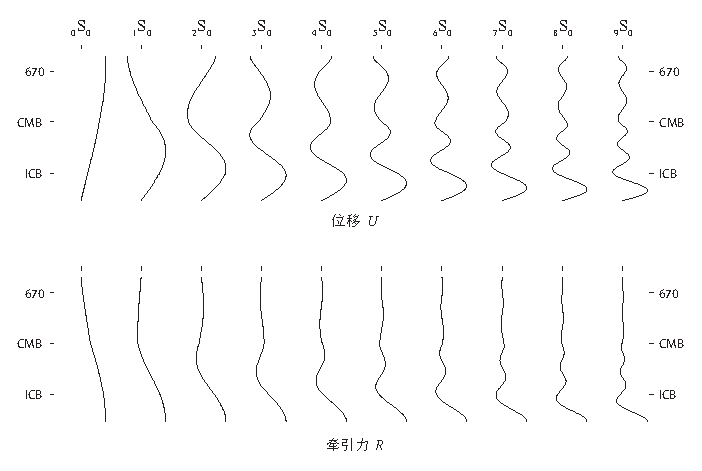
\includegraphics{../figures/chap08/fig16.eps}
\end{center}
\caption[radeifs]{\label{fig:radeifs}
前十个径向模式的位移~${}_nU_0$~({\em 上行\/})~和相应的牵引力~${}_nR_0$~({\em 下行\/})。纵轴从自由表面延伸到地心;图中标明了~670~km~不连续面、核幔边界(CMB)和内核边界(ICB)的位置。
}
\end{figure}
振荡的径向“波长”是等价的径向传播的~PKIKP~波的波长。地心附近的较大位移是因为渐近的~$r^{-1}$~的发散(见第~12.3.5~节)。如图~\ref{fig:0S0&0S2}~所展示的,在各向同性~PREM~模型中周期为~20.5~分钟的基阶径向模式~${}_0{\rm S}_0$~没有节点,且相当于一个大致均匀的压缩和膨胀,或整个地球向内和向外的“呼吸”。
\begin{figure}[!t]
\begin{center}
\scalebox{1.01}{
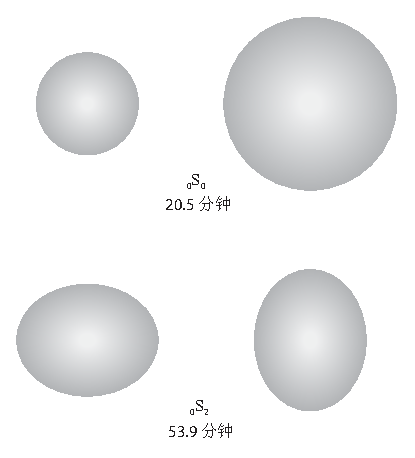
\includegraphics{../figures/chap08/fig17.eps}
}
\end{center}
\caption[0S2 mode]{\label{fig:0S0&0S2}
基阶径向模式~${}_0{\rm S}_0$~({\em 上行\/})~和橄榄球模式~${}_0{\rm S}_2$ 的~$m=0$~单态模式~({\em 下行\/})~示意图。图中所示为振荡周期的两个极端相位。
}
\end{figure}

观测到的最低频的地球自由振荡是著名的橄榄球模式~${}_0{\rm S}_2$,
\index{football mode}%
\index{mode!football}%
\index{fundamental mode!spheroidal}%
它在各向同性~PREM~模型中的周期为~53.9~分钟。其~$m=0$~的单态模式有一个形为~$\bs=\fourth(5/\pi)^{1/2}\,{}_0U_2(r)
(3\cos^2\theta-1)\hspace{0.3 mm}\brh
-\threehalves(5/6\pi)^{1/2}\,{}_0V_2(r)
\sin\theta\cos\theta\hspace{0.3 mm}\bthetah$的轴对称矢量位移场;地球表面交替地呈现瘦长和扁平的椭球形状,如图~\ref{fig:0S0&0S2}~所示。径向和切向本征函数~${}_0U_2$、${}_0V_2$~以及相应的牵引力~${}_0R_2$、${}_0S_2$~如图~\ref{fig:0S2}~所示。显然,运动涉及了整个地球。
\begin{figure}[!t]
\begin{center}
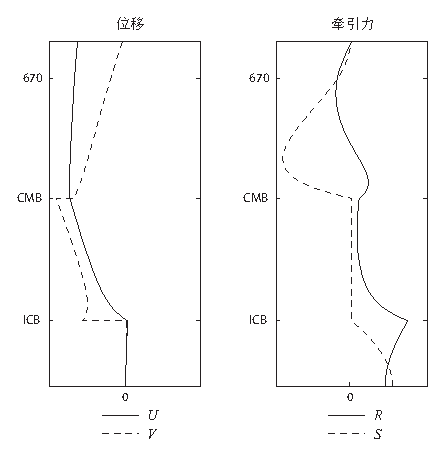
\includegraphics{../figures/chap08/fig18.eps}
\end{center}
\caption[0S2 mode]{\label{fig:0S2}
橄榄球模式~${}_0{\rm S}_2$~的位移本征函数~${}_0U_2$ 、${}_0V_2$~({\em 左图\/})~和相应的牵引力~${}_0R_2$、${}_0S_2$~({\em 右图\/})~的径向变化。纵轴从自由表面延伸到地心。图中标明了~670~km~不连续面、核幔边界(CMB)和内核边界(ICB)的位置。
}
\end{figure}
\enlargethispage{-0.5mm}

图~\ref{fig:sphmodefreqs}~中唯一更低频的振荡是~Slichter~模式或{\em 内核平动模式\/}~${}_1{\rm S}_1$,
\index{mode!Slichter}%
\index{Slichter mode}%
\index{translational inner-core mode}%
\index{mode!translational inner-core}%
其理论周期为~325~分钟或大约五个半小时!这个模式的存在是由~\textcite{slichter61}~首先提出的,它本质上是固态内核相对于液态外核和固态地幔的刚性平动;其位移~${}_1U_1$、${}_1V_1$~及相应的牵引力~${}_1R_1$、${}_1S_1$~如图~\ref{fig:1S1}~所示。
\begin{figure}[!t]
\begin{center}
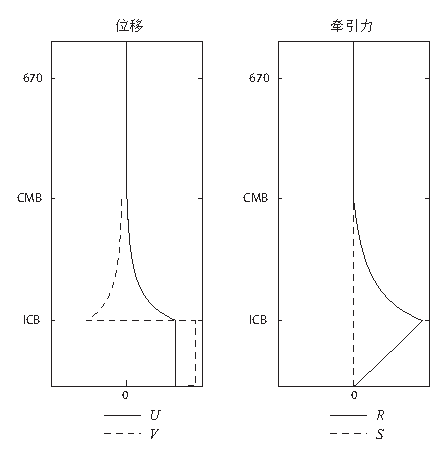
\includegraphics{../figures/chap08/fig19.eps}
\end{center}
\caption[1S1 mode]{\label{fig:1S1}
Slichter~或内核平动模式~${}_1{\rm S}_1$~的位移本征函数~${}_1U_1$ 、${}_1V_1$ ({\em 左图\/})~和相应的牵引力~${}_1R_1$、${}_1S_1$ ({\em 右图\/})~的径向变化。纵轴从自由表面延伸到地心。图中标明了~670~km~不连续面、核幔边界(CMB)和内核边界(ICB)的位置。
}
\end{figure}
在内核~$0\leq r\leq c$~中,径向和切向位移均为近似恒定~(${}_1V_1\approx\sqrt{2}\,{}_1U_1$);在外核~$c\leq r\leq b$~中,其运动表现为液体的“回流”,即液体必须让出位置以便内核能够移动。$m=-1$、$m=1$~以及~$m=0$~的单态模式分别对应于沿~$x$、$y$~和~$z$~轴的平动。Slichter~模式的本征频率~${}_1\om_1$~是一个强烈依赖于内核边界密度跃变函数,因为其主要恢复力是固态内核的负浮力(Smith \citeyear{smith76})。原则上,固态内核的平动可以被地球表面的重力仪观测到;然而,到目前为止,Slichter~模式并未被明确地检测到。内核和核幔边界的~Stoneley~模式以及~Slichter~模式对于~{\tt MINEOS}~和~{\tt OBANI}~等数值计算程序都是一个计算上的难题,因为需要施加边界条件~(\ref{eq:8.bfoa})的自由表面~$r=a$~本质上是一个节点。

\enlargethispage{-0.5\baselineskip}
表~8.2~列出了一些具有代表性的球型模式的压缩、剪切和重力势能占比。需要注意的是,在所有例子中,$f_{\kappa}+f_{\mu}+
f_{\rm g}=1$。重力势能占比最大的两种模式是~Slichter~模式~${}_1{\rm S}_1$~和橄榄球模式~${}_0{\rm S}_2$;这两个例子中,$\sV_{\rm g}$~都是正的,表明重力的作用是使变形的地球恢复到其平衡态的球对称构形,从物理的考虑上这是显而易见的。径向振荡~${}_n{\rm S}_0$~的负的重力势能反映了自重力对这些模式的失稳作用。还值得注意的是基阶径向模式~${}_0{\rm S}_0$~的极低的剪切能成分,它所包含的几乎是地球纯粹的压缩和膨胀。地幔的~ScS${}_{\rm SV}$~模式和内核的~J${}_{\rm SV}$~模式几乎将所有的能量以剪切形式储存,而~PKIKP~模式则将绝大部分的能量以压缩形式储存。PKIKP~模式的能量中有一部分(20$\%$~至~30$\%$)是剪切的,反映了地幔中的~P~波和固态内核中的~I~波的兼具压缩-剪切的混合性质。所有附着在边界上的模式,包括短周期瑞利波等价模式以及内核和核幔边界斯通利模式,都以剪切为主,只有很小一部分(10$\%$~到~20$\%$)的能量是压缩的。这是弹性界面波的一个特征。

\begin{table}
\centering
\index{fractional energy}%
\index{energy!fractional}%
\begin{tabular}{|r|r|c|c|r|l|} \hline
& & & & & \\
模式 & mHz \hspace{1.3 mm} & $f_{\kappa}$ & $f_{\mu}$
& $f_{\rm g}$\hspace{3.0 mm} & 名称或描述\\
& & & & & \\ \hline
& & & & & \\
${}_0{\rm S}_0$\hspace{1.7 mm} & 0.8143 & 1.30 & 0.03 & $-0.33$ & 基阶径向 \\
${}_1{\rm S}_0$\hspace{1.7 mm} & 1.6313 & 0.95 & 0.16 & $-0.11$ & 径向高阶 \\
${}_2{\rm S}_0$\hspace{1.7 mm} & 2.5105 & 0.88 & 0.17 & $-0.05$ & 径向高阶 \\
& & & & & \\
${}_0{\rm S}_2$\hspace{1.7 mm} & 0.3093 & 0.12 & 0.55 & 0.33 & 橄榄球模式 \\
${}_0{\rm S}_3$\hspace{1.7 mm} & 0.4686 & 0.16 & 0.65 & 0.19 & 梨子模式 \\
& & & & & \\
${}_0{\rm S}_{10}$\hspace{0.4 mm} & 1.7265 & 0.23 & 0.81 & $-0.04$ & 基阶瑞利 \\
${}_0{\rm S}_{20}$\hspace{0.4 mm} & 2.8784 & 0.20 & 0.81 & $-0.01$ & 基阶瑞利 \\
${}_0{\rm S}_{30}$\hspace{0.4 mm} & 3.8155 & 0.16 & 0.85 & $-0.01$ & 基阶瑞利 \\
${}_0{\rm S}_{40}$\hspace{0.4 mm} & 4.7101 & 0.14 & 0.86 & $-0.00$ & 基阶瑞利 \\
& & & & & \\
${}_{10}{\rm S}_6$\hspace{1.7 mm} & 4.9142 & 0.03 & 1.01 & $-0.04$ & 内核~J${}_{\rm SV}$ \\
${}_{16}{\rm S}_3$\hspace{1.7 mm} & 6.2225 & 0.02 & 1.02 & $-0.04$ & 内核~J${}_{\rm SV}$ \\
${}_{24}{\rm S}_8$\hspace{1.7 mm} & 10.8312 & 0.04 & 0.99 & $-0.03$ & 内核~J${}_{\rm SV}$ \\
& & & & & \\
${}_{14}{\rm S}_3$\hspace{1.7 mm} & 5.4075 & 0.03 & 0.98 & $-0.02$ & 地幔~ScS${}_{\rm SV}$ \\
${}_{17}{\rm S}_6$\hspace{1.7 mm} & 7.5806 & 0.10 & 0.92 & $-0.02$ & 地幔~ScS${}_{\rm SV}$ \\
${}_{24}{\rm S}_5$\hspace{1.7 mm} & 9.6478 & 0.02 & 0.99 & $-0.02$ & 地幔~ScS${}_{\rm SV}$ \\
& & & & & \\
${}_{11}{\rm S}_5$\hspace{1.7 mm} & 5.0744 & 0.72 & 0.30 & $-0.02$ & PKIKP \\
${}_{16}{\rm S}_6$\hspace{1.7 mm} & 7.1537 & 0.75 & 0.26 & $-0.01$ & PKIKP \\
${}_{27}{\rm S}_2$\hspace{1.7 mm} & 9.8653 & 0.80 & 0.21 & $-0.01$ & PKIKP \\
& & & & & \\
${}_1{\rm S}_{10}$\hspace{0.4 mm} & 2.1484 & 0.14 & 0.80 & 0.06 & 核幔边界斯通利 \\
${}_2{\rm S}_{18}$\hspace{0.4 mm} & 3.8745 & 0.20 & 0.77 & 0.03 & 核幔边界斯通利 \\
& & & & & \\
${}_3{\rm S}_4$\hspace{1.7 mm} & 1.8333 & 0.08 & 0.93 & $-0.01$ & 内外核边界斯通利 \\
${}_6{\rm S}_{11}$\hspace{0.4 mm} & 4.5350 & 0.06 & 0.94 & $-0.00$ & 内外核边界斯通利 \\
& & & & & \\
${}_1{\rm S}_1$\hspace{1.5 mm} & 0.0513 & 0.64 & 0.00 & 0.36 & Slichter 模式 \\
& & & & & \\ \hline
\end{tabular}
\caption[modeenergy]{
一些球型模式的频率~$\omega/2\pi$(mHz)和压缩、剪切以及重力势能占比。表中所列数值是基于各项同性~PREM~地球模型;缩写CMB和ICB分别代表核幔边界和内核边界。
}
\label{table:modenergy}
\end{table}

\enlargethispage{-0.5\baselineskip}
在赋予辨识符号~${}_n{\rm S}_l$~时,便利的做法是包含所有的以弹性为主的模式,包括内核~J${}_{\rm SV}$~模式和斯通利模式。由此而来的命名规则的一个令人烦恼之处是它依赖于地球模型。为说明这一点,我们考虑一个~PKIKP~等价模式~${}_n{\rm S}_l$~和一个~J${}_{\rm SV}$~等价模式~${}_{n+1\hspace{-0.01in}}{\rm S}_l$,在某一给定的地球模型中它们的本征频率非常接近一个交叉规避点,因而几乎相等。假设现在将固态内核中的剪切波速$\beta$略微减小,但保持压缩波速~$\alpha$~处处不变;J${}_{\rm SV}$~模式的频率~${}_{n+1\hspace{-0.01in}}\om_l$~将略微下降,而~PKIKP~模式的频率~${}_n\om_l$~则基本不变。如果~$\beta$~的变化足够大,这一改变将导致两个模式互换身份,从而使~${}_n{\rm S}_l$~变成内核模式~J${}_{\rm SV}$,而${}_{n+1\hspace{-0.01in}}{\rm S}_l$~变成~PKIKP~模式。例如,观测到的~SNREI~频率为~4.04~mHz~的~PKIKP~模式,在平均内核剪切波速为~$\beta\approx3.6$~km/s的地球模型~1066A~中为~${}_{10}{\rm S}_2$,而在平均内核剪切波速为~$\beta\approx3.5$~km/s的地球模型~1066B~中为~${}_{11}{\rm S}_2$(Gilbert \& Dziewonski \citeyear{gilbert&dziewonski75})。这种近似简并的~PKIKP~和~J${}_{\rm SV}$~模式的其它例子还有~${}_6{\rm S}_2$--\hspace{0.2 mm}${}_7{\rm S}_2$、${}_5{\rm S}_{10}$--\hspace{0.2 mm}${}_6{\rm S}_{10}$~和~${}_{11}{\rm S}_8$--\hspace{0.2 mm}${}_{12}{\rm S}_8$。

\renewcommand{\thesubsection}{$\!\!\!\raise1.3ex\hbox{$\star$}\!\!$
\arabic{chapter}.\arabic{section}.\arabic{subsection}}
%\subsection{Tsunami and core gravity modes}
\subsection{海啸与地核重力模式}
\index{mode!tsunami|(}%
\index{mode!core gravity|(}%
\index{tsunami|(}%
\index{core gravity mode|(}%
\index{gravity mode|(}%
\index{exotic mode|(}%
\index{mode!exotic|(}%
\renewcommand{\thesubsection}{\arabic{chapter}.\arabic{section}.\arabic{subsection}}

\begin{figure}[!b]
\begin{center}
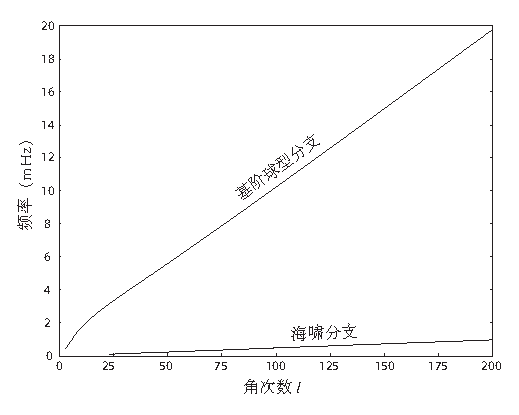
\includegraphics{../figures/chap08/fig20.eps}
\end{center}
\caption[tsunami branch]{
\label{fig:8.20}
经修改的具有~4~公里厚度海水层的~PREM~模型的频散图中海啸模式和基阶球型模式的比较。在~$l\leq 200$~时,海啸模式可以很好的近似为是无频散的。
}
\end{figure}
除了上面讨论的以弹性为主的模式,像~PREM~一样接近真实的~SNREI~地球模型还有两种以重力为主的球型振荡,它们都没有被显示在图~\ref{fig:sphmodefreqs}~中,也没有在赋予辨识符号~${}_n{\rm S}_l$时加以考虑。这些“奇特的”球型振荡中第一种是海水的表面重力或{\em 海啸模式\/}。图~\ref{fig:8.20}~将海啸模式的本征频率与~${}_0{\rm S}_l$~分支上的模式做了比较;显然,将~${}_0{\rm S}_l$~命名为地球的“基阶”球型模式分支是不恰当的!
\index{fundamental mode!spheroidal}%
如图~\ref{fig:8.21}~所展示的,海啸模式的位移本征函数主要局限于均匀的海水中。
\begin{figure}[!b]
\begin{center}
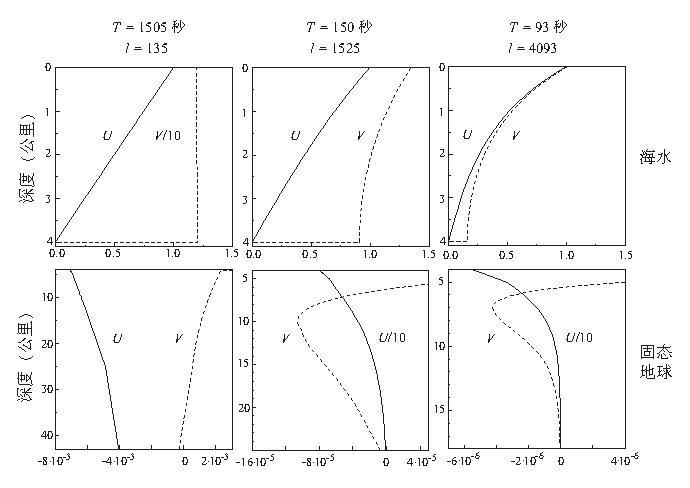
\includegraphics{../figures/chap08/fig21.eps}
\end{center}
\caption[tsunami displacements]{
\label{fig:8.21}
海啸模式的位移本征函数~$U$~({\em 实线\/})和~$V$~({\em 虚线\/})。从左至右,周期分别为~1505、150~和~93~秒,对应的角次数分别为~$l=135$、$l=1525$~和~$l=4093$。({\em 上行\/})~4 km~海水层内的本征函数。({\em 下行\/})固体地球中本征函数的放大视图。在所有例子中,纵轴表示海面以下深度~$z=a-r$;请注意在固体中不同的深度比例。为便于显示,所有不同周期的本征函数都做了在~$z=0$~处~$U=1$~的归一化。
}
\end{figure}
在~1505~秒的周期(角次数~$l=135$~),海水中径向本征函数~$U$~大约比切向本征函数~$V$~小十倍,也就是说海水来回晃动但几乎没有自由表面的变形。此外,$V$~在海水中几乎是恒定的,而~$U$~从表面的最大值以大致线性减小到海床几乎为零。这些都是无频散浅水表面重力波的特征~(Lamb \citeyear{lamb32}; Lighthill \citeyear{lighthill78})。对于海水下面的固体地球,相应的位移~$U$~和~$V$~比海水中的位移小两个数量级以上;一个~1505~秒的海啸只能“感觉”到固体地球中~50~km~左右的深度。在周期~150~秒~($l\approx 1500$)~时,海水中的径向和切向位移大小相当;相应的固体地球位移要小几乎四个数量级,且仅能“感觉”到海床以下约~20~km~的深度。最后,在周期~93~秒($l\approx 4000$)时,$U$~和~$V$~在海水中几乎相等;两者均呈现随深度~$z$~的近似指数衰减~$\exp(-kz/a)$,这是深水表面重力波的特征。伴随这种~90~秒的海啸的固体地球位移在海床以下~10~公里深度完全可以忽略不计。浅水和深水特征之间的转换发生在~50到100~秒之间;周期更短的海啸模式无法被地震激发,因为它们根本不知道下面有固体地球的存在。因此,海啸的主要观测周期是几百到几千秒。即使在长周期,整个固体地球实际上显然是一个变形的节点;这当然也是为什么只有大型的海底浅源地震才能引发海啸。所有海啸模式的势能~$\sV_{\kappa}+\sV_{\mu}+\sV_{\rm g}$~有~95$\%$~以上为重力势能。Ward~(\citeyear{ward80})~率先将~SNREI-地球简正模式理论用于研究海啸的产生和传播;Okal~(\citeyear{okal82})~对海啸模式分支的频散做了渐近分析。

液态地核重力模式,也叫做地核{\em 低阶模式\/},是第二种“奇特的”重力振荡。
\index{undertone}%
这些尚未观测到的模式的理论本征频率对于液态外核中~Brunt-V\"{a}is\"{a}l\"{a}~频率~$N$~的径向分布十分敏感。如果在整个外核~$c\leq r\leq b$中处处有~$N^2>0$,那么会存在无穷多个低阶模式,它们有实数的本征频率,范围为~$0\leq\om\leq N_{\rm max}$;另一方面,如果在~$c\leq r\leq b$~中处处有~$N^2<0$,则存在无穷多个本征频率为纯虚数~($\om^2<0$)~的不稳定低阶模式。用地震本征频率观测值所约束的模型一般在地核中具有~$N^2>0$~与~$N^2<0$~交替变化的区域;这样会有~$\om^2>0$~和~$\om^2<0$~两种地核模式,相应的本征函数分别主要局限于稳定和不稳定的层内。对于任何特定的最佳拟合模型(如~PREM~),这些低阶振荡的细节都没有什么意义,因为对地核中的~$N$~约束很差。如果液态地核是中性分层的(同时没有地表的海水层),因而~$\earth_{\rm F}$~中处处有~$N=0$,则不存在非平凡的重力模式。这种中性分层模型反而具有无限维的地转本征空间,相应的简并本征频率为~$\om=0$,如第~8.8.2~节所述。

将~(\ref{eq:8.Vfl})--(\ref{eq:8.Kfl})这几个方程适当地合并,可以得到如下关系
\eq
\label{8.funny}
\om^2\frac{d}{dr}(rV)=\om^2\sqL U-\sqL N^2(\rho g)^{-1}R,
\en
$\earth_{\rm F}$~中所有模式都必须满足上式。在液态外核的任何中性分层区域,方程~(\ref{8.funny})~对平凡模式都成立,因为~$\om=0$。对于~$\om\not=0$的非平凡模式,方程~(\ref{8.funny})~在$N=0$时简化为~$\dV+r^{-1}V-\sqL r^{-1}U=0$。在一个具有中性分层液态外核的地球模型中,所有非平凡球型振荡都必须满足这一简单关系,包括以弹性为主的振荡~${}_n{\rm S}_l$。
\index{mode!tsunami|)}%
\index{mode!core gravity|)}%
\index{tsunami|)}%
\index{core gravity mode|)}%
\index{gravity mode|)}%
\index{exotic mode|)}%
\index{mode!exotic|)}%

\renewcommand{\thesubsection}{$\!\!\!\raise1.3ex\hbox{$\star$}\!\!$
\arabic{chapter}.\arabic{section}.\arabic{subsection}}
%\subsection{Atmospheric modes}
\subsection{大气模式}
\index{mode!atmospheric|(}%
\index{atmospheric mode|(}%
\renewcommand{\thesubsection}{\arabic{chapter}.\arabic{section}.\arabic{subsection}}

从原则上来讲,地球大气层的存在可以通过将~(\ref{eq:8.Vfl})--(\ref{eq:8.Kfl})~这四个流体动力学方程从海水层表面继续向上积分来处理,并在海水-大气界面~$r=a$~施加连续性条件~$[U]^+_-=0$、$[P]^+_-=0$、$[R]^+_-=0$和$[B]^+_-=0$。在~$r\rightarrow\infty$~极限(实际上是高程~$r-a\approx 200$~km~)~下,有必要施加一个依赖频率的边界条件,来规定向外辐射到密度$\rho$和不可压缩性$\kappa$均为无穷小的外大气层中的声波-重力能~(Watada \citeyear{watada95};Lognonn\'{e}, Cl\'{e}v\'{e}d\'{e} \& Kanamori
\citeyear{lognonne&al98})。具有上覆大气层的地球模型除了已经讨论过的模式之外,还有一组丰富的受大气的~Brunt-V\"{a}is\"{a}l\"{a}~频率~$N$~控制的以重力为主的模式和受大气的声速~$\alpha =(\kappa/\hspace{-0.2 mm}\rho)^{1/2}$~控制的以声波为主的模式。后者可以很好地近似看成是无频散的,其本征频率~$\omega$~在~$0\leq l\leq 100$~范围内基本上与角次数无关,如图~\ref{8.fig.atmodes}~所示。
\begin{figure}[!t]
\begin{center}
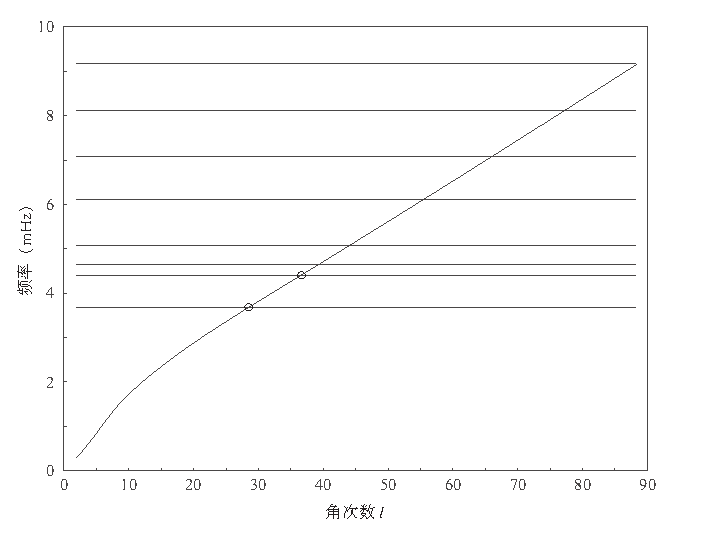
\includegraphics{../figures/chap08/fig22.eps}
\end{center}
\caption[atmospheric modes]{\label{8.fig.atmodes}
基阶和前七个高阶声波模的实数本征频率~$\omega/2\pi$的频散图。小到可以忽略的群速度~$d\omega/dk\approx 0$~表明与之相关的大气声波的传播几乎是无频散的。相交的曲线是基阶地幔球型模式~${}_0{\rm S}_l$~的频散曲线。小圆圈标记在角次数~$l=28\!-\!29$ ($\omega/2\pi= 3.68$~mHz)~和~$l=36\!-\!37$ ($\omega/2\pi= 4.40$~mHz)~处的两个交点。
}
\end{figure}
表~8.3~总结了基阶和前七个高阶声波模式的频率和品质因子。其衰减几乎完全是由于能量的向外辐射;这些模式有一个很小的指数尾巴延伸到下面的固-液地球;然而,地幔内部的固有衰减效应并不显著。只有基阶和第一个高阶模式有~$Q>10$;高阶模式较低的品质因子表明它们不是完全被限制在大气中的。

基阶地震模式分支~${}_0{\rm S}_l$~分别在~$l=28\!-\!29$和$l=36\!-\!37$处与前两个大气模式分支相交。相近的本征频率增强了固-液地球与大气之间的耦合;受此影响的模式~${}_0{\rm S}_{28}\!-\!{}_0{\rm S}_{29}$和${}_0{\rm S}_{36}\!-\!{}_0{\rm S}_{37}$~其大气能量含量可以高达~0.04$\%$。正因如此,频率为~$\om/2\pi\approx 3.68$~mHz~(周期~$T\approx 272$~s)~和~$\om/2\pi\approx 4.40$~mHz~(周期~$T\approx 227$~s)~的基阶球型振荡可以被强烈的大气源所激发。1982~年墨西哥~El Chich\'{o}n~和~1991~年菲律宾~Pinatubo~火山喷发之后首次探测到这种近似单频的振荡~(Kanamori \& Mori \citeyear{kanamori&mori92}; Widmer \& Zirn \citeyear{widmer&zurn92b}; Zirn \& Widmer \citeyear{zurn&widmer96})。角次数为~$l\approx 28\!-\!29$~和~$l\approx36\!-\!37$~的大气模式同样可以被固体地球内部的源所激发。这也为在大地震之后偶有报道的微气压和电离层扰动现象提供了解释~(Mikumo \citeyear{mikumo68}; Yuen, Weaver, Suzuki \& Furumoto \citeyear{yuen&al69})。
\begin{table}[!t]
\centering
\begin{tabular}{|c|c|c|c|c|c|c|c|c|} \hline
& & & & & & & & \\
\hspace{-0.1 mm}频率 (mHz)\hspace{-0.1 mm}
& \hspace{-0.1 mm}3.68\hspace{-0.1 mm} &
\hspace{-0.1 mm}4.40\hspace{-0.1 mm} &
\hspace{-0.1 mm}4.65\hspace{-0.1 mm} &
\hspace{-0.1 mm}5.07\hspace{-0.1 mm} &
\hspace{-0.1 mm}6.10\hspace{-0.1 mm} &
\hspace{-0.1 mm}7.07\hspace{-0.1 mm} &
\hspace{-0.1 mm}8.11\hspace{-0.1 mm} &
\hspace{-0.1 mm}9.16\hspace{-0.1 mm} \\
& & & & & & & & \\ \hline
& & & & & & & & \\
品质因子 & 117 & 21 & 3 & 9 & 6 & 7 & 7 & 8 \\
& & & & & & & & \\ \hline
\end{tabular}
\caption[atm modes]{
在无频散范围~$0\leq l\leq 100$~内的以声波为主的大气模式的理论频率~$\omega/2\pi$~和品质因子~$Q$~(Lognonn\'{e}, Cl\'{e}v\'{e}d\'{e} \& Kanamori
\citeyear{lognonne&al98})。在$a=6371$~km~以外的密度~$\rho$~和声速~$\alpha$~来自美国标准大气~(U.S. Standard Atmosphere)模型;内部的固-液地球模型为~PREM。
}
\label{table:atmmodes}
\end{table}

在本书的剩余部分,为简单起见,我们将继续假设固-液地球~$\earth$~的自由表面~$\p\earth$~之外的区域~$\allspace -\earth$~为真空。
\index{mode!atmospheric|)}%
\index{atmospheric mode|)}%
\index{mode!spheroidal|)}%
\index{spheroidal mode|)}%

\renewcommand{\thesection}{$\!\!\!\raise1.3ex\hbox{$\star$}\!\!$
\arabic{chapter}.\arabic{section}}
%\section{Transversely Isotropic Earth Model}
\section{横向各向同性地球模型}
\index{Earth model!SNREI|(}%
\index{SNREI Earth model|(}%
\index{Earth model!transversely isotropic|(}%
\label{sec:8.transverse}
\renewcommand{\thesection}{\arabic{chapter}.\arabic{section}}

根据定义,一个球对称地球模型是在所有围绕其中心的刚性旋转下不变的模型。具有这一特性的最普遍的四阶弹性张量~$\bGamma$~不是各向同性的,而是有径向对称轴的{\em 横向各向同性\/}张量(Love \citeyear{love27}; Stoneley \citeyear{stoneley49}):
\index{transverse isotropy}%
\index{elastic tensor!transversely isotropic}%
\index{tensor!elastic!transversely isotropic}%
\eqa
\lefteqn{\bGamma=C\,\brh\brh\brh\brh+A(\bthetah\bthetah\bthetah\bthetah
+\bphih\bphih\bphih\bphih)} \nonumber \\
&&\mbox{}+F(\brh\brh\bthetah\bthetah
+\bthetah\bthetah\brh\brh+\brh\brh\bphih\bphih+\bphih\bphih\brh\brh)
\nonumber \\
&&\mbox{}\quad+(A-2N)(\bthetah\bthetah\bphih\bphih
+\bphih\bphih\bthetah\bthetah)
\nonumber \\
&&\mbox{}\quad\quad+N(\bthetah\bphih\bthetah\bphih
+\bphih\bthetah\bphih\bthetah+\bthetah\bphih\bphih\bthetah
+\bphih\bthetah\bthetah\bphih) \nonumber \\
&&\mbox{}\quad\quad\quad+L(\brh\bthetah\brh\bthetah+\bthetah\brh\bthetah\brh
+\brh\bthetah\bthetah\brh+\bthetah\brh\brh\bthetah \nonumber \\
&&\mbox{}\quad\quad\quad\quad+\brh\bphih\brh\bphih+\bphih\brh\bphih\brh
+\brh\bphih\bphih\brh+\bphih\brh\brh\bphih).
\label{eq:8.bGamma}
\ena
一个一般的球对称、横向各向同性地球模型可通过给定其密度~$\rho$~以及五个弹性参数~$C$、$A$、$L$、$N$~和~$F$~的径向变化来表述。在这样的地球模型中,地幔和固态内核中局部的弹性体波波速是不随方位变化的,但它们依赖于偏振以及波矢量和局部径向轴之间的倾角。我们也可以不用~$C$、$A$、$L$、$N$~和~$F$这些参数,而是给定垂直和水平传播的压缩波波速~$\alpha_{\rm v}=(C\hspace{-0.3 mm}/\hspace{-0.3 mm}\rho)^{1/2}$和$\alpha_{\rm h}=(A/\hspace{-0.3 mm}\rho)^{1/2}$、垂直和水平传播的~SH-偏振的剪切波波速~$\beta_{\rm v}=(L/\hspace{-0.3 mm}\rho)^{1/2}$和$\beta_{\rm h}=(N\hspace{-0.3 mm}/\hspace{-0.3 mm}\rho)^{1/2}$,以及无量纲参数~$\eta=F/(A-2L)$。在横向各向同性地球模型中垂直传播的剪切波不会有任何分裂;所有偏振均以速度~$\beta_{\rm v}$~传播。垂直和水平传播的~SV-偏振波均有相同的速度,因而~$\beta_{\rm v}$~可被解释为垂直传播的~SH~波波速或水平传播的~SV~波波速。横向各向同性地球模型的不可压缩性和刚度的定义为
\index{incompressibility}%
\index{rigidity}%
\index{modulus!bulk}%
\index{bulk modulus}%
\index{shear modulus}%
\index{modulus!shear}%
\eq \label{8.kappadef}
\kappa=\ninth(C+4A-4N+4F),
\en
\eq
\label{8.mudef}
\mu=\fifteenth(C+A+6L+5N-2F).
\en
这些是“等价的”各向同性模型的参数,
\index{equivalent isotropic parameter}%
其弹性张量~$\bGamma'$~在~(\ref{3.kappamudef2})~所表示的最小二乘意义上是~$\bGamma$~的最佳近似;(\ref{8.kappadef})--(\ref{8.mudef})~两式是~(\ref{3.kappamudef1})~的特例。在各向异性为零的极限情况下,有$C=A=\kappa+\fourthirds\mu$,$L=N=\mu$~和~$F=\kappa-\twothirds\mu$;因而有~$\alpha_{\rm v}=\alpha_{\rm h}=\alpha$,$\beta_{\rm v}=\beta_{\rm h}=\beta$~和$\eta=1$。地球的液态区域必须是各项同性的,有~$C=A=F=\kappa$~和~$L=N=0$。最后我们指出,一个最普遍的球对称地球模型也可能具有横向各向同性的初始应力张量,其形式为~$-p_{\rm v}\hspace{0.2 mm}\brh\brh-p_{\rm h}(\bthetah\bthetah
+\bphih\bphih)$;我们将忽略这种可能性,而假设~$p_{\rm v}=p_{\rm h}=p$。图~\ref{fig:anisoprem}~显示了横向各向同性版本的PREM~模型中~$\alpha_{\rm v}$、$\alpha_{\rm h}$、$\beta_{\rm v}$、$\beta_{\rm h}$~和~$\eta$~的径向变化(Dziewonski \& Anderson \citeyear{dziewonski&anderson81})。
\index{Preliminary Reference Earth Model (PREM)}%
模型中只有在~24.4 km到220~km~深度之间的最上部地幔是各向异性的;在该区域中,垂直传播的~P~波和~S~波比水平传播的要慢~$2\%$~到~$4\%$。

频率域的动量方程~(\ref{eq:8.smeq})~和动力学边界条件~(\ref{eq:8.df})--(\ref{eq:8.dfs})~适用于任何球对称地球模型;唯一的差别是本构关系~(\ref{eq:8.constitutive})~必须用~$\bT=\bGamma\!:\!\beps$~替换,其中~$\bGamma$~由~(\ref{eq:8.bGamma})~式给定。
\index{constitutive relation!transversely isotropic}%
只要~(\ref{eq:8.splagrangian}) 和~(\ref{eq:8.splagrang2})中的弹性能量密度~$\kappa(\bdel\cdot\bs)^2+2\mu(\bd\!:\!\bd)$~用~$\beps\!:\!\bGamma\!:\!\beps$~来取代,位移和位移-势函数形式的瑞利原理中也均适用于横向各向同性地球模型。我们仍然可以使用第~\ref{sec:8.radscaleqns}~节中介绍的三种方法之中的任何一种,来将控制的矢量和张量方程转换为等价的径向标量方程组。无论怎样进行转换,我们会看到结果自然地分解为解耦的球型和环型本征值问题,如同在~SNREI~地球中一样。我们将在第~8.9.1~节和第~8.9.2~节中分别考虑这两种振荡,还是同前文一样,首先从较简单的环型模式开始。
\begin{figure}[!t]
\begin{center}
\scalebox{0.95}{
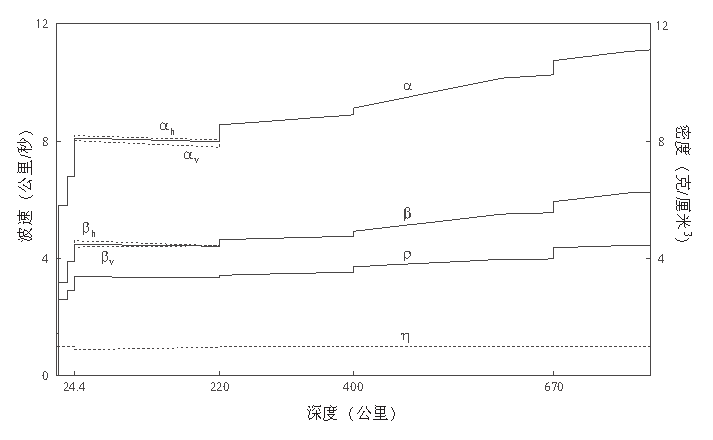
\includegraphics{../figures/chap08/fig23.eps}
}
\end{center}
\caption[anisotropicPREM]{\label{fig:anisoprem}
虚线显示初步参考地球模型~(PREM)~中在上地幔垂直和水平传播的压缩波和剪切波波速~$\alpha_{\rm v}$、$\alpha_{\rm h}$、$\beta_{\rm v}$ 、$\beta_{\rm h}$~和各向异性参数~$\eta$。实线显示密度~$\rho$以及“等价的”各向同性模型的压缩波和剪切波波速~$\alpha$~和~$\beta$,以便比较。所有波速都是频率为~$\omega/2\pi=1$~Hz~的波所“感觉”到的。
\index{shear-wave speed!PREM}%
\index{S-wave speed!PREM}%
\index{compressional-wave speed!PREM}%
\index{P-wave speed!PREM}%
\index{speed!shear-wave}%
\index{speed!compressional-wave}%
\index{density!PREM}%
}
\end{figure}

\renewcommand{\thesubsection}{$\!\!\!\raise1.3ex\hbox{$\star$}\!\!$
\arabic{chapter}.\arabic{section}.\arabic{subsection}}
%\subsection{Toroidal oscillations}
\subsection{环型振荡}
\index{toroidal mode|(}%
\index{mode!toroidal|(}%
\renewcommand{\thesubsection}{\arabic{chapter}.\arabic{section}.\arabic{subsection}}

横向各向同性地球模型的环型振荡有形如~$\bs=W\bC_{lm}$的位移矢量和相应的形如~$\brh\cdot\bT=T\bC_{lm}$的牵引力矢量,其中
\eq
T=L(\dW-r^{-1}W).
\en
这些模式满足的的径向作用量积分~$\sI_{\rm T}$~为~(\ref{8.spheractor})式,其中
\index{Lagrangian density!toroidal modes}%
\eq
L_{\rm T}=\half[\om^{2\!}\rho W^2
-L(\dW-r^{-1}W)^2-(\sqL^2-2)Nr^{-2}W^2].
\label{eq:8.torti}
\en
这里的环型拉格朗日量密度~$L_{\rm T}$,以及我们将在下面引入的球型拉格朗日量密度~$L_{\rm S}$、$L_{\rm S}^{\prime}$~和~$L_{\rm R}$~都不要与用同一符号表示的弹性参数~$L$~混淆。根据上下文,其含义应该始终是清楚的,即使在密度中忽略了下角标~T、S~和~R时,如我们在第~9.4~节中要做的那样。欧拉-拉格朗日方程~(\ref{8.EULERW})~等价于一阶常微分方程组:
\eq
\dW=r^{-1}W+L^{-1}T, \label{eq:8.Wtifo}
\en
\eq
\dT=[-\om^{2\!}\rho+(\sqL^2-2)Nr^{-2}]W-3r^{-1}T.
\label{eq:8.Ttifo}
\en
这些方程必须在当~$r=d_{\rm FS}$~和~$r=a$~时~$T=0$~这一边界条件下求解。环型模式的弹性势能完全以剪切形式储存;
\index{energy!toroidal mode}%
\index{elastic energy}%
总的动能加势能为~$\sE=\half(\om^2\sT+\sV_{\rm e})$,其中
\eq
\sV_{\rm e}=\int_0^a[L(\dW-r^{-1}W)^2+(\sqL^2-2)Nr^{-2}W^2]\,r^2dr.
\en
值得注意的是,环型简正模式仅依赖于密度~$\rho$~和两个弹性参数~$L$~和~$N$,或者等价地只依赖于密度~$\rho$~和两个~SH~波波速~$\beta_{\rm v}$~和~$\beta_{\rm h}$。由于有弹性约束~$L\geq 0$~以及~$N\geq 0$,横向各向同性地球的环型模式总是稳定的,即~$\om^2=\sV_{\rm e}/\sT\geq 0$。
\index{toroidal mode|)}%
\index{mode!toroidal|)}%

\renewcommand{\thesubsection}{$\!\!\!\raise1.3ex\hbox{$\star$}\!\!$
\arabic{chapter}.\arabic{section}.\arabic{subsection}}
%\subsection{Spheroidal oscillations}
\subsection{球型振荡}
\index{spheroidal mode|(}%
\index{mode!spheroidal|(}%
\renewcommand{\thesubsection}{\arabic{chapter}.\arabic{section}.\arabic{subsection}}

球型振荡的位移矢量和牵引力矢量的形式分别为~$\bs=U\bP_{lm}+V\bB_{lm}$~和~$\brh\cdot\bT=R\bP_{lm}+S\bB_{lm}$,其中
\eq
R=C\dU+Fr^{-1}(2U-\sqL V), \label{eq:8.Rti}
\en
\eq
S=L(\dV-r^{-1}V+\sqL r^{-1}U). \label{eq:8.Sti}
\en
位移和位移-势函数形式的径向作用量积分~$\sI_{\rm S}$~和~$\sI_{\rm S}^{\prime}$~分别为~(\ref{8.spheract})式和(\ref{8.Iprime})式,其中
\index{Lagrangian density!spheroidal modes}%
\eqa
\lefteqn{L_{\rm S}=\half[\om^{2\!}\rho(U^2+V^2)
-C\dU^{\raisebox{-0.4ex}{$\scriptstyle 2$}}
-2Fr^{-1}\dU(2U-\sqL V)} \label{eq:8.spherti}
\nonumber \\
&&\mbox{}-(A-N)r^{-2}(2U-\sqL V)^2
-L(\dV-r^{-1}V+\sqL r^{-1}U)^2 \nonumber \\
&&\mbox{}\qquad-(\sqL^2-2)Nr^{-2}V^2-\rho(U\dP+\sqL r^{-1}VP)
\nonumber \\
&&\mbox{}\qquad\qquad-4\pi G\rho^2U^2
+2\rho gr^{-1}U(2U-\sqL V)],
\ena
\eqa
\lefteqn{L_{\rm S}^{\prime}=\half[\om^{2\!}\rho(U^2+V^2)
-C\dU^{\raisebox{-0.4ex}{$\scriptstyle 2$}}
-2Fr^{-1}\dU(2U-\sqL V)} \label{eq:8.sphertip}
\nonumber \\
&&\mbox{}-(A-N)r^{-2}(2U-\sqL V)^2
-L(\dV-r^{-1}V+\sqL r^{-1}U)^2 \nonumber \\
&&\mbox{}\qquad-(\sqL^2-2)Nr^{-2}V^2-2\rho(U\dP+\sqL r^{-1}VP)
\nonumber \\
&&\mbox{}\qquad\qquad-4\pi G\rho^2U^2
+2\rho gr^{-1}U(2U-\sqL V) \nonumber \\
&&\mbox{}\qquad\qquad\qquad-(4\pi G)^{-1}
(\dP^{\raisebox{-0.7ex}{$\scriptstyle 2$}}+\sqL^2r^2P^2)].
\ena
欧拉-拉格朗日方程~(\ref{8.Euler1})--(\ref{8.EULERV})~和~(\ref{8.dPLprime})~等价于以下六元一阶方程组:
\eq \label{eq:8.tiU}
\dU=-2C^{-1}Fr^{-1}U
+\sqL C^{-1}Fr^{-1}V
+C^{-1}R,
\en
\eq
\dV=-\sqL r^{-1}U+r^{-1}V+L^{-1}S, \label{eq:8.tiV}
\en
\eq
\dP=-4\pi G\rho U-(l+1)r^{-1\!}P+B, \label{eq:8.tiP}
\en
\eqa \label{eq:8.tiR}
\lefteqn{\dR=[-\om^{2\!}\rho-4\rho gr^{-1}
+4(A-N-C^{-1}F^2)r^{-2}]U} \nonumber \\
&&\mbox{}+[\sqL\rho gr^{-1}-2\sqL(A-N-C^{-1}F^2)r^{-2}]V \nonumber \\
&&\mbox{}\qquad-2(1-C^{-1}F)r^{-1}R
+\sqL r^{-1}S \nonumber \\
&&\mbox{}\qquad\qquad-(l+1)\rho r^{-1}P+\rho B,
\ena
\eqa \label{eq:8.tiS}
\lefteqn{\dS=[\sqL\rho g r^{-1}
-2\sqL(A-N-C^{-1}F^2)r^{-2}]U} \nonumber \\
&&\mbox{}-[\om^{2\!}\rho+2Nr^{-2}
-\sqL^2(A-C^{-1}F^2)r^{-2}]V \nonumber \\
&&\mbox{}\qquad-\sqL C^{-1}Fr^{-1}R 
-3r^{-1}S
+\sqL\rho r^{-1}P,
\ena
\eq
\dot{B}=-4\pi G(l+1)\rho r^{-1}U+4\pi G\sqL\rho r^{-1}V+(l-1)r^{-1}B.
\label{eq:8.tiK}
\en
这些方程必须在当~$r=a$~时~$R=0$和$B=0$~以及当~$r=a$~和~$r=d_{\rm FS}$~时~$S=0$~的边界条件下求解。球型振荡总的动能加势能为~$\sE=\half(\om^2\sT+\sV_{\rm e}+\sV_{\rm g})$,其中
\index{energy!spheroidal mode}%
\index{elastic energy}%
\eqa
\lefteqn{\sV_{\rm e}=\int_0^a
[C\dU^{\raisebox{-0.4ex}{$\scriptstyle 2$}}
+2Fr^{-1}\dU(2U-\sqL V)+(A-N)r^{-2}(2U-\sqL V)^2}
\nonumber \\
&&\mbox{}+L(\dV-r^{-1}V+\sqL r^{-1}U)^2
+(\sqL^2-2)Nr^{-2}V^2]\,r^2dr,
\ena
$\sV_{\rm g}$~与前面一样仍由~(\ref{eq:8.Vgrav})~给定。球型模式依赖于密度~$\rho$~和全部五个弹性参数~$C$、$A$、$L$、$N$~和~$F$。Backus (\citeyear{backus67})最早推导出六元控制方程组~(\ref{eq:8.tiU})--(\ref{eq:8.tiK})。

\renewcommand{\thesubsection}{$\!\!\!\raise1.3ex\hbox{$\star$}\!\!$
\arabic{chapter}.\arabic{section}.\arabic{subsection}}
%\subsection{Radial oscillations}
\subsection{径向振荡}
\index{radial mode|(}%
\index{mode!radial|(}%
\renewcommand{\thesubsection}{\arabic{chapter}.\arabic{section}.\arabic{subsection}}

横向各向同性地球模型的径向模式满足的径向作用量~$\sI_{\rm R}$~的形式为~(\ref{8.RADACT}),其中
\index{Lagrangian density!radial modes}%
\eq \label{8.RADTI}
L_{\rm R}=\half[\om^{2\!}\rho\hspace{0.2 mm}U^2
-C\dU^{\raisebox{-0.6ex}{$\scriptstyle 2$}}
-4Fr^{-1}\dU U-4(A-N)r^{-2}U^2].
\en
\begin{figure}[!b]
\begin{center}
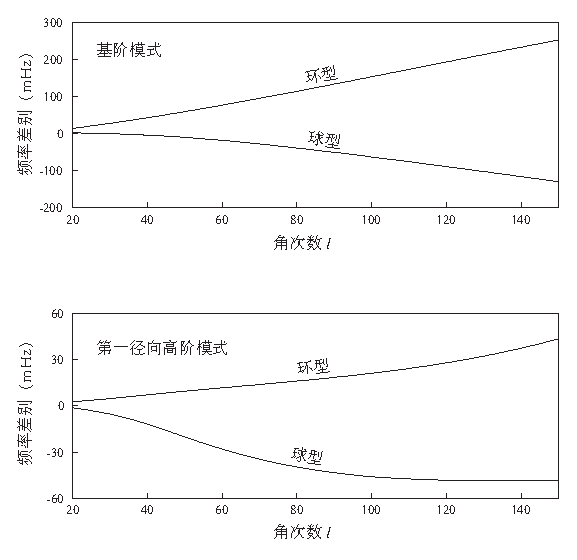
\includegraphics{../figures/chap08/fig24.eps}
\end{center}
\caption[TIversusIfreqs]{\label{fig:TIversusI}
横向各向同性~(TI)~和“等价”的各向同性~(EI)~PREM~模型的基阶模式({\em 上图\/})和第一个高阶模式({\em 下图\/})的本征频率的差别~$\omega_{\rm TI}-\omega_{\rm EI}$。
}
\end{figure}
欧拉-拉格朗日方程~(\ref{8.RADEL})~等价于以下二元一阶方程组
\eq \label{8.tirad1}
\dU=-2C^{-1}Fr^{-1}U+C^{-1}R,
\en
\eqa \label{8.tirad2}
\lefteqn{
\dR=[-\om^{2\!}\rho+4(A-N-C^{-1}F^2)-4\rho gr^{-1}]U} \nonumber \\
&&\mbox{}\qquad\qquad-2(1-C^{-1}F)r^{-1}R,
\ena
这些方程必须在当~$r=a$~时~$R=0$~的边界条件下求解。径向模式的能量为~$\sE=\half(\om^2\sT+\sV_{\rm e}+\sV_{\rm g})$,其中
\index{elastic energy}%
\index{energy!radial mode}%
\eq
\sV_{\rm e}=\int_0^a[C\dU^{\raisebox{-0.6ex}{$\scriptstyle 2$}}
+4Fr^{-1}\dU U+4(A-N)r^{-2}U^2]\,r^2dr,
\en
$\sV_{\rm g}$~由~(\ref{8.radgrav})~式给定。径向振荡依赖于密度~$\rho$~和~$C$、$A$ 、$N$~和~$F$这四个参数,与第五个弹性参数~$L$~无关。
\index{radial mode|)}%
\index{mode!radial|)}%
\index{spheroidal mode|)}%
\index{mode!spheroidal|)}%

\renewcommand{\thesubsection}{$\!\!\!\raise1.3ex\hbox{$\star$}\!\!$
\arabic{chapter}.\arabic{section}.\arabic{subsection}}
%\subsection{Effect upon the eigenfrequencies}
\subsection{对本征频率的影响}
\renewcommand{\thesubsection}{\arabic{chapter}.\arabic{section}.\arabic{subsection}}

综上所述,通过对~SNREI~地球模型所得到的公式做非常有限的改变,就可以计算横向各向同性地球模型的弹性-重力本征频率和本征函数。这些改变均已纳入~{\tt MINEOS\/}~和~{\tt OBANI\/}~这两个程序,使它们能够处理各向同性或横向各向同性地球模型。图~\ref{fig:TIversusI}~展示了~PREM~模型的横向各向同性对基阶和第一个高阶频散分支上的~${}_0{\rm S}_l$、${}_0{\rm T}_l$~和~${}_1{\rm S}_l$ ,${}_1{\rm T}_l$~的本征频率的影响。显示的量是横向各向同性模型与“等价”的各向同性模型的本征频率之间的差别~$\om_{\rm TI}-\om_{\rm EI}$。对~$\beta_{\rm h}$的依赖性比~$\beta_{\rm v}$更强的基阶环型本征频率~${}_0\om^{\rm T}_l$有~0.5\hspace{0.2 mm}--\hspace{0.2 mm}1.5$\%$的升高,而基本上与~$\beta_{\rm h}$~无关的基阶球型本征频率~${}_0\om^{\rm S}_l$却因各向异性而降低了~0.3\hspace{0.2 mm}--\hspace{0.2 mm}1$\%$。第一个高阶分支上的本征频率~${}_1\om^{\rm T}_l$~和~${}_1\om^{\rm S}_l$也有类似的但弱得多的影响。PREM~模型中横向各向同性的引入最初是为了
协调观测到的角次数~$l$~大于~40\hspace{0.2 mm}--\hspace{0.2 mm}50~的基阶瑞利波等价模式~${}_0{\rm S}_l$~和勒夫波等价模式~${}_0{\rm T}_l$~的本征频率。近来的分析已经减小了这种差异的幅度(Widmer \citeyear{widmer91}; Ekstr\"{o}m, Tromp \& Larson \citeyear{ekstrom&al96}),目前尚不清楚究竟是否需要或是多强的上地幔各向异性来拟合全球平均的基阶模式数据。
